\documentclass[12pt,]{article}
\usepackage{lmodern}
\usepackage{amssymb,amsmath}
\usepackage{ifxetex,ifluatex}
\usepackage{fixltx2e} % provides \textsubscript
\ifnum 0\ifxetex 1\fi\ifluatex 1\fi=0 % if pdftex
  \usepackage[T1]{fontenc}
  \usepackage[utf8]{inputenc}
\else % if luatex or xelatex
  \ifxetex
    \usepackage{mathspec}
    \usepackage{xltxtra,xunicode}
  \else
    \usepackage{fontspec}
  \fi
  \defaultfontfeatures{Mapping=tex-text,Scale=MatchLowercase}
  \newcommand{\euro}{€}
    \setmainfont{Palatino}
    \setsansfont{Century Gothic}
    \setmonofont[Mapping=tex-ansi]{Consolas}
\fi
% use upquote if available, for straight quotes in verbatim environments
\IfFileExists{upquote.sty}{\usepackage{upquote}}{}
% use microtype if available
\IfFileExists{microtype.sty}{%
\usepackage{microtype}
\UseMicrotypeSet[protrusion]{basicmath} % disable protrusion for tt fonts
}{}
\ifxetex
  \usepackage[setpagesize=false, % page size defined by xetex
              unicode=false, % unicode breaks when used with xetex
              xetex]{hyperref}
\else
  \usepackage[unicode=true]{hyperref}
\fi
\hypersetup{breaklinks=true,
            bookmarks=true,
            pdfauthor={Amin Meyghani},
            pdftitle={Introduction to Angular 2},
            colorlinks=true,
            citecolor=blue,
            urlcolor=blue,
            linkcolor=magenta,
            pdfborder={0 0 0}}
\urlstyle{same}  % don't use monospace font for urls
\usepackage{fancyhdr}
\pagestyle{fancy}
\pagenumbering{arabic}
\lhead{\itshape Introduction to Angular 2}
\chead{}
\rhead{\itshape{\nouppercase{\leftmark}}}
\lfoot{}
\cfoot{}
\rfoot{\thepage}
\usepackage{color}
\usepackage{fancyvrb}
\newcommand{\VerbBar}{|}
\newcommand{\VERB}{\Verb[commandchars=\\\{\}]}
\DefineVerbatimEnvironment{Highlighting}{Verbatim}{commandchars=\\\{\}}
% Add ',fontsize=\small' for more characters per line
\newenvironment{Shaded}{}{}
\newcommand{\KeywordTok}[1]{\textcolor[rgb]{0.00,0.00,1.00}{{#1}}}
\newcommand{\DataTypeTok}[1]{{#1}}
\newcommand{\DecValTok}[1]{{#1}}
\newcommand{\BaseNTok}[1]{{#1}}
\newcommand{\FloatTok}[1]{{#1}}
\newcommand{\ConstantTok}[1]{{#1}}
\newcommand{\CharTok}[1]{\textcolor[rgb]{0.00,0.50,0.50}{{#1}}}
\newcommand{\SpecialCharTok}[1]{\textcolor[rgb]{0.00,0.50,0.50}{{#1}}}
\newcommand{\StringTok}[1]{\textcolor[rgb]{0.00,0.50,0.50}{{#1}}}
\newcommand{\VerbatimStringTok}[1]{\textcolor[rgb]{0.00,0.50,0.50}{{#1}}}
\newcommand{\SpecialStringTok}[1]{\textcolor[rgb]{0.00,0.50,0.50}{{#1}}}
\newcommand{\ImportTok}[1]{{#1}}
\newcommand{\CommentTok}[1]{\textcolor[rgb]{0.00,0.50,0.00}{{#1}}}
\newcommand{\DocumentationTok}[1]{\textcolor[rgb]{0.00,0.50,0.00}{{#1}}}
\newcommand{\AnnotationTok}[1]{\textcolor[rgb]{0.00,0.50,0.00}{{#1}}}
\newcommand{\CommentVarTok}[1]{\textcolor[rgb]{0.00,0.50,0.00}{{#1}}}
\newcommand{\OtherTok}[1]{\textcolor[rgb]{1.00,0.25,0.00}{{#1}}}
\newcommand{\FunctionTok}[1]{{#1}}
\newcommand{\VariableTok}[1]{{#1}}
\newcommand{\ControlFlowTok}[1]{\textcolor[rgb]{0.00,0.00,1.00}{{#1}}}
\newcommand{\OperatorTok}[1]{{#1}}
\newcommand{\BuiltInTok}[1]{{#1}}
\newcommand{\ExtensionTok}[1]{{#1}}
\newcommand{\PreprocessorTok}[1]{\textcolor[rgb]{1.00,0.25,0.00}{{#1}}}
\newcommand{\AttributeTok}[1]{{#1}}
\newcommand{\RegionMarkerTok}[1]{{#1}}
\newcommand{\InformationTok}[1]{\textcolor[rgb]{0.00,0.50,0.00}{{#1}}}
\newcommand{\WarningTok}[1]{\textcolor[rgb]{0.00,0.50,0.00}{\textbf{{#1}}}}
\newcommand{\AlertTok}[1]{\textcolor[rgb]{1.00,0.00,0.00}{{#1}}}
\newcommand{\ErrorTok}[1]{\textcolor[rgb]{1.00,0.00,0.00}{\textbf{{#1}}}}
\newcommand{\NormalTok}[1]{{#1}}
\usepackage{longtable,booktabs}
\usepackage{graphicx,grffile}
\makeatletter
\def\maxwidth{\ifdim\Gin@nat@width>\linewidth\linewidth\else\Gin@nat@width\fi}
\def\maxheight{\ifdim\Gin@nat@height>\textheight\textheight\else\Gin@nat@height\fi}
\makeatother
% Scale images if necessary, so that they will not overflow the page
% margins by default, and it is still possible to overwrite the defaults
% using explicit options in \includegraphics[width, height, ...]{}
\setkeys{Gin}{width=\maxwidth,height=\maxheight,keepaspectratio}
\setlength{\parindent}{0pt}
\setlength{\parskip}{6pt plus 2pt minus 1pt}
\setlength{\emergencystretch}{3em}  % prevent overfull lines
\providecommand{\tightlist}{%
  \setlength{\itemsep}{0pt}\setlength{\parskip}{0pt}}
\setcounter{secnumdepth}{5}

\title{Introduction to Angular 2}
\author{Amin Meyghani}
\date{}

% Redefines (sub)paragraphs to behave more like sections
\ifx\paragraph\undefined\else
\let\oldparagraph\paragraph
\renewcommand{\paragraph}[1]{\oldparagraph{#1}\mbox{}}
\fi
\ifx\subparagraph\undefined\else
\let\oldsubparagraph\subparagraph
\renewcommand{\subparagraph}[1]{\oldsubparagraph{#1}\mbox{}}
\fi

\begin{document}
\maketitle

{
\hypersetup{linkcolor=black}
\setcounter{tocdepth}{5}
\tableofcontents
}
\section{Notes}\label{notes}

\begin{itemize}
\item
  The book assumes that you are working in a Unix-like environment. If
  you are on Windows you can use \href{https://www.cygwin.com/}{Cygwin}
  so that you can follow along with the bash terminal commands.
\item
  All the project files for the book are hosted on github:
  \url{https://github.com/aminmeyghani/angular2-intro}. You can clone
  the repository and check out the project files. Throughout the book,
  you will see references to the project files. Those refer to this
  repository. For example,
  \texttt{angular2-intro/project-files/hello-angular} refers to the
  \texttt{hello-angular} folder inside the \texttt{project-files}
  folder.
\item
  Make sure you have \texttt{git} installed on your machine. That is,
  make sure you get an output for \texttt{git\ -\/-version}.
\item
  The book assumes that you have a working knowledge of JavaScript and
  Angular 1.x
\item
  Node is heavily used throughout the book. Make sure that you follow
  the ``Node'' chapter to install Node and set permissions correctly.
\item
  All the keyboard shortcuts are mac-based. But if you are using a
  non-mac machine, you can almost always replace \texttt{command} with
  \texttt{ctrl} and you should be good. For example, if you a see a
  shortcut like \texttt{command\ +\ shift\ +\ b}, you can use
  \texttt{ctrl\ +\ shift\ +\ b} where \texttt{ctrl} is obviously the
  \texttt{control} key!
\end{itemize}

\section{Installing Node}\label{installing-node}

You can use \href{https://github.com/creationix/nvm}{nvm} to install and
manage Node on your machine. Copy the install script and run it:

\begin{verbatim}
curl -o- https://raw.githubusercontent.com/creationix/nvm/v0.30.1/install.sh | bash
\end{verbatim}

After that, make a new terminal window and make sure that it is
installed, by running:

\begin{verbatim}
nvm --help
\end{verbatim}

Now you can use \texttt{nvm} to install Node \texttt{0.12.9} by running:

\begin{verbatim}
nvm install 0.12.9
\end{verbatim}

After that, nvm is going to load version 0.12.9 automatically. If it
doesn't, you can load it in the current shell, with:

\begin{verbatim}
nvm use 0.12.9
\end{verbatim}

Note that you can load any node version in the current shell with
\texttt{nvm\ use\ 0.x.y} after installing that version.

Also note that if you want to make \texttt{0.12.9} the default Node
version on your machine, you can do so by running the following:

\begin{verbatim}
nvm alias default 0.12.9
\end{verbatim}

Then you can verify that it is the default version by making a new
terminal window and typing \texttt{node\ -v}.

\subsection{Permissions}\label{permissions}

Never use \texttt{sudo} to install packages, never do
\texttt{sudo\ npm\ install\ \textless{}package\textgreater{}}. If you
get permission errors while installing without \texttt{sudo}, you can
own the folders instead. So for example, if you get an error like:

\begin{verbatim}
Error: EACCES, mkdir '/usr/local'
\end{verbatim}

you can own the folder with:

\begin{verbatim}
sudo chown -R `whoami` /usr/local
\end{verbatim}

You can own folders until Node doesn't complain.

\subsection{\texorpdfstring{Installing
\texttt{live-server}}{Installing live-server}}\label{installing-live-server}

Install a package to verify that node is installed and everything is
wired up correctly. We are going to use \texttt{live-server} through the
book. So let's install that with:

\begin{verbatim}
npm i -g live-server
\end{verbatim}

Then, you should be able to run \texttt{live-server} in any folder to
serve the content of that folder:

\begin{verbatim}
mdkir ~/Desktop/sample && cd $_
live-server .
\end{verbatim}

\section{Visual Studio Code}\label{visual-studio-code}

Visual Studio Code is a good IDE for developing web apps. In this
chapter we will look at installing and configuring VSCode.

\subsection{Visual Studio Code Basics}\label{visual-studio-code-basics}

\begin{itemize}
\item
  Install Visual Studio Code from: \url{https://code.visualstudio.com/}
\item
  You can open new projects by going to the
  \texttt{File\ \textgreater{}\ Open} tag, to etierh open a folder
  containing your project or a single file
\item
  Some useful keyboard shortcuts are:

  \begin{itemize}
  \tightlist
  \item
    \texttt{command\ +\ b}: to close/open the file navigator
  \item
    \texttt{command\ +\ shift\ +\ p}: to open the prompt
  \end{itemize}
\item
  To install extensions open the prompt with
  \texttt{command\ +\ shift\ +\ p} and type:

\begin{verbatim}
> install extension
\end{verbatim}
\item
  You can change the keyboard shortcuts settings from
  \texttt{Preferences\ \textgreater{}\ Keyboard\ Shortcuts}. Open the
  settings and then you can add your own shortcuts:

\begin{verbatim}
// Place your key bindings in this file to overwrite the defaults
[
  {
    "key": "cmd+t",
    "command": "workbench.action.quickOpen"
  },
  {
    "key": "shift+cmd+r",
    "command": "editor.action.format",
    "when": "editorTextFocus"
  }
]
\end{verbatim}
\end{itemize}

\subsection{Setting up VSCode for
TypeScript}\label{setting-up-vscode-for-typescript}

In this section we are going to set up Visual Studio Code for
TypeScript. The project files for this chapter are in
\href{https://github.com/aminmeyghani/angular2-intro/tree/master/project-files/vscode}{\textbf{\texttt{angular2-intro/project-files/vscode}}}.
You can either follow along or check out the folder to see the final
result.

\subsubsection{Installing TypeScript}\label{installing-typescript}

Before anything, we need to install the TypeScript compiler. You can
install the TypeScript compiler with npm:

\begin{verbatim}
npm i typescript -g
\end{verbatim}

Then to verify that it is installed, run \texttt{tsc\ -v} to see the
version of the compiler. You will get an output like this:

\begin{verbatim}
message TS6029: Version 1.7.5
\end{verbatim}

In addition to the compiler, we also need to install the TypeScript
Definition manager for DefinitelyTyped (tsd). You can install tsd with:

\begin{verbatim}
npm i tsd -g
\end{verbatim}

Using TSD, you can search and install TypeScript definition files
directly from the community driven DefinitelyTyped repository. To verify
that tsd is installed, run tsd with the \texttt{version} flag:

\begin{verbatim}
tsd --version
\end{verbatim}

You should get an output like this:

\begin{verbatim}
>> tsd 0.6.5
\end{verbatim}

After \texttt{tsd} and \texttt{tsc} are installed, we can compile a
hello world program:

make a file called \texttt{hello.ts} on your desktop:

\begin{verbatim}
touch ~/Desktop/hello.ts
\end{verbatim}

Then, put some TypeScript code in the file:

\begin{verbatim}
echo "const adder = (a: number, b: number): number => a + b;" > ~/Desktop/hello.ts
\end{verbatim}

Then you can compile the file to JavaScript:

\begin{verbatim}
tsc ~/Desktop/hello.ts
\end{verbatim}

It should output a file in \texttt{Desktop/hello.js}:

\begin{Shaded}
\begin{Highlighting}[numbers=left,,]
\KeywordTok{var} \NormalTok{adder }\OperatorTok{=} \KeywordTok{function} \NormalTok{(a}\OperatorTok{,} \NormalTok{b) }\OperatorTok{\{} \ControlFlowTok{return} \NormalTok{a }\OperatorTok{+} \NormalTok{b}\OperatorTok{;} \OperatorTok{\};}
\end{Highlighting}
\end{Shaded}

Now that your TypeScript compiler setup, we can move on to configuring
Visual Studio Code.

\subsubsection{Add VSCode
Configurations}\label{add-vscode-configurations}

\begin{itemize}
\item
  First download and install Visual Studio Code from the VSCode
  \href{https://code.visualstudio.com/}{Website}
\item
  After installing VSCode, open it and then make a new window:
  \texttt{File\ \textgreater{}\ New\ Window}
\item
  Then, make a folder on your desktop for a new project:
  \texttt{mkdir\ \textasciitilde{}/Desktop/vscode-demo}
\item
  After that, open the folder in VSCode:
  \texttt{File\ \textgreater{}\ open} and select the
  \texttt{vscode-demo} folder on your desktop.
\item
  Now we need to make three configuration files:

  \begin{enumerate}
  \def\labelenumi{\arabic{enumi}.}
  \tightlist
  \item
    \href{http://json.schemastore.org/tsconfig}{\texttt{tsconfig.json}}:
    configuration for the TypeScript compiler
  \item
    \texttt{tasks.json}: Task configuration for VSCode to watch and
    compile files
  \item
    \texttt{launch.json}: Configuration for the debugger
  \end{enumerate}
\end{itemize}

The \texttt{tsconfig.json} file should be in the root of the project.
Let's make the file and put the following in it:

\begin{Shaded}
\begin{Highlighting}[numbers=left,,]
\OperatorTok{\{}
  \StringTok{"compilerOptions"}\OperatorTok{:} \OperatorTok{\{}
    \StringTok{"experimentalDecorators"}\OperatorTok{:} \KeywordTok{true}\OperatorTok{,}
    \StringTok{"emitDecoratorMetadata"}\OperatorTok{:} \KeywordTok{true}\OperatorTok{,}
    \StringTok{"module"}\OperatorTok{:} \StringTok{"commonjs"}\OperatorTok{,}
    \StringTok{"target"}\OperatorTok{:} \StringTok{"es5"}\OperatorTok{,}
    \StringTok{"sourceMap"}\OperatorTok{:} \KeywordTok{true}\OperatorTok{,}
    \StringTok{"outDir"}\OperatorTok{:} \StringTok{"output"}\OperatorTok{,}
    \StringTok{"watch"}\OperatorTok{:} \KeywordTok{true}
  \OperatorTok{\}}
\OperatorTok{\}}
\end{Highlighting}
\end{Shaded}

Now to make the \texttt{tasks.json} file. Open the prompt with
\texttt{command\ +\ shift\ +\ p} and type:

\begin{verbatim}
> configure task runner
\end{verbatim}

Then put the following in the file and save the file:

\begin{Shaded}
\begin{Highlighting}[numbers=left,,]
\OperatorTok{\{}
  \StringTok{"version"}\OperatorTok{:} \StringTok{"0.1.0"}\OperatorTok{,}
  \StringTok{"command"}\OperatorTok{:} \StringTok{"tsc"}\OperatorTok{,}
  \StringTok{"showOutput"}\OperatorTok{:} \StringTok{"silent"}\OperatorTok{,}
  \StringTok{"isShellCommand"}\OperatorTok{:} \KeywordTok{true}\OperatorTok{,}
  \StringTok{"problemMatcher"}\OperatorTok{:} \StringTok{"$tsc"}
\OperatorTok{\}}
\end{Highlighting}
\end{Shaded}

The last thing that we need to set up is the debugger, i.e.~the
\texttt{launch.json} file. Right click on the \texttt{.vscode} folder in
the file navigator and make a new file called \texttt{launch.json} and
put in the following:

\begin{Shaded}
\begin{Highlighting}[numbers=left,,]
\OperatorTok{\{}
  \StringTok{"version"}\OperatorTok{:} \StringTok{"0.1.0"}\OperatorTok{,}
  \StringTok{"configurations"}\OperatorTok{:} \NormalTok{[}
    \OperatorTok{\{}
      \StringTok{"name"}\OperatorTok{:} \StringTok{"TS Debugger"}\OperatorTok{,}
      \StringTok{"type"}\OperatorTok{:} \StringTok{"node"}\OperatorTok{,}
      \StringTok{"program"}\OperatorTok{:} \StringTok{"main.ts"}\OperatorTok{,}
      \StringTok{"stopOnEntry"}\OperatorTok{:} \KeywordTok{false}\OperatorTok{,}
      \StringTok{"sourceMaps"}\OperatorTok{:} \KeywordTok{true}\OperatorTok{,}
      \StringTok{"outDir"}\OperatorTok{:} \StringTok{"output"}
    \OperatorTok{\}}
  \NormalTok{]}
\OperatorTok{\}}
\end{Highlighting}
\end{Shaded}

After you save the file, you should be able to see the debugger in the
debugger dropdown options.

Now, we are ready to make the \texttt{main.ts} file in the root of the
project:

\textbf{\texttt{main.ts}}

\begin{Shaded}
\begin{Highlighting}[numbers=left,,]
\DataTypeTok{const} \NormalTok{sum = (a: number, b: number): number => a + b;}
\DataTypeTok{const} \NormalTok{r = }\FunctionTok{sum}\NormalTok{(}\DecValTok{1}\NormalTok{,}\DecValTok{2}\NormalTok{);}
\NormalTok{console.}\FunctionTok{log}\NormalTok{(r);}
\end{Highlighting}
\end{Shaded}

Now you can start the task to watch the files and compile as you work.
Open the prompt with \texttt{command\ +\ shift\ +\ p} and type:

\begin{verbatim}
> run build tasks
\end{verbatim}

you can also use the \texttt{command\ +\ shift\ +\ b} keyboard shortcut
instead. This will start the debugger and watch the files. After making
a change to \texttt{main.ts}, you should be able to see the output in
the \texttt{output} folder.

After the build task is running, we can put a breakpoint anywhere in our
TypeScript code. Let's put a breakpoint on line 2 by clicking on the
margin. Then start the debugger by going to the debugger tab and
clicking the green play icon.

Now you should see that the program will stop at the breakpoint and you
should be able to step over or into your program.

To stop the task you can terminate it. Open the prompt and type:

\begin{verbatim}
> terminate running task
\end{verbatim}

You can learn more about running TypeScript with VSCode on MSDN's
\href{http://blogs.msdn.com/b/typescript/archive/2015/04/30/using-typescript-in-visual-studio-code.aspx}{blog}.

\subsection{Running VSCode from the
Terminal}\label{running-vscode-from-the-terminal}

If you want to run VSCode from the terminal, you can follow the
\href{https://code.visualstudio.com/Docs/editor/setup}{guide} on
VSCode's website. Below is the summary of the guide:

\textbf{MAC}

Add the following to your ``bash'' file:

\begin{verbatim}
function code () { VSCODE_CWD="$PWD" open -n -b "com.microsoft.VSCode" --args $*; }
\end{verbatim}

\textbf{Linux}

\begin{verbatim}
sudo ln -s /path/to/vscode/Code /usr/local/bin/code
\end{verbatim}

\textbf{Windows}

You might need to log off after the installation for the change to the
PATH environmental variable to take effect.

\hypertarget{debugging-app-from-vscode}{\subsection{Debugging App from
VSCode}\label{debugging-app-from-vscode}}

The ``vscode-chrome-debug'' extension allows you to attach VSCode to a
running instance of chrome. This makes it very convenient because you
can put breakpoints in your TypeScript code and run the debugger to
debug your app. Let's get started.

In order to install the
\href{https://github.com/Microsoft/vscode-chrome-debug}{extension} open
the prompt in VSCode with \texttt{command\ +\ shift\ +\ p} and type:

\begin{verbatim}
> install extension
\end{verbatim}

hit enter and then type:

\begin{verbatim}
debugger for chrome
\end{verbatim}

Then just click on the result to install the extension. Restart VSCode
when you are prompted.

After installing the extension, we need to update or create a
\texttt{launch.json} file for debugging. You can create one in the
\texttt{.vscode} folder. After you created the file, put in the
following:

\begin{verbatim}
{
  "version": "0.1.0",
  "configurations": [
    {
      "name": "Launch Chrome Debugger",
      "type": "chrome",
      "request": "launch",
      "url": "http://localhost:8080",
      "sourceMaps": true,
      "webRoot": ".",
      "runtimeExecutable": "/Applications/Google Chrome.app/Contents/MacOS/Google Chrome",
      "runtimeArgs": ["--remote-debugging-port=9222", "--incognito"]
    }
  ]
}
\end{verbatim}

\textbf{Notes:}

\begin{itemize}
\item
  Depending on your platform you need to change the
  \texttt{runtimeExecutable} path to Chrome's executable path. After
  configuring the debugger you need to have a server running serving the
  app. You can change the \texttt{url} value accordingly. Also make sure
  that the \texttt{webRoot} path is set to the root of your web server.
\item
  After that it is a good idea to close all the instances of chrome.
  Then, put a breakpoint in your code and run the debugger. If
  everything is set up correctly, you should see an instance of chrome
  running in incognito mode. To trigger the breakpoint, just reload the
  page and you should be able to see the debugger paused at the
  breakpoint.
\item
  Also make sure that you have the compiler running so that you can use
  the JavaScript output and the sourcemaps to use the debugger. See the
  TypeScript and VSCode set up for more details.
\end{itemize}

\section{TypeScript Crash-course}\label{typescript-crash-course}

In this chapter we will quickly go through the most important concepts
in TypeScript so that you can have a better understanding of Angular
code that you will write. Knowing TypeScript definitely helps to
understand Angular, but again it is not a requirement. The project files
for this chapter are in
\href{https://github.com/aminmeyghani/angular2-intro/tree/master/project-files/typescript}{\textbf{\texttt{angular2-intro/project-files/typescript}}}.

\subsection{TypeScript Basics}\label{typescript-basics}

\begin{itemize}
\item
  TypeScript is a superset of JavaScript with additional features, among
  which optional types is the most notable. This means that any valid
  JavaScript code (ES 2015/2016\ldots{}) is valid TypeScript code. You
  can basically change the extension of the file to \texttt{.ts} and
  compile it with the the TypeScript compiler.
\item
  TypeScript defines 7 primary types:

  \begin{itemize}
  \tightlist
  \item
    boolean: \texttt{var\ isDone:\ boolean\ =\ false;}
  \item
    number: \texttt{var\ height:\ number\ =\ 6;}
  \item
    string: \texttt{var\ name:\ string\ =\ "bob";}
  \item
    array: \texttt{var\ list:number{[}{]}\ =\ {[}1,\ 2,\ 3{]};} also
    \texttt{var\ list:Array\textless{}number\textgreater{}\ =\ {[}1,\ 2,\ 3{]};}
  \item
    enum: \texttt{enum\ Color\ \{Red,\ Green,\ Blue\};}
  \item
    any: \texttt{var\ notSure:\ any\ =\ 4;}
  \item
    void:
    \texttt{function\ hello():\ void\ \{\ console.log(\textquotesingle{}hello\textquotesingle{});\ \}}
  \end{itemize}
\end{itemize}

\subsection{Interface}\label{interface}

\begin{itemize}
\tightlist
\item
  An Interface is defined using the \texttt{interface} keyword
\item
  Interfaces are used only during compilation time to check types
\item
  By convention, interface definitions start with an \texttt{I}, e.g. :
  \texttt{IPoint}
\item
  Interfaces are used in classical object oriented programming as a
  design tool
\item
  Interfaces don't contain implementations
\item
  They provide definitions only
\item
  When an object implements an interface, it must adhere to the contract
  defined by the interface
\item
  An interface defines what properties and methods an object must
  implement
\item
  If an object implements an interface, it must adhere to the contract.
  If it doesn't the compiler will let us know.
\item
  Interfaces also define custom types
\end{itemize}

\subsubsection{Basic Interface}\label{basic-interface}

Below is an example of an Interface that defines two properties and
three methods that implementers should provide implementations for:

\begin{Shaded}
\begin{Highlighting}[numbers=left,,]
\KeywordTok{interface} \NormalTok{IMyInterface \{}
  \CommentTok{// some properties}
  \NormalTok{id: number;}
  \NormalTok{name: string;}

  \CommentTok{// some methods}
  \FunctionTok{method}\NormalTok{(): }\DataTypeTok{void}\NormalTok{;}
  \FunctionTok{methodWithReturnVal}\NormalTok{():number;}
  \FunctionTok{sum}\NormalTok{(nums: number[]):number;}
\NormalTok{\}}
\end{Highlighting}
\end{Shaded}

Using the interface above we can create an object that adheres to the
interface:

\begin{Shaded}
\begin{Highlighting}[numbers=left,,]
\NormalTok{let myObj: IMyInterface = \{}
  \NormalTok{id: }\DecValTok{2}\NormalTok{,}
  \NormalTok{name: 'some name',}

  \FunctionTok{method}\NormalTok{() \{ console.}\FunctionTok{log}\NormalTok{('hello'); \},}
  \FunctionTok{methodWithReturnVal} \NormalTok{() \{ }\KeywordTok{return} \DecValTok{2}\NormalTok{; \},}
  \FunctionTok{sum}\NormalTok{(numbers) \{}
    \KeywordTok{return} \NormalTok{numbers.}\FunctionTok{reduce}\NormalTok{( (a,b) => \{ }\KeywordTok{return} \NormalTok{a + b \} );}
  \NormalTok{\}}
\NormalTok{\};}
\end{Highlighting}
\end{Shaded}

Notice that we had to provide values to \textbf{all} the properties
defined by the Interface, and the implementations for \textbf{all} the
methods defined by the Interface.

And then of course you can use your object methods to perform
operations:

\begin{Shaded}
\begin{Highlighting}[numbers=left,,]
\NormalTok{let sum = myObj.}\FunctionTok{sum}\NormalTok{([}\DecValTok{1}\NormalTok{,}\DecValTok{2}\NormalTok{,}\DecValTok{3}\NormalTok{,}\DecValTok{4}\NormalTok{,}\DecValTok{5}\NormalTok{]); }\CommentTok{// -> 15}
\end{Highlighting}
\end{Shaded}

\subsubsection{Classes as Interfaces}\label{classes-as-interfaces}

Because classes define types as well, they can also be used as
interfaces. If you have an interface you can extend it with a class for
example:

\begin{Shaded}
\begin{Highlighting}[numbers=left,,]
\KeywordTok{class} \NormalTok{Point \{}
  \NormalTok{x: number;}
  \NormalTok{y: number;}
\NormalTok{\}}
\KeywordTok{interface} \NormalTok{Point3d }\KeywordTok{extends} \NormalTok{Point \{}
  \NormalTok{z: number;}
\NormalTok{\}}
\DataTypeTok{const} \NormalTok{point3d: Point3d = \{x: }\DecValTok{1}\NormalTok{, y: }\DecValTok{2}\NormalTok{, z: }\DecValTok{3}\NormalTok{\};}
\NormalTok{console.}\FunctionTok{log}\NormalTok{(point3d.}\FunctionTok{x}\NormalTok{); }\CommentTok{// -> 1}
\end{Highlighting}
\end{Shaded}

First we are defining a class called \texttt{Point} that defines two
fields. Then we define an interface called \texttt{Point3d} that extends
the \texttt{Point} by adding a third field. An then we create a point of
type \texttt{point3d} and assign a value to it. We read the value and it
outputs \texttt{1}.

\subsection{Classes}\label{classes}

\begin{itemize}
\tightlist
\item
  Classes are heavily used in classical object oriented programming
\item
  It defines what an object is and what it can do
\item
  A class is defined using the \texttt{class} keyword followed by a name
\item
  By convention, the name of the class start with an uppercase letter
\item
  A class can be used to create multiple objects (instances) of the same
  class
\item
  An object is created from a class using the \texttt{new} keyword
\item
  A class can have a \texttt{constructor} which is called when an object
  is made from the class
\item
  Properties of a class are called instance variables and its functions
  are called the class methods
\item
  Access modifiers can be used to make them public or private
\item
  The instance variables are attached to the instance itself but not the
  prototype
\item
  Methods however are attached to the prototype object as opposed to the
  instance itself
\item
  Classes can inherit functionality from other classes, but you should
  \href{https://medium.com/javascript-scene/the-two-pillars-of-javascript-ee6f3281e7f3\#.oc5pdevwh}{favor
  composition over inheritance} or make sure you know
  \href{https://medium.com/@dtinth/es6-class-classical-inheritance-20f4726f4c4\#.xdif2m42e}{when
  to use it}
\item
  Classes can implement interfaces
\end{itemize}

Let's make a class definition for a car and incrementally add more
things to it. The project files for this section are in
\href{https://github.com/aminmeyghani/angular2-intro/tree/master/project-files/typescript/classes/basic-class}{\textbf{\texttt{angular2-intro/project-files/typescript/classes/basic-class}}}.

\subsubsection{Adding an Instance
Variable}\label{adding-an-instance-variable}

The \texttt{Car} class definition can be very simple and can define only
a single instance variable that all cars can have:

\begin{Shaded}
\begin{Highlighting}[numbers=left,,]
\KeywordTok{class} \NormalTok{Car \{}
  \NormalTok{distance: number;}
\NormalTok{\}}
\end{Highlighting}
\end{Shaded}

\begin{itemize}
\tightlist
\item
  \texttt{Car} is the name of the class, which also defines the custom
  type \texttt{Car}
\item
  \texttt{distance} is a property that tracks the distance that car has
  traveled
\item
  Distance is of type \texttt{number} and only accepts \texttt{number}
  type.
\end{itemize}

Now that we have the definition for a car, we can create a car from the
definition:

\begin{Shaded}
\begin{Highlighting}[numbers=left,,]
\NormalTok{let myCar:Car = }\KeywordTok{new} \FunctionTok{Car}\NormalTok{();}
\NormalTok{myCar.}\FunctionTok{distance} \NormalTok{= }\DecValTok{0}\NormalTok{;}
\end{Highlighting}
\end{Shaded}

\begin{itemize}
\tightlist
\item
  \texttt{myCar:Car} means that \texttt{myCar} is of type \texttt{Car}
\item
  \texttt{new\ Car()} creates an instance from the \texttt{Car}
  definition.
\item
  \texttt{myCar.distance\ =\ 0} sets the initial value of the
  \texttt{distance} to 0 for the newly created \texttt{car}
\end{itemize}

\subsubsection{Adding a Method}\label{adding-a-method}

So far our car doesn't have any definitions for any actions. Let's
define a \texttt{move} method that all the cars can have:

\begin{Shaded}
\begin{Highlighting}[numbers=left,,]
\KeywordTok{class} \NormalTok{Car \{}
  \NormalTok{distance: number;}
  \FunctionTok{move}\NormalTok{():}\DataTypeTok{void} \NormalTok{\{}
    \KeywordTok{this}\NormalTok{.}\FunctionTok{distance} \NormalTok{+= }\DecValTok{1}\NormalTok{;}
  \NormalTok{\}}
\NormalTok{\}}
\end{Highlighting}
\end{Shaded}

\begin{itemize}
\tightlist
\item
  \texttt{move():void} means that \texttt{move} is a method that does
  not return any value, hence \texttt{void}.
\item
  The body of the method is defined in \texttt{\{\ \}}
\item
  \texttt{this} refers to the instance, therefore \texttt{this.distance}
  points to the \texttt{distance} property defined on the car instance.
\item
  Now you can call the \texttt{move} method on the car instance to
  increment the \texttt{distance} value by 1:
\end{itemize}

\begin{Shaded}
\begin{Highlighting}[numbers=left,,]
\NormalTok{myCar.}\FunctionTok{move}\NormalTok{();}
\NormalTok{console.}\FunctionTok{log}\NormalTok{(myCar.}\FunctionTok{distance}\NormalTok{) }\CommentTok{// -> 1}
\end{Highlighting}
\end{Shaded}

\subsubsection{Using Access Modifiers}\label{using-access-modifiers}

If you wanted to tell the compiler that the \texttt{distance} variable
is private and can only be used by the object itself, you can use the
\texttt{private} modifier before the name of the property:

\begin{Shaded}
\begin{Highlighting}[numbers=left,,]
\KeywordTok{class} \NormalTok{Car \{}
  \KeywordTok{private} \NormalTok{distance: number;}
  \FunctionTok{constructor} \NormalTok{() \{}
    \NormalTok{...}
  \NormalTok{\}}
  \NormalTok{...}
\NormalTok{\}}
\end{Highlighting}
\end{Shaded}

\begin{itemize}
\item
  There are 3 main access modifiers in TypeScript: \texttt{private},
  \texttt{public}, and \texttt{protected}:
\item
  \texttt{private} modifier means that the property or the method is
  only defined inside the class only.
\item
  \texttt{protected} modifier means that the property or the method is
  only accessible inside the class and the classes derived from the
  class.
\item
  \texttt{public} is the default modifier which means the property or
  the method is the accessible everywhere and can be accessed by anyone.
\end{itemize}

\subsubsection{Adding a constructor}\label{adding-a-constructor}

A \texttt{constructor} is a special method that gets called when an
instance is created from a class. A class may contain at most one
constructor declaration. If a class contains no constructor declaration,
an automatic constructor is provided.

Let's add a constructor to the \texttt{Car} class that initializes the
\texttt{distance} value to 0. This means that all the cars that are
crated from this class, will have their \texttt{distance} set to 0
automatically:

\begin{Shaded}
\begin{Highlighting}[numbers=left,,]
\KeywordTok{class} \NormalTok{Car \{}
  \NormalTok{distance: number;}
  \FunctionTok{constructor} \NormalTok{() \{}
    \KeywordTok{this}\NormalTok{.}\FunctionTok{distance} \NormalTok{= }\DecValTok{0}\NormalTok{;}
  \NormalTok{\}}
  \FunctionTok{move}\NormalTok{():}\DataTypeTok{void} \NormalTok{\{}
    \KeywordTok{this}\NormalTok{.}\FunctionTok{distance} \NormalTok{+= }\DecValTok{1}\NormalTok{;}
  \NormalTok{\}}
\NormalTok{\}}
\end{Highlighting}
\end{Shaded}

\begin{itemize}
\tightlist
\item
  \texttt{constructor()} is called automatically when a new car is
  created
\item
  Parameters are passed to the constructor in the \texttt{()}
\item
  The body of the constructor is defined in the \texttt{\{\ \}}
\end{itemize}

Now, let's customize the car's constructor to accept \texttt{distance}
as a parameter:

\begin{Shaded}
\begin{Highlighting}[numbers=left,,]
\KeywordTok{class} \NormalTok{Car \{}
  \KeywordTok{private} \NormalTok{distance: number;}
  \FunctionTok{constructor} \NormalTok{(distance) \{}
    \KeywordTok{this}\NormalTok{.}\FunctionTok{distance} \NormalTok{= distance;}
  \NormalTok{\}}
\NormalTok{\}}
\end{Highlighting}
\end{Shaded}

\begin{itemize}
\tightlist
\item
  On line 3 we are passing distance as a parameter. This means that when
  a new instance is created, a value should be passed in to set the
  distance of the car.
\item
  On line 4 we are assigning the value of distance to the value that is
  passed in
\end{itemize}

This pattern is so common that TypeScript has a shorthand for it:

\begin{Shaded}
\begin{Highlighting}[numbers=left,,]
\KeywordTok{class} \NormalTok{Car \{}
  \FunctionTok{constructor} \NormalTok{(}\KeywordTok{private} \NormalTok{distance) \{}
  \NormalTok{\}}
\NormalTok{\}}
\end{Highlighting}
\end{Shaded}

Note that the only thing that we had to do was to add
\texttt{private\ distance} in the constructor parameter and remove the
\texttt{this.distance} and \texttt{distance:\ number}. TypeScript will
automatically generate that. Below is the JavaScript outputed by
TypeScript:

\begin{Shaded}
\begin{Highlighting}[numbers=left,,]
\KeywordTok{var} \NormalTok{Car }\OperatorTok{=} \NormalTok{(}\KeywordTok{function} \NormalTok{() }\OperatorTok{\{}
  \KeywordTok{function} \AttributeTok{Car}\NormalTok{(distance) }\OperatorTok{\{}
    \KeywordTok{this}\NormalTok{.}\AttributeTok{distance} \OperatorTok{=} \NormalTok{distance}\OperatorTok{;}
  \OperatorTok{\}}
  \ControlFlowTok{return} \NormalTok{Car}\OperatorTok{;}
\OperatorTok{\}}\NormalTok{)()}\OperatorTok{;}
\end{Highlighting}
\end{Shaded}

Now that our car expects a \texttt{distance} we have to always supply a
value for the distance when creating a car. You can define default
values if you want so that the car is instantiated with a default value
for the distance if none is given:

\begin{Shaded}
\begin{Highlighting}[numbers=left,,]
\KeywordTok{class} \NormalTok{Car \{}
  \FunctionTok{constructor} \NormalTok{(}\KeywordTok{private} \NormalTok{distance = }\DecValTok{0}\NormalTok{) \{}
  \NormalTok{\}}
  \FunctionTok{getDistance}\NormalTok{():number \{ }\KeywordTok{return} \KeywordTok{this}\NormalTok{.}\FunctionTok{distance}\NormalTok{; \}}
\NormalTok{\}}
\end{Highlighting}
\end{Shaded}

Now if I forget to pass a value for the \texttt{distance}, it is going
to be set to zero by default:

\begin{Shaded}
\begin{Highlighting}[numbers=left,,]
\DataTypeTok{const} \NormalTok{mycar = }\KeywordTok{new} \FunctionTok{Car}\NormalTok{();}
\NormalTok{console.}\FunctionTok{log}\NormalTok{(mycar.}\FunctionTok{getDistance}\NormalTok{()); }\CommentTok{//-> 0}
\end{Highlighting}
\end{Shaded}

Note that if you pass a value, it will override the default value:

\begin{Shaded}
\begin{Highlighting}[numbers=left,,]
\DataTypeTok{const} \NormalTok{mycar = }\KeywordTok{new} \FunctionTok{Car}\NormalTok{(}\DecValTok{5}\NormalTok{);}
\NormalTok{console.}\FunctionTok{log}\NormalTok{(mycar.}\FunctionTok{getDistance}\NormalTok{()); }\CommentTok{//-> 5}
\end{Highlighting}
\end{Shaded}

\subsubsection{Setters and Getters
(Accessors)}\label{setters-and-getters-accessors}

It is a very common pattern to have setters and getters for properties
of a class. TypeScript provides a very simple syntax to achieve that.
Let's take our example above and add a setter and getter for the
distance property. But before that we are going to rename
\texttt{distance} to \texttt{\_distance} to make it explicit that it is
private. It is not required but it is a common pattern to prefix private
properties with an underscore.

\begin{Shaded}
\begin{Highlighting}[numbers=left,,]
\KeywordTok{class} \NormalTok{Car \{}
  \FunctionTok{constructor} \NormalTok{(}\KeywordTok{private} \NormalTok{_distance = }\DecValTok{0}\NormalTok{) \{\}}
  \FunctionTok{getDistance}\NormalTok{():number \{ }\KeywordTok{return} \KeywordTok{this}\NormalTok{.}\FunctionTok{_distance}\NormalTok{; \}}
\NormalTok{\}}
\end{Highlighting}
\end{Shaded}

In order to create the getter method, we are going to use the
\texttt{get} keyword and the name for the property followed by
\texttt{()}:

\begin{Shaded}
\begin{Highlighting}[numbers=left,,]
\KeywordTok{class} \NormalTok{Car \{}
  \FunctionTok{constructor} \NormalTok{(}\KeywordTok{private} \NormalTok{_distance = }\DecValTok{0}\NormalTok{) \{\}}
  \NormalTok{get }\FunctionTok{distance}\NormalTok{() \{ }\KeywordTok{return} \KeywordTok{this}\NormalTok{.}\FunctionTok{_distance}\NormalTok{; \}}
\NormalTok{\}}
\end{Highlighting}
\end{Shaded}

Now we can get the value of \texttt{distance}:

\begin{Shaded}
\begin{Highlighting}[numbers=left,,]
\DataTypeTok{const} \NormalTok{car2 = }\KeywordTok{new} \FunctionTok{Car}\NormalTok{(}\DecValTok{5}\NormalTok{);}
\NormalTok{console.}\FunctionTok{log}\NormalTok{(car2.}\FunctionTok{distance}\NormalTok{) }\CommentTok{//-> 5}
\end{Highlighting}
\end{Shaded}

Note on line 2 that we didn't call a function. Behind the scenes,
TypeScript creates a property for us, that's why it is not a method.
Below is the relevant generated JavaScript:

\begin{Shaded}
\begin{Highlighting}[numbers=left,,]
\VariableTok{Object}\NormalTok{.}\AttributeTok{defineProperty}\NormalTok{(}\VariableTok{Car}\NormalTok{.}\AttributeTok{prototype}\OperatorTok{,} \StringTok{"distance"}\OperatorTok{,} \OperatorTok{\{}
  \DataTypeTok{get}\OperatorTok{:} \KeywordTok{function} \NormalTok{() }\OperatorTok{\{} \ControlFlowTok{return} \KeywordTok{this}\NormalTok{.}\AttributeTok{_distance}\OperatorTok{;} \OperatorTok{\},}
  \DataTypeTok{enumerable}\OperatorTok{:} \KeywordTok{true}\OperatorTok{,}
  \DataTypeTok{configurable}\OperatorTok{:} \KeywordTok{true}
\OperatorTok{\}}\NormalTok{)}\OperatorTok{;}
\end{Highlighting}
\end{Shaded}

JavaScript behind the scenes calls the get function for you to get the
value, and that's why we simply did \texttt{car2.distance} as opposed to
\texttt{car2.distance()}. For more information about
\texttt{Object.defineProperty} checkout the
\href{https://developer.mozilla.org/en-US/docs/Web/JavaScript/Reference/Global_Objects/Object/defineProperty}{MDN}
docs.

Similar to the getter, we can define a setter as well:

\begin{Shaded}
\begin{Highlighting}[numbers=left,,]
\KeywordTok{class} \NormalTok{Car \{}
  \FunctionTok{constructor} \NormalTok{(}\KeywordTok{private} \NormalTok{_distance = }\DecValTok{0}\NormalTok{) \{\}}
  \NormalTok{get }\FunctionTok{distance}\NormalTok{() \{ }\KeywordTok{return} \KeywordTok{this}\NormalTok{.}\FunctionTok{_distance}\NormalTok{; \}}
  \NormalTok{set }\FunctionTok{distance}\NormalTok{(newDistance: number) \{ }\KeywordTok{this}\NormalTok{.}\FunctionTok{_distance} \NormalTok{= newDistance; \}}
\NormalTok{\}}
\end{Highlighting}
\end{Shaded}

Now we can both get and set the distance value:

\begin{Shaded}
\begin{Highlighting}[numbers=left,,]
\DataTypeTok{const} \NormalTok{coolCar = }\KeywordTok{new} \FunctionTok{Car}\NormalTok{();}
\NormalTok{console.}\FunctionTok{log}\NormalTok{(coolCar.}\FunctionTok{distance}\NormalTok{); }\CommentTok{// -> 0}

\NormalTok{coolCar.}\FunctionTok{distance} \NormalTok{= }\DecValTok{55}\NormalTok{;}
\NormalTok{console.}\FunctionTok{log}\NormalTok{(coolCar.}\FunctionTok{distance}\NormalTok{); }\CommentTok{// -> 55}
\end{Highlighting}
\end{Shaded}

Note that if we take out the setter, we won't be able to assign a new
value to \texttt{distance}.

\subsubsection{Static Methods and
Properties}\label{static-methods-and-properties}

Static methods and properties belong to the class but not the instances.
For example, the \texttt{Array.isArray} method is only accessible
through the \texttt{Array} but not an instance of an array:

\begin{Shaded}
\begin{Highlighting}[numbers=left,,]
\KeywordTok{var} \NormalTok{x }\OperatorTok{=} \NormalTok{[]}\OperatorTok{;}
\VariableTok{x}\NormalTok{.}\AttributeTok{isArray} \CommentTok{// -> undefined}
\VariableTok{Array}\NormalTok{.}\AttributeTok{isArray}\NormalTok{(x) }\CommentTok{//-> true}
\end{Highlighting}
\end{Shaded}

\begin{itemize}
\tightlist
\item
  On line 2 we are trying to access the \texttt{isArray} method, but
  obviously it is not defined because \texttt{isArray} is a static
  method.
\item
  On line three we are calling the static \texttt{isArray} method from
  \texttt{Array} and we can check if \texttt{x} is an array.
\end{itemize}

If you look at the
\href{https://developer.mozilla.org/en-US/docs/Web/JavaScript/Reference/Global_Objects/Array/isArray}{Array}
documentation you can see that methods and properties are either defined
on the \texttt{Array.prototype} or \texttt{Array}:

\begin{itemize}
\tightlist
\item
  \texttt{Array.prototype.x}: makes \texttt{x} available to all the
  instances of \texttt{Array}
\item
  \texttt{Array.x}: \texttt{x} is static and only available through
  \texttt{Array}.
\end{itemize}

Now that we have some context, let's see how you can define static
methods and properties in TypeScript. Consider the code below:

\begin{Shaded}
\begin{Highlighting}[numbers=left,,]
\KeywordTok{class} \NormalTok{Car \{}
  \DataTypeTok{static} \NormalTok{controls: \{isAuto: }\DataTypeTok{boolean} \NormalTok{\} = \{}
    \NormalTok{isAuto: }\KeywordTok{true}
  \NormalTok{\};}
  \DataTypeTok{static} \FunctionTok{isAuto}\NormalTok{():}\DataTypeTok{boolean} \NormalTok{\{}
    \KeywordTok{return} \NormalTok{Car.}\FunctionTok{controls}\NormalTok{.}\FunctionTok{isAuto}\NormalTok{;}
  \NormalTok{\}}
  \FunctionTok{constructor} \NormalTok{(}\KeywordTok{private} \NormalTok{_distance = }\DecValTok{0}\NormalTok{) \{\}}
  \NormalTok{get }\FunctionTok{distance}\NormalTok{() \{ }\KeywordTok{return} \KeywordTok{this}\NormalTok{.}\FunctionTok{_distance}\NormalTok{; \}}
\NormalTok{\}}

\NormalTok{console.}\FunctionTok{log}\NormalTok{(Car.}\FunctionTok{controls}\NormalTok{); }\CommentTok{// -> \{ isAuto: true \}}
\NormalTok{console.}\FunctionTok{log}\NormalTok{(Car.}\FunctionTok{isAuto}\NormalTok{()); }\CommentTok{// -> true}
\end{Highlighting}
\end{Shaded}

\begin{itemize}
\tightlist
\item
  On line 2 we are defining a static property called \texttt{controls}
  using the \texttt{static} modifier. Then we specify the form and then
  assign a value for it.
\item
  On line 5 we are defining a static method called \texttt{isAuto} using
  the the \texttt{static} modifier. This method simply returns the value
  of \texttt{isAuto} from the static \texttt{control} object. Not that
  we get access to the class using the name of the class as opposed to
  using \texttt{this}. i.e. \texttt{return\ Car.controls.isAuto}
\end{itemize}

\subsubsection{Implementing an
Interface}\label{implementing-an-interface}

Classes can implement one or multiple interfaces. We can make the
\texttt{Car} class implement two interfaces:

\begin{Shaded}
\begin{Highlighting}[numbers=left,,]
\KeywordTok{interface} \NormalTok{ICarProps \{}
  \NormalTok{distance: number;}
\NormalTok{\}}
\KeywordTok{interface} \NormalTok{ICarMethods \{}
  \FunctionTok{move}\NormalTok{():}\DataTypeTok{void}\NormalTok{;}
\NormalTok{\}}
\end{Highlighting}
\end{Shaded}

Making the \texttt{Car} class implement the interfaces:

\begin{Shaded}
\begin{Highlighting}[numbers=left,,]
\KeywordTok{class} \NormalTok{Car }\KeywordTok{implements} \NormalTok{ICarProps, ICarMethods \{}
  \NormalTok{distance: number;}
  \FunctionTok{constructor} \NormalTok{() \{}
    \KeywordTok{this}\NormalTok{.}\FunctionTok{distance} \NormalTok{= }\DecValTok{5}\NormalTok{;}
  \NormalTok{\};}
  \FunctionTok{move}\NormalTok{():}\DataTypeTok{void} \NormalTok{\{}
    \KeywordTok{this}\NormalTok{.}\FunctionTok{distance} \NormalTok{+= }\DecValTok{1}\NormalTok{;}
  \NormalTok{\};}
\NormalTok{\}}
\end{Highlighting}
\end{Shaded}

The above example is silly, but it shows the point that a class can
implement one or more interfaces. Now if the class does not provide
implementations for any of the interfaces, the compiler will complain.
For example, if we leave out the \texttt{distance} instance variable,
the compiler will print out the following error:

\begin{quote}
error TS2420: Class `Car' incorrectly implements interface `ICarProps'.
Property `distance' is missing in type `Car'.
\end{quote}

\subsubsection{Inheritance}\label{inheritance}

In Object-oriented programming, a class can inherit from another class
which helps to define shared attributes and methods among objects.
Although this pattern is very useful, it should be used cautiously as it
can lead to code that is hard to maintain. You can learn more about
classical inheritance and prototypical inheritance by watching Eric
Elliot's \href{https://www.youtube.com/watch?v=lKCCZTUx0sI}{talk} at
O'Reilly's Fluent Conference. The project files for this section are in
\href{https://github.com/aminmeyghani/angular2-intro/tree/master/project-files/typescript/classes/inheritance}{\textbf{\texttt{angular2-intro/project-files/typescript/classes/inheritance}}}.

Let's get started by creating a base class called \texttt{Vehicle}. This
class is going to be the base class for other classes that we create
later.

\begin{Shaded}
\begin{Highlighting}[numbers=left,,]
\CommentTok{// Vehicle.ts}
\NormalTok{export }\KeywordTok{class} \NormalTok{Vehicle \{}
  \FunctionTok{constructor}\NormalTok{( }\KeywordTok{private} \NormalTok{_name: string = 'Vehicle',}
               \KeywordTok{private} \NormalTok{_distance: number = }\DecValTok{0} \NormalTok{) \{ \}}
  \NormalTok{get }\FunctionTok{distance}\NormalTok{(): number \{ }\KeywordTok{return} \KeywordTok{this}\NormalTok{.}\FunctionTok{_distance}\NormalTok{; \}}
  \NormalTok{set }\FunctionTok{distance}\NormalTok{(newDistance: number) \{ }\KeywordTok{this}\NormalTok{.}\FunctionTok{_distance} \NormalTok{= newDistance; \}}
  \NormalTok{get }\FunctionTok{name}\NormalTok{(): string \{ }\KeywordTok{return} \KeywordTok{this}\NormalTok{.}\FunctionTok{_name}\NormalTok{;\}}
  \NormalTok{set }\FunctionTok{name}\NormalTok{(newName: string) \{ }\KeywordTok{this}\NormalTok{.}\FunctionTok{_name} \NormalTok{= newName; \}}
  \FunctionTok{move}\NormalTok{() \{ }\KeywordTok{this}\NormalTok{.}\FunctionTok{distance} \NormalTok{+= }\DecValTok{1} \NormalTok{\}}
  \FunctionTok{toString}\NormalTok{() \{ }\KeywordTok{return} \KeywordTok{this}\NormalTok{.}\FunctionTok{_name}\NormalTok{; \}}
\NormalTok{\}}
\end{Highlighting}
\end{Shaded}

There is nothing special in this class. We are just creating a class
that has two private properties (name, distance) and we are creating the
setters and getters for them. Additionally, we are defining the
\texttt{toString} method that JavaScript internally calls in ``textual
contexts''. The constructor is the most notable of all the other
methods:

\begin{itemize}
\tightlist
\item
  It sets the \texttt{name} property to ``Vehicle'' for all the
  instances
\item
  It also sets the \texttt{distance} property to 0.
\end{itemize}

This means that when a class extends the \texttt{Vehicle} class, it will
have to call the constructor of \texttt{Vehicle} using the
\texttt{super} keyword. Let's do that now by creating two classes called
\texttt{Car} and \texttt{Truck} that inherit from the \texttt{Vehicle}
class:

\textbf{\texttt{cars.ts}}

\begin{Shaded}
\begin{Highlighting}[numbers=left,,]
\KeywordTok{import \{Vehicle\} from './vehicle';}
\NormalTok{export }\KeywordTok{class} \NormalTok{Car }\KeywordTok{extends} \NormalTok{Vehicle \{}
  \FunctionTok{constructor}\NormalTok{(name?: string) \{}
    \KeywordTok{super}\NormalTok{();}
    \KeywordTok{this}\NormalTok{.}\FunctionTok{name} \NormalTok{= name || 'Car';}
  \NormalTok{\}}
\NormalTok{\}}
\NormalTok{export }\KeywordTok{class} \NormalTok{Truck }\KeywordTok{extends} \NormalTok{Vehicle \{}
  \FunctionTok{constructor}\NormalTok{(name?: string) \{}
    \KeywordTok{super}\NormalTok{();}
    \KeywordTok{this}\NormalTok{.}\FunctionTok{name} \NormalTok{= name || 'Truck';}
  \NormalTok{\}}
\NormalTok{\}}
\end{Highlighting}
\end{Shaded}

\begin{itemize}
\tightlist
\item
  The \texttt{Car} class and the \texttt{Truck} class both look almost
  identical. They both inherit from the \texttt{Vehicle} using the
  \texttt{extends} keyword.
\item
  They both call the \texttt{Vehicle}'s constructor in their own
  constructor method before implementing their own:
  \texttt{constructor(name?:\ string)\ \{\ super();\ \}}
\item
  They both take an optional \texttt{name} property to set the name of
  the vehicle. If not name is provided, it will be set to either `Car'
  or `Truck'
\end{itemize}

Now let's create the \texttt{main} file and run the file:

\begin{Shaded}
\begin{Highlighting}[numbers=left,,]
\KeywordTok{import \{Car, Truck\} from './cars';}

\CommentTok{/**}
\CommentTok{ * Creating a new car from `Car`}
\CommentTok{ */}
\DataTypeTok{const} \NormalTok{car = }\KeywordTok{new} \FunctionTok{Car}\NormalTok{();}
\NormalTok{console.}\FunctionTok{log}\NormalTok{(car.}\FunctionTok{name}\NormalTok{);}
\NormalTok{car.}\FunctionTok{distance} \NormalTok{= }\DecValTok{5}\NormalTok{;}
\NormalTok{car.}\FunctionTok{move}\NormalTok{();}
\NormalTok{car.}\FunctionTok{move}\NormalTok{();}
\NormalTok{console.}\FunctionTok{log}\NormalTok{(car.}\FunctionTok{distance}\NormalTok{);}
\CommentTok{/**}
\CommentTok{ * Creating a new Truck.}
\CommentTok{ */}
\DataTypeTok{const} \NormalTok{truck = }\KeywordTok{new} \FunctionTok{Truck}\NormalTok{();}
\NormalTok{console.}\FunctionTok{log}\NormalTok{(truck.}\FunctionTok{name}\NormalTok{);}
\end{Highlighting}
\end{Shaded}

\begin{itemize}
\tightlist
\item
  On line 1 we are importing the \texttt{Car} and the \texttt{Truck}
  class.
\item
  and then we create a \texttt{Car} and \texttt{Truck} instance and log
  their names and distance to the console.
\end{itemize}

Run the build task (command + shift + b) and run the file (F5) and you
should see the output:

\begin{verbatim}
node --debug-brk=7394 --nolazy output/main.js
Debugger listening on port 7394
Car
7
Truck
\end{verbatim}

You can play around with the code above an try passing a string when
instantiating a \texttt{Car} or a \texttt{Truck} to see the name change.

\textbf{TODO}

\begin{itemize}
\tightlist
\item
  \texttt{constructor\ overloading}
\end{itemize}

\subsubsection{Class Decorators}\label{class-decorators}

There are different types of decorators in TypeScript. In this section
we are going to focus on Class Decorators.

\textbf{TODO}

\texttt{add\ content}

\subsection{Modules}\label{modules}

\begin{itemize}
\tightlist
\item
  In TypeScript you can use modules to organize your code, avoid
  polluting the global space, and expose functionalities for others to
  use.
\item
  Multiple modules can be defined in the same file. However, it makes
  more sense to keep on module per file
\item
  If you want, you can split a single module across multiple files
\item
  If you decide to split a module across different files, this is how
  you would do it:

  \begin{itemize}
  \tightlist
  \item
    Create the module file: \texttt{mymodule.ts} and declare your module
    there: \texttt{module\ MyModule\ \{\}}
  \item
    Create another file: \texttt{mymodule.ext1.ts} and on top of the
    file add:
    \texttt{///\ \textless{}reference\ path="mymodule.ts"\ /\textgreater{}}.
    Then in the file, you can use the same name of the module and add
    more stuff to it:
    \texttt{module\ MyModule\ \{\ //\ other\ stuff...\ \}}
  \item
    Then in your main file, you need two things on top of the file:

    \begin{itemize}
    \tightlist
    \item
      \texttt{///\ \textless{}reference\ path="mymodule.ts"\ /\textgreater{}}
    \item
      \texttt{///\ \textless{}reference\ path="mymodule.ext1.ts"\ /\textgreater{}}
    \end{itemize}
  \item
    Then, you can use the name of your module to refer to the symbols
    defined: \texttt{MyModule.something},
    \texttt{MyModule.somethingElse}
  \end{itemize}
\item
  TypeScript has two system: one used internally and the other used
  externally
\item
  External modules are used if your app uses CommonJS or AMD modules.
  Otherwise, you can use TypeScript's internal module system
\item
  Using TypeScript's internal module system, you can:

  \begin{itemize}
  \tightlist
  \item
    use the \texttt{module} keyword to define a module:
    \texttt{module\ MyModule\ \{\ ...\ \}}
  \item
    split modules into different files that contribute to a single
    module
  \item
    use the
    \texttt{///\ \textless{}reference\ path="File.ts"\ /\textgreater{}}
    tag to tell the compiler how files are related to each other when
    modules are split across files
  \end{itemize}
\item
  Using TypeScript's external module system:

  \begin{itemize}
  \tightlist
  \item
    you cannot use the \texttt{module} keyword. The \texttt{module}
    keyword is used only by the internal module system.
  \item
    instead of the \texttt{reference} tag, you can use the
    \texttt{import} keyword to define the relationship between modules
  \item
    you can import symbols using the file name:
    \texttt{import\ mymodule\ =\ require(\textquotesingle{}mymodule\textquotesingle{})}
  \end{itemize}
\end{itemize}

The project files for this chapter are in
\href{https://github.com/aminmeyghani/angular2-intro/tree/master/project-files/typescript/modules}{\textbf{\texttt{angular2-intro/project-files/typescript/modules}}}.

\subsubsection{Simple Module}\label{simple-module}

Let's create a simple module that contains two classes. The first class
is a vehicle class and the second is a car class that inherits from the
vehicle class. Then we are going to expose the car class to the outside
world and import it from another file. The project files for this
section are in
\href{https://github.com/aminmeyghani/angular2-intro/tree/master/project-files/typescript/modules/basic-module}{\textbf{\texttt{angular2-intro/project-files/typescript/modules/basic-module}}}.

First, create the \texttt{main.ts} file and copy paste the following:

\textbf{\texttt{main.ts}}

\begin{Shaded}
\begin{Highlighting}[numbers=left,,]
\NormalTok{module MyModule \{}
  \KeywordTok{class} \NormalTok{Vehicle \{}
    \FunctionTok{constructor} \NormalTok{(}\KeywordTok{public} \NormalTok{name: string = 'Vehicle', }\KeywordTok{private} \NormalTok{_distance: number = }\DecValTok{0}\NormalTok{) \{\}}
    \NormalTok{get }\FunctionTok{distance}\NormalTok{():number \{ }\KeywordTok{return} \KeywordTok{this}\NormalTok{.}\FunctionTok{_distance}\NormalTok{; \}}
    \NormalTok{set }\FunctionTok{distance}\NormalTok{(newDistance: number) \{ }\KeywordTok{this}\NormalTok{.}\FunctionTok{_distance} \NormalTok{= newDistance; \}}
    \FunctionTok{move}\NormalTok{() \{ }\KeywordTok{this}\NormalTok{.}\FunctionTok{distance} \NormalTok{+= }\DecValTok{1} \NormalTok{\}}
  \NormalTok{\}}
\NormalTok{\}}
\end{Highlighting}
\end{Shaded}

\begin{itemize}
\tightlist
\item
  On line 1 we are defining the module called \texttt{MyModule}.
\item
  Inside this module we have defined a class called \texttt{Vehicle}
  that has a distance property and a setter and getter.
\end{itemize}

Now we want to create a class and export it so that it can be imported
by others:

\textbf{\texttt{main.ts}}

\begin{Shaded}
\begin{Highlighting}[numbers=left,,]
\NormalTok{module MyModule \{}
  \KeywordTok{class} \NormalTok{Vehicle \{}
    \FunctionTok{constructor} \NormalTok{(}\KeywordTok{public} \NormalTok{name: string = 'Vehicle', }\KeywordTok{private} \NormalTok{_distance: number = }\DecValTok{0}\NormalTok{) \{\}}
    \NormalTok{get }\FunctionTok{distance}\NormalTok{():number \{ }\KeywordTok{return} \KeywordTok{this}\NormalTok{.}\FunctionTok{_distance}\NormalTok{; \}}
    \NormalTok{set }\FunctionTok{distance}\NormalTok{(newDistance: number) \{ }\KeywordTok{this}\NormalTok{.}\FunctionTok{_distance} \NormalTok{= newDistance; \}}
    \FunctionTok{move}\NormalTok{() \{ }\KeywordTok{this}\NormalTok{.}\FunctionTok{distance} \NormalTok{+= }\DecValTok{1} \NormalTok{\}}
  \NormalTok{\}}
  \CommentTok{// -> adding the car class}
  \NormalTok{export }\KeywordTok{class} \NormalTok{Car }\KeywordTok{extends} \NormalTok{Vehicle \{}
    \FunctionTok{constructor} \NormalTok{(}\KeywordTok{public} \NormalTok{name: string = 'Car') \{}
      \KeywordTok{super}\NormalTok{();}
    \NormalTok{\}}
  \NormalTok{\}}
\NormalTok{\}}
\end{Highlighting}
\end{Shaded}

\begin{itemize}
\tightlist
\item
  On line 9 we are using the \texttt{export} keyword to indicate that
  the \texttt{Car} class is exposed and can be used by others.
\end{itemize}

Now, let's create a car using the \texttt{Car} class defined in the
\texttt{MyModule} module:

\begin{Shaded}
\begin{Highlighting}[numbers=left,,]
\DataTypeTok{const} \NormalTok{mycar = }\KeywordTok{new} \NormalTok{MyModule.}\FunctionTok{Car}\NormalTok{('My Car');}
\NormalTok{console.}\FunctionTok{log}\NormalTok{(mycar.}\FunctionTok{name}\NormalTok{);}
\end{Highlighting}
\end{Shaded}

Note that we accessed the \texttt{Car} class using the \texttt{MyModule}
symbol: \texttt{MyModule.Car}. Now we can split up the module into its
own file and import it into the main file. Let's create a file called
\texttt{MyModule.ts} and move the module definition to that file. Now in
our main file we are just going to import the module and use the car
class from it.

\textbf{\texttt{main.ts}}

\begin{Shaded}
\begin{Highlighting}[numbers=left,,]
\CommentTok{/// <reference path="MyModule.ts" />}
\DataTypeTok{const} \NormalTok{mycar = }\KeywordTok{new} \NormalTok{MyModule.}\FunctionTok{Car}\NormalTok{('My Car');}
\NormalTok{console.}\FunctionTok{log}\NormalTok{(mycar.}\FunctionTok{name}\NormalTok{);}
\end{Highlighting}
\end{Shaded}

Note that we can create an alias to the \texttt{MyModule} using
\texttt{import\ AliasName\ =\ MyModule}. Now you can reference the
module name with \texttt{AliasName}:

\begin{Shaded}
\begin{Highlighting}[numbers=left,,]
\CommentTok{/// <reference path="MyModule.ts" />}
\KeywordTok{import AliasName = MyModule;}
\DataTypeTok{const} \NormalTok{mycar = }\KeywordTok{new} \NormalTok{AliasName.}\FunctionTok{Car}\NormalTok{('My Car');}
\NormalTok{console.}\FunctionTok{log}\NormalTok{(mycar.}\FunctionTok{name}\NormalTok{);}
\end{Highlighting}
\end{Shaded}

Now if we run this in debug mode, the compiler will complain that it
can't find the \texttt{MyModule} reference. Because of that we need to
make some changes to our config files. First, we are going to add the
\texttt{out} property in the \texttt{tsconfig.json} file. This will tell
the compiler to compile all the files into a single file:

\begin{verbatim}
"out": "output/run.js",
\end{verbatim}

So our \texttt{tsconfig.json} file will look like this:

\begin{verbatim}
{
  "compilerOptions": {
    "experimentalDecorators": true,
    "emitDecoratorMetadata": true,
    "module": "commonjs",
    "target": "es5",
    "sourceMap": true,
    "outDir": "output",
    "out": "output/run.js",
    "watch": true
  }
}
\end{verbatim}

Now if you run the build, you should see that all the project has been
compiled into \texttt{output/run.js}. In addition to the
\texttt{tsconfig.json} file, we are going to update the
\texttt{launch.json} file and add a new configuration field:

\begin{verbatim}
{
  "name": "TS All Debugger",
  "type": "node",
  "program": "output/run.js",
  "stopOnEntry": false,
  "sourceMaps": true
}
\end{verbatim}

Now we should be able to use the debugger and put breakpoints in our
TypeScript files. Select \texttt{TS\ All\ Debugger} from the debugger
dropdown and run the debugger and it should stop if you put a breakpoint
in any of your TypeScript files.

\textbf{NOTE} Using the configuration files above we can compile all the
TypeScript files into a single JavaScript file. But sometimes that is
not what you want. Be aware that using the above configuration you will
not get an output for each TypeScript file.

\subsubsection{Splitting Internal
Modules}\label{splitting-internal-modules}

Internal modules in TypeScript are open ended. This means that you can
define a module with the same name in different files and keep adding to
it. This is also known as merging. In this section we are going to
demonstrate merging multiple files that contribute to a single module
called \texttt{Merged}. The project files for this section are in
\href{https://github.com/aminmeyghani/angular2-intro/tree/master/project-files/typescript/modules/merged-module}{\textbf{\texttt{angular2-intro/project-files/typescript/modules/merged-module}}}.

First, we are going to make two files: \texttt{A.ts} and \texttt{B.ts}.
In each file we are going to define the \texttt{Merged} module:

\begin{Shaded}
\begin{Highlighting}[numbers=left,,]
\CommentTok{// A.ts}
\NormalTok{module Merged \{}
  \DataTypeTok{const} \NormalTok{name = 'File A'; }\CommentTok{// not exported}
  \NormalTok{export }\KeywordTok{class} \NormalTok{Door \{}
    \FunctionTok{constructor} \NormalTok{(}\KeywordTok{private} \NormalTok{_color = 'white') \{\}}
    \NormalTok{get }\FunctionTok{color}\NormalTok{() \{ }\KeywordTok{return} \KeywordTok{this}\NormalTok{.}\FunctionTok{_color}\NormalTok{; \}}
    \NormalTok{set }\FunctionTok{color}\NormalTok{(newColor) \{ }\KeywordTok{this}\NormalTok{.}\FunctionTok{_color} \NormalTok{= newColor; \}}
  \NormalTok{\}}
\NormalTok{\}}
\end{Highlighting}
\end{Shaded}

and then the \texttt{B.ts} file:

\begin{Shaded}
\begin{Highlighting}[numbers=left,,]
\CommentTok{// B.ts}
\NormalTok{module Merged \{}
  \DataTypeTok{const} \NormalTok{name = 'File B'; }\CommentTok{// not exported}
  \NormalTok{export }\KeywordTok{class} \NormalTok{Car \{}
    \FunctionTok{constructor}\NormalTok{(}\KeywordTok{public} \NormalTok{distance = }\DecValTok{0}\NormalTok{) \{\}}
    \FunctionTok{move} \NormalTok{() \{}\KeywordTok{this}\NormalTok{.}\FunctionTok{distance} \NormalTok{+= }\DecValTok{1}\NormalTok{;\}}
  \NormalTok{\}}
\NormalTok{\}}
\end{Highlighting}
\end{Shaded}

We just created two files called \texttt{A.ts} and \texttt{B.ts} and
each file we defined the \texttt{Merged} module and added a class to
each and exported it. Now we are going to make the \texttt{main.ts} file
and reference these two files:

\begin{Shaded}
\begin{Highlighting}[numbers=left,,]
\CommentTok{// main.ts}
\CommentTok{/// <reference path="./A.ts" />}
\CommentTok{/// <reference path="./B.ts" />}
\end{Highlighting}
\end{Shaded}

And now we can use the classes defined in the \texttt{Merged} module,
that is the \texttt{Car} and the \texttt{Door} class:

\begin{Shaded}
\begin{Highlighting}[numbers=left,,]
\CommentTok{/// <reference path="./A.ts" />}
\CommentTok{/// <reference path="./B.ts" />}
\DataTypeTok{const} \NormalTok{car: Merged.}\FunctionTok{Car} \NormalTok{= }\KeywordTok{new} \NormalTok{Merged.}\FunctionTok{Car}\NormalTok{();}
\DataTypeTok{const} \NormalTok{door: Merged.}\FunctionTok{Door} \NormalTok{= }\KeywordTok{new} \NormalTok{Merged.}\FunctionTok{Door}\NormalTok{();}
\NormalTok{door.}\FunctionTok{color} \NormalTok{= 'blue';}
\NormalTok{car.}\FunctionTok{move}\NormalTok{();}
\NormalTok{car.}\FunctionTok{move}\NormalTok{();}
\NormalTok{console.}\FunctionTok{log}\NormalTok{(car.}\FunctionTok{distance}\NormalTok{);}
\NormalTok{console.}\FunctionTok{log}\NormalTok{(door.}\FunctionTok{color}\NormalTok{);}
\end{Highlighting}
\end{Shaded}

if you run the build task (command + shift + b) and hit F5 you should
see the following output:

\begin{verbatim}
node --debug-brk=19237 --nolazy output/run.js
Debugger listening on port 19237
2
blue
\end{verbatim}

\subsubsection{External Modules}\label{external-modules}

In addition to TypeScript's internal module system, you can use external
modules as well. In this section we are going to demonstrate how you can
use external modules in TypeScript. The project files for this section
are in
\href{https://github.com/aminmeyghani/angular2-intro/tree/master/project-files/typescript/modules/external-module}{\textbf{\texttt{angular2-intro/project-files/typescript/modules/external-module}}}.

Let's say I have a JavaScript Node module defined in CommonJS format in
a file called \texttt{common.js}:

\begin{Shaded}
\begin{Highlighting}[numbers=left,,]
\CommentTok{// common.js}
\VariableTok{module}\NormalTok{.}\AttributeTok{exports} \OperatorTok{=} \KeywordTok{function} \NormalTok{() }\OperatorTok{\{}
  \KeywordTok{this}\NormalTok{.}\AttributeTok{name} \OperatorTok{=} \StringTok{'CommonJS Module'}\OperatorTok{;}
\OperatorTok{\};}
\end{Highlighting}
\end{Shaded}

In order to import this we need to do two things: first, we need to
install Node's Type Definitions. Then we need to require the module. To
install Node's Type Definitions run the following the terminal in the
root of your project:

\begin{verbatim}
tsd install node --save
\end{verbatim}

Now you should see a folder called \texttt{typings} containing the type
definitions. Now that we have Node's type definitions, let's add a
reference to it on top of \texttt{main.ts}:

\begin{Shaded}
\begin{Highlighting}[numbers=left,,]
\CommentTok{// main.ts}
\CommentTok{/// <reference path="./typings/node/node.d.ts" />}
\end{Highlighting}
\end{Shaded}

and then we are going to require the module and log it to the console:

\begin{Shaded}
\begin{Highlighting}[numbers=left,,]
\CommentTok{// main.ts}
\CommentTok{/// <reference path="./typings/node/node.d.ts" />}
\DataTypeTok{const} \NormalTok{common = }\FunctionTok{require}\NormalTok{('./common');}
\NormalTok{console.}\FunctionTok{log}\NormalTok{(}\FunctionTok{common}\NormalTok{()); }\CommentTok{// --> CommonJS Module}
\end{Highlighting}
\end{Shaded}

After running the build task ( command + shift + b ), and running the
file (F+5) you should see the following output:

\begin{verbatim}
node --debug-brk=32221 --nolazy run.js 
Debugger listening on port 32221
CommonJS Modules
\end{verbatim}

\textbf{Note} the configuration files that we are using:

\textbf{\texttt{tsconfig.json}}

\begin{verbatim}
{
  "compilerOptions": {
    "experimentalDecorators": true,
    "emitDecoratorMetadata": true,
    "module": "commonjs",
    "target": "es5",
    "sourceMap": true,
    "outDir": "output",
    "out": "run.js",
    "watch": true
  }
}
\end{verbatim}

\textbf{\texttt{launch.json}}

\begin{verbatim}
{
  "version": "0.1.0",
  "configurations": [
    {
      "name": "TS All Debugger",
      "type": "node",
      "program": "./run.js",
      "stopOnEntry": false,
      "sourceMaps": true
    }
  ]
}
\end{verbatim}

\subsection{Decorators}\label{decorators}

\begin{itemize}
\tightlist
\item
  Decorators can be used to add additional properties and methods to
  existing objects.
\item
  Decorators are a declarative way to add metadata to code.
\item
  There are four decorators: ClassDecorator, PropertyDecorator,
  MethodDecorator, ParameterDecorator
\item
  TypeScript supports decorators and does not know about Angular's
  specific annotations.
\item
  Angular provides annotations that are made with decorators behind the
  scenes
\end{itemize}

\subsubsection{Method Decorators}\label{method-decorators}

Goals: - make a method decorator called \texttt{log}. - Decorate
\texttt{someMethod} in a class using \texttt{@log}

\begin{Shaded}
\begin{Highlighting}[numbers=left,,]
\KeywordTok{class} \NormalTok{SomeClass \{}
  \FunctionTok{@log}
  \FunctionTok{someMethod}\NormalTok{(n: number) \{}
    \KeywordTok{return} \NormalTok{n * }\DecValTok{2}\NormalTok{;}
  \NormalTok{\}}
\NormalTok{\}}
\end{Highlighting}
\end{Shaded}

In the usage, \texttt{someMethod} has been decorated with \texttt{log}
using the \texttt{@} symbol. \texttt{@log} is decorating
\texttt{someMethod} because it is placed right before the method.

\begin{itemize}
\tightlist
\item
  Decorator Implementation:
\end{itemize}

\begin{Shaded}
\begin{Highlighting}[numbers=left,,]
\NormalTok{function }\FunctionTok{log}\NormalTok{(target: Function, key: string, value: any) \{}
  \KeywordTok{return} \NormalTok{\{}
    \NormalTok{value: }\FunctionTok{function} \NormalTok{(...}\FunctionTok{args}\NormalTok{: any[]) \{}
      \NormalTok{var a = args.}\FunctionTok{map}\NormalTok{(a => JSON.}\FunctionTok{stringify}\NormalTok{(a)).}\FunctionTok{join}\NormalTok{();}
      \NormalTok{var result = value.}\FunctionTok{value}\NormalTok{.}\FunctionTok{apply}\NormalTok{(}\KeywordTok{this}\NormalTok{, args);}
      \NormalTok{var r = JSON.}\FunctionTok{stringify}\NormalTok{(result);}
      \NormalTok{console.}\FunctionTok{log}\NormalTok{(`Call: $\{key\}($\{a\}) => $\{r\}`);}
      \KeywordTok{return} \NormalTok{result;}
    \NormalTok{\}}
  \NormalTok{\};}
\NormalTok{\}}
\end{Highlighting}
\end{Shaded}

A method decorators takes a 3 arguments:

\begin{itemize}
\tightlist
\item
  \texttt{target}: the method being decorated.
\item
  \texttt{key}: the name of the method being decorated.
\item
  \texttt{value}: a property descriptor of the given property if it
  exists on the object, undefined otherwise. The property descriptor is
  obtained by invoking the \texttt{Object.getOwnPropertyDescriptor}
  function.
\end{itemize}

\textbf{TODO}

\begin{itemize}
\tightlist
\item
  Add decorator content for each type.
\end{itemize}

\section{Angular}\label{angular}

This chapter will walk you through the main concepts in Angular. We will
start by looking at components, and then we move onto pipes, services,
events and other concepts. By the end of the chapter you should have a
basic understanding of the most important concepts in Angular.

The goal of this chapter is to get your feet wet without scaring you
with a lot of details. Don't worry, there will be a lot coming in later
chapters.

\subsection{Project Files}\label{project-files}

\hypertarget{running-the-project-files}{\subsubsection{Running the
Project Files}\label{running-the-project-files}}

First, make sure that you have cloned the code repo somewhere on your
machine:

\begin{verbatim}
cd ~/Desktop && git clone git@github.com:st32lth/angular2-intro.git
\end{verbatim}

In order to run the project files, you need to do two things:

\begin{itemize}
\item
  First, install the server dependencies and run the server in the root
  of the repo:

\begin{verbatim}
cd angular2-intro && npm i && npm start
\end{verbatim}

  After the dependencies are installed, it will open up the browser at
  port 8080.
\item
  The next step is to install the dependencies for angular examples. Go
  to \texttt{project-files/angular-examples} and install the
  dependencies:

\begin{verbatim}
cd project-files/angular-examples && npm i
\end{verbatim}
\end{itemize}

After following the steps above, you should be able to see the examples
in the browser. For example, if you want to see the
\texttt{basic-component} example, you can go to the following url:

\begin{verbatim}
http://localhost:8080/project-files/angular-examples/basic-component/index.html
\end{verbatim}

\subsubsection{Starter Project}\label{starter-project}

There is a starter project in \texttt{angular-examples/starter}. You can
make a copy of that folder if you want to work on something new. The
steps for running the project is the same for all the projects:

\begin{itemize}
\tightlist
\item
  Install the dependencies for the dev server in the root of the repo
  with \texttt{npm\ i} \textbf{(needed once)}
\item
  Start the dev server in the root of the repo with \texttt{npm\ start}
\item
  Install the dependencies for angular examples:
  \texttt{cd\ project-files/angluar-examples\ \&\&\ npm\ i}
  \textbf{(needed once)}
\item
  Open your project in VSCode:
  \texttt{code\ project-files/angular-examples/starter}

  \begin{itemize}
  \tightlist
  \item
    Close all chrome instances (quit out of Chrome)
  \item
    In VSCode start the build with \texttt{command\ +\ shift\ +\ b} and
    run the app by hitting F5 on the keyboard
  \end{itemize}
\item
  If you don't want to use VSCode, you can use any other editor that you
  want. But make sure that you run the TypeScript compiler in the
  project folder:
  \texttt{cd\ project-files/angular-examples/starter\ \&\&\ tsc\ -w}.
\end{itemize}

\subsection{Using the Docs}\label{using-the-docs}

Angular API reference can be found at:
\url{https://angular.io/docs/ts/latest/api}.

If you are looking for annotations or decorators, look for the keyword
followed by \texttt{metdata}. For example, if you want to look up the
Component decorator, you would look for: \texttt{ComponentMetadata}.
Below are the common metadata class names:

\begin{itemize}
\tightlist
\item
  \texttt{ComponentMetadata}
\item
  \texttt{DirectiveMetadata}
\item
  \texttt{PipeMetadata}
\item
  \texttt{InjectMetadata}
\item
  \texttt{InjectableMetadata}
\end{itemize}

\textbf{TODO}

\textbf{Common Interfaces}

\begin{itemize}
\tightlist
\item
  \texttt{OnInit}
\end{itemize}

\textbf{TODO}

\textbf{Common Enums}

\begin{itemize}
\tightlist
\item
  \texttt{ChangeDetectionStrategy}
\end{itemize}

\textbf{TODO}

\subsection{Metadata Classes
Cheatsheet}\label{metadata-classes-cheatsheet}

\begin{itemize}
\tightlist
\item
  Angular uses Metadata to decorate classes, methods and properties.
\item
  The most notable Metadata is the \texttt{@component} Metadata.
\item
  Metadta classes are very convenient and they make it easy to work with
  components, services and the dependency injection system
\end{itemize}

Below is a list of Angular's core Metadata classes categorized under
directives/components, pipes and di.

\textbf{Directive/component Meta-data}

\begin{itemize}
\item
  \href{https://angular.io/docs/ts/latest/api/core/ComponentMetadata-class.html}{Component}:
  used to define a component

  \begin{itemize}
  \tightlist
  \item
    \href{https://angular.io/docs/ts/latest/api/core/ViewMetadata-class.html}{View}:
    used to define the template for a component
  \item
    \href{https://angular.io/docs/ts/latest/api/core/ViewChildMetadata-class.html}{ViewChild}:
    used to configure a view query
  \item
    \href{https://angular.io/docs/ts/latest/api/core/ViewChildrenMetadata-class.html}{ViewChildren}:
    used to configure a view query
  \end{itemize}
\item
  \href{https://angular.io/docs/ts/latest/api/core/DirectiveMetadata-class.html}{Directive}:
  used to define a directive

  \begin{itemize}
  \tightlist
  \item
    \href{https://angular.io/docs/ts/latest/api/core/AttributeMetadata-class.html}{Attribute}
    used to grab the value of an attribute on an element hosting a
    directive
  \item
    \href{https://angular.io/docs/ts/latest/api/core/ContentChildMetadata-class.html}{ContentChild}:
    used to configure a content query
  \item
    \href{https://angular.io/docs/ts/latest/api/core/ContentChildrenMetadata-class.html}{ContentChildren}:
    used to configure a content query
  \item
    \href{https://angular.io/docs/ts/latest/api/core/InputMetadata-class.html}{Input}:
    used to define the input to a directive/component
  \item
    \href{https://angular.io/docs/ts/latest/api/core/OutputMetadata-class.html}{Output}:
    used to define the output events of a directive/component
  \item
    \href{https://angular.io/docs/ts/latest/api/core/HostBindingMetadata-class.html}{HostBinding}:
    used to declare a host property binding
  \item
    \href{https://angular.io/docs/ts/latest/api/core/HostListenerMetadata-class.html}{HostListener}:
    used to declare a host listener
  \end{itemize}
\end{itemize}

\textbf{Pipes}

\begin{itemize}
\tightlist
\item
  \href{https://angular.io/docs/ts/latest/api/core/PipeMetadata-class.html}{Pipe}:
  used to declare reusable pipe function
\end{itemize}

\textbf{DI}

\begin{itemize}
\tightlist
\item
  \href{https://angular.io/docs/ts/latest/api/core/InjectMetadata-class.html}{Inject}:
  parameter metadata that specifies a dependency.
\item
  \href{https://angular.io/docs/ts/latest/api/core/InjectableMetadata-class.html}{Injectable}:
  a marker metadata that marks a class as available to Injector for
  creation.
\item
  \href{https://angular.io/docs/ts/latest/api/core/HostMetadata-class.html}{Host}:
  Specifies that an injector should retrieve a dependency from any
  injector until reaching the closest host.
\item
  \href{https://angular.io/docs/ts/latest/api/core/OptionalMetadata-class.html}{Optional}:
  parameter metadata that marks a dependency as optional
\item
  \href{https://angular.io/docs/ts/latest/api/core/SelfMetadata-class.html}{Self}:
  Specifies that an Injector should retrieve a dependency only from
  itself.
\item
  \href{https://angular.io/docs/ts/latest/api/core/SkipSelfMetadata-class.html}{SkipSelf}:
  Specifies that the dependency resolution should start from the parent
  injector.
\item
  \href{https://angular.io/docs/ts/latest/api/core/QueryMetadata-class.html}{Query}:
  Declares an injectable parameter to be a live list of directives or
  variable bindings from the content children of a directive.
\item
  \href{https://angular.io/docs/ts/latest/api/core/ViewQueryMetadata-class.html}{ViewQuery}:
  Similar to \texttt{QueryMetadata}, but querying the component view,
  instead of the content children.
\end{itemize}

\textbf{TODO}

\subsection{Component Basics}\label{component-basics}

\begin{itemize}
\tightlist
\item
  Technically speaking components are directives that extend directives
  with views
\item
  A component encapsulates a specific piece of functionality and
  components work together to deliver app's functionality
\item
  Generally speaking, every app has a root component that bootstraps the
  application. And when the app is bootstraped, Angular starts from the
  root component and resolves the sub trees of components
\end{itemize}

In this section we are going to write a simple \texttt{HelloAngular}
component, compile it and run it in the browser. In addition, we will
configure VSCode to build the TypeScript files as we go.

Note that there is a lot to talk about components. We are going dive
into components a lot more in later chapters, but for now let's just
keep things simple.

The project files for this chapter are in
\textbf{\href{https://github.com/aminmeyghani/angular2-intro/tree/master/project-files/angular-examples/basic-component}{\texttt{angular2-intro/project-files/angular-examples/basic-component}}}
You can either follow along or just look at the final result

In order to run the project files, please refer to the
\protect\hyperlink{running-the-project-files}{Running the Project Files}
section.

\textbf{Getting Started}

Make a folder on your desktop called \texttt{hello-angular} and navigate
to it:

\begin{verbatim}
mkdir ~/Desktop/hello-angular && cd $_
\end{verbatim}

Start npm in this folder with \texttt{npm\ init} and accept all the
defaults.

After that, add the \texttt{dependencies} and \texttt{devDependencies}
field to your \texttt{package.json} file:

\begin{Shaded}
\begin{Highlighting}[numbers=left,,]
\ErrorTok{"dependencies":} \FunctionTok{\{}
  \DataTypeTok{"angular2"}\FunctionTok{:} \StringTok{"^2.0.0-beta.1"}\FunctionTok{,}
  \DataTypeTok{"es6-promise"}\FunctionTok{:} \StringTok{"^3.0.2"}\FunctionTok{,}
  \DataTypeTok{"es6-shim"}\FunctionTok{:} \StringTok{"^0.33.3"}\FunctionTok{,}
  \DataTypeTok{"reflect-metadata"}\FunctionTok{:} \StringTok{"0.1.2"}\FunctionTok{,}
  \DataTypeTok{"rxjs"}\FunctionTok{:} \StringTok{"5.0.0-beta.0"}\FunctionTok{,}
  \DataTypeTok{"zone.js"}\FunctionTok{:} \StringTok{"0.5.10"}
\FunctionTok{\}}\ErrorTok{,}
\ErrorTok{"devDependencies":} \FunctionTok{\{}
  \DataTypeTok{"systemjs"}\FunctionTok{:} \StringTok{"^0.19.16"}
\FunctionTok{\}}
\end{Highlighting}
\end{Shaded}

your \texttt{package.json} file should look something like the
follwoing:

\begin{Shaded}
\begin{Highlighting}[numbers=left,,]
\FunctionTok{\{}
  \DataTypeTok{"name"}\FunctionTok{:} \StringTok{"hello-angular"}\FunctionTok{,}
  \DataTypeTok{"version"}\FunctionTok{:} \StringTok{"1.0.0"}\FunctionTok{,}
  \DataTypeTok{"description"}\FunctionTok{:} \StringTok{""}\FunctionTok{,}
  \DataTypeTok{"main"}\FunctionTok{:} \StringTok{"index.js"}\FunctionTok{,}
  \DataTypeTok{"scripts"}\FunctionTok{:} \FunctionTok{\{}
    \DataTypeTok{"test"}\FunctionTok{:} \StringTok{"echo }\CharTok{\textbackslash{}"}\StringTok{Error: no test specified}\CharTok{\textbackslash{}"}\StringTok{ && exit 1"}
  \FunctionTok{\},}
  \DataTypeTok{"author"}\FunctionTok{:} \StringTok{"Stealth <st32lth@gmail.com> (http://github.com/st32lth)"}\FunctionTok{,}
  \DataTypeTok{"license"}\FunctionTok{:} \StringTok{"ISC"}\FunctionTok{,}
  \DataTypeTok{"dependencies"}\FunctionTok{:} \FunctionTok{\{}
    \DataTypeTok{"angular2"}\FunctionTok{:} \StringTok{"^2.0.0-beta.1"}\FunctionTok{,}
    \DataTypeTok{"es6-promise"}\FunctionTok{:} \StringTok{"^3.0.2"}\FunctionTok{,}
    \DataTypeTok{"es6-shim"}\FunctionTok{:} \StringTok{"^0.33.3"}\FunctionTok{,}
    \DataTypeTok{"reflect-metadata"}\FunctionTok{:} \StringTok{"0.1.2"}\FunctionTok{,}
    \DataTypeTok{"rxjs"}\FunctionTok{:} \StringTok{"5.0.0-beta.0"}\FunctionTok{,}
    \DataTypeTok{"zone.js"}\FunctionTok{:} \StringTok{"0.5.10"}
  \FunctionTok{\},}
  \DataTypeTok{"devDependencies"}\FunctionTok{:} \FunctionTok{\{}
    \DataTypeTok{"systemjs"}\FunctionTok{:} \StringTok{"^0.19.16"}
  \FunctionTok{\}}
\FunctionTok{\}}
\end{Highlighting}
\end{Shaded}

Then run \texttt{npm\ i} to install the dependencies.

After all the dependencies are installed, start VSCode in this folder
with \texttt{code\ .}

Then create a \texttt{index.html} file in the root of the project and
put in the following:

\textbf{\texttt{index.html}}

\begin{Shaded}
\begin{Highlighting}[numbers=left,,]
\KeywordTok{<html>}
\KeywordTok{<head>}
  \KeywordTok{<title>}\NormalTok{Hello Angular}\KeywordTok{</title>}

  \KeywordTok{<script}\OtherTok{ src=}\StringTok{"/node_modules/angular2/bundles/angular2-polyfills.js"}\KeywordTok{></script>}
  \KeywordTok{<script}\OtherTok{ src=}\StringTok{"/node_modules/systemjs/dist/system.src.js"}\KeywordTok{></script>}
  \KeywordTok{<script}\OtherTok{ src=}\StringTok{"/node_modules/rxjs/bundles/Rx.js"}\KeywordTok{></script>}
  \KeywordTok{<script}\OtherTok{ src=}\StringTok{"/node_modules/angular2/bundles/angular2.dev.js"}\KeywordTok{></script>}

  \CommentTok{<!-- add systemjs settings later -->}

\KeywordTok{</head>}

\KeywordTok{<body>}
  \CommentTok{<!-- add app stuff later -->}
\KeywordTok{</body>}

\KeywordTok{</html>}
\end{Highlighting}
\end{Shaded}

This loads all the necessary scripts that we need to run Angular in the
browser.

\textbf{Note}

If you need to support older browsers, you need to include the
\texttt{es6-shims} before everything else:

\begin{Shaded}
\begin{Highlighting}[numbers=left,,]
\KeywordTok{<script}\OtherTok{ src=}\StringTok{"/node_modules/es6-shim/es6-shim.js"}\KeywordTok{></script>}
\end{Highlighting}
\end{Shaded}

\subsubsection{Making a Simple
Component}\label{making-a-simple-component}

Let's start by making the \texttt{main.ts} file in the root of the
project. In this file we are going to define the main component called
\texttt{HelloAngular} and then bootstrap the app with it:

\textbf{\texttt{main.ts}}

\begin{Shaded}
\begin{Highlighting}[numbers=left,,]
\KeywordTok{import \{Component, OnInit\} from 'angular2/core';}
\KeywordTok{import \{bootstrap\} from 'angular2/platform/browser';}

\FunctionTok{@Component}\NormalTok{(\{}
  \NormalTok{selector: 'app',}
  \NormalTok{styles: [`h1 \{ line-height: 100vh; text-align: center \}`],}
  \NormalTok{template: `<h1>\{\{ name \}\}</h1>`}
\NormalTok{\})}
\KeywordTok{class} \NormalTok{HelloAngular }\KeywordTok{implements} \NormalTok{OnInit \{}
  \NormalTok{name: string;}
  \FunctionTok{constructor}\NormalTok{() \{ }\KeywordTok{this}\NormalTok{.}\FunctionTok{name} \NormalTok{= 'Hello Angular'; \}}
  \FunctionTok{ngOnInit}\NormalTok{() \{ console.}\FunctionTok{log}\NormalTok{('component linked'); \}}
\NormalTok{\}}

\FunctionTok{bootstrap}\NormalTok{(HelloAngular, []);}
\end{Highlighting}
\end{Shaded}

\begin{itemize}
\tightlist
\item
  On line 1 we are importing the \texttt{component} meta data
  (annotation) and the \texttt{onInit} interface.
\item
  On line 2 we are loading the \texttt{bootstrap} method that bootstraps
  the app given a component.
\item
  On line 4, we are defining a component using the \texttt{component}
  decorator. The \texttt{@component} is technically a class decorator
  because it precedes the \texttt{HelloAngular} class definition.
\item
  On line 5, we are telling angular to look out for the \texttt{app}
  tag. So when Angular looks at the html and comes across the
  \texttt{\textless{}app\textgreater{}\textless{}/app\textgreater{}}
  tag, it is going to load the template (on line 6) and instantiates the
  class for it (defined on line 9).
\item
  On line 9, we are defining a class called \texttt{HelloAngular} that
  defines the logic of the component. And for fun, we are implementing
  the \texttt{OnInit} interface to log something to the console when the
  component is ready with its data. We will learn more about the
  lifeCycle hooks later.
\item
  Last but not least, we call the \texttt{bootstrap} method with the
  \texttt{HelloAngular} class as the first argument to bootstrap the app
  with the \texttt{HelloAngular} component.
\end{itemize}

\textbf{Compiling the Component}

Now we need to compile the file to JavaScript. We can do it from the
terminal, but let's stick to VSCode. In order to that, we need to make
two config files:

\begin{enumerate}
\def\labelenumi{\arabic{enumi}.}
\item
  First is the standard
  \href{http://json.schemastore.org/tsconfig}{\texttt{tsconfig.json}}
  file
\item
  And the \texttt{tasks.json} file for VSCode to do the compiling
\end{enumerate}

Create the \texttt{tsconfig.json} file in the root of the project and
put in the following:

\textbf{\texttt{tsconfig.json}}

\begin{Shaded}
\begin{Highlighting}[numbers=left,,]
\FunctionTok{\{}
  \DataTypeTok{"compilerOptions"}\FunctionTok{:} \FunctionTok{\{}
    \DataTypeTok{"target"}\FunctionTok{:} \StringTok{"es5"}\FunctionTok{,}
    \DataTypeTok{"module"}\FunctionTok{:} \StringTok{"system"}\FunctionTok{,}
    \DataTypeTok{"moduleResolution"}\FunctionTok{:} \StringTok{"node"}\FunctionTok{,}
    \DataTypeTok{"sourceMap"}\FunctionTok{:} \KeywordTok{true}\FunctionTok{,}
    \DataTypeTok{"emitDecoratorMetadata"}\FunctionTok{:} \KeywordTok{true}\FunctionTok{,}
    \DataTypeTok{"experimentalDecorators"}\FunctionTok{:} \KeywordTok{true}\FunctionTok{,}
    \DataTypeTok{"removeComments"}\FunctionTok{:} \KeywordTok{false}\FunctionTok{,}
    \DataTypeTok{"noImplicitAny"}\FunctionTok{:} \KeywordTok{false}\FunctionTok{,}
    \DataTypeTok{"outDir"}\FunctionTok{:} \StringTok{"output"}\FunctionTok{,}
    \DataTypeTok{"watch"}\FunctionTok{:} \KeywordTok{true}
  \FunctionTok{\},}
  \DataTypeTok{"exclude"}\FunctionTok{:} \OtherTok{[}
    \StringTok{"node_modules"}
  \OtherTok{]}
\FunctionTok{\}}
\end{Highlighting}
\end{Shaded}

Then create the \texttt{tasks.json} in the \texttt{.vscode} folder in
the root of the project and put in the following:

\textbf{\texttt{.vscode/tasks.json}}

\begin{Shaded}
\begin{Highlighting}[numbers=left,,]
\FunctionTok{\{}
  \DataTypeTok{"version"}\FunctionTok{:} \StringTok{"0.1.0"}\FunctionTok{,}
  \DataTypeTok{"command"}\FunctionTok{:} \StringTok{"tsc"}\FunctionTok{,}
  \DataTypeTok{"showOutput"}\FunctionTok{:} \StringTok{"silent"}\FunctionTok{,}
  \DataTypeTok{"isShellCommand"}\FunctionTok{:} \KeywordTok{true}\FunctionTok{,}
  \DataTypeTok{"problemMatcher"}\FunctionTok{:} \StringTok{"$tsc"}
\FunctionTok{\}}
\end{Highlighting}
\end{Shaded}

\begin{itemize}
\item
  Now we can build the TypeScript files as we work. We just need to
  start the build task with \texttt{command\ +\ shift\ +\ b} or using
  the prompt. If you want to use the prompt do the following:

  \begin{itemize}
  \item
    Use \texttt{command\ +\ shift\ +\ p} to open the prompt
  \item
    Then, type \texttt{\textgreater{}\ run\ build\ task} and hit enter
    to start the build task.
  \end{itemize}
\item
  After you run the build task, you should see an \texttt{output} file
  generated with \texttt{main.js} and the source maps in it.
\item
  The task is watching the files and compiling as you go. To stop the
  task, open the prompt and type:

\begin{verbatim}
> terminate running task
\end{verbatim}
\end{itemize}

\textbf{Loading the Component}

After compiling the component, we need to load it to the
\texttt{index.html} file with \texttt{Systemjs}. Open the
\texttt{index.html} file and replace
\texttt{\textless{}!-\/-\ add\ systemjs\ settings\ later\ -\/-\textgreater{}}
with the following:

\begin{Shaded}
\begin{Highlighting}[numbers=left,,]
\KeywordTok{<script>}
  \VariableTok{System}\NormalTok{.}\AttributeTok{config}\NormalTok{(}\OperatorTok{\{}
    \DataTypeTok{packages}\OperatorTok{:} \OperatorTok{\{}
      \DataTypeTok{output}\OperatorTok{:} \OperatorTok{\{}
        \DataTypeTok{format}\OperatorTok{:} \StringTok{'register'}\OperatorTok{,}
        \DataTypeTok{defaultExtension}\OperatorTok{:} \StringTok{'js'}
      \OperatorTok{\}}
    \OperatorTok{\}}
  \OperatorTok{\}}\NormalTok{)}\OperatorTok{;}
  \VariableTok{System}\NormalTok{.}\AttributeTok{import}\NormalTok{(}\StringTok{'output/main'}\NormalTok{)}
  \NormalTok{.}\AttributeTok{then}\NormalTok{(}\KeywordTok{null}\OperatorTok{,} \VariableTok{console}\NormalTok{.}\VariableTok{error}\NormalTok{.}\AttributeTok{bind}\NormalTok{(console))}\OperatorTok{;}
\OperatorTok{<}\SpecialStringTok{/script>}
\end{Highlighting}
\end{Shaded}

Now we can use our component in the body of the html:

\begin{Shaded}
\begin{Highlighting}[numbers=left,,]
\KeywordTok{<body>}
  \KeywordTok{<app>}\NormalTok{Loading ...}\KeywordTok{</app>}
\KeywordTok{</body>}
\end{Highlighting}
\end{Shaded}

It is finally time to serve the app. You can serve the app in the
current directory using the \texttt{live-server}:

\begin{verbatim}
live-server .
\end{verbatim}

If everything is wired up correctly, you should be able to see the
following:

\begin{figure}[htbp]
\centering
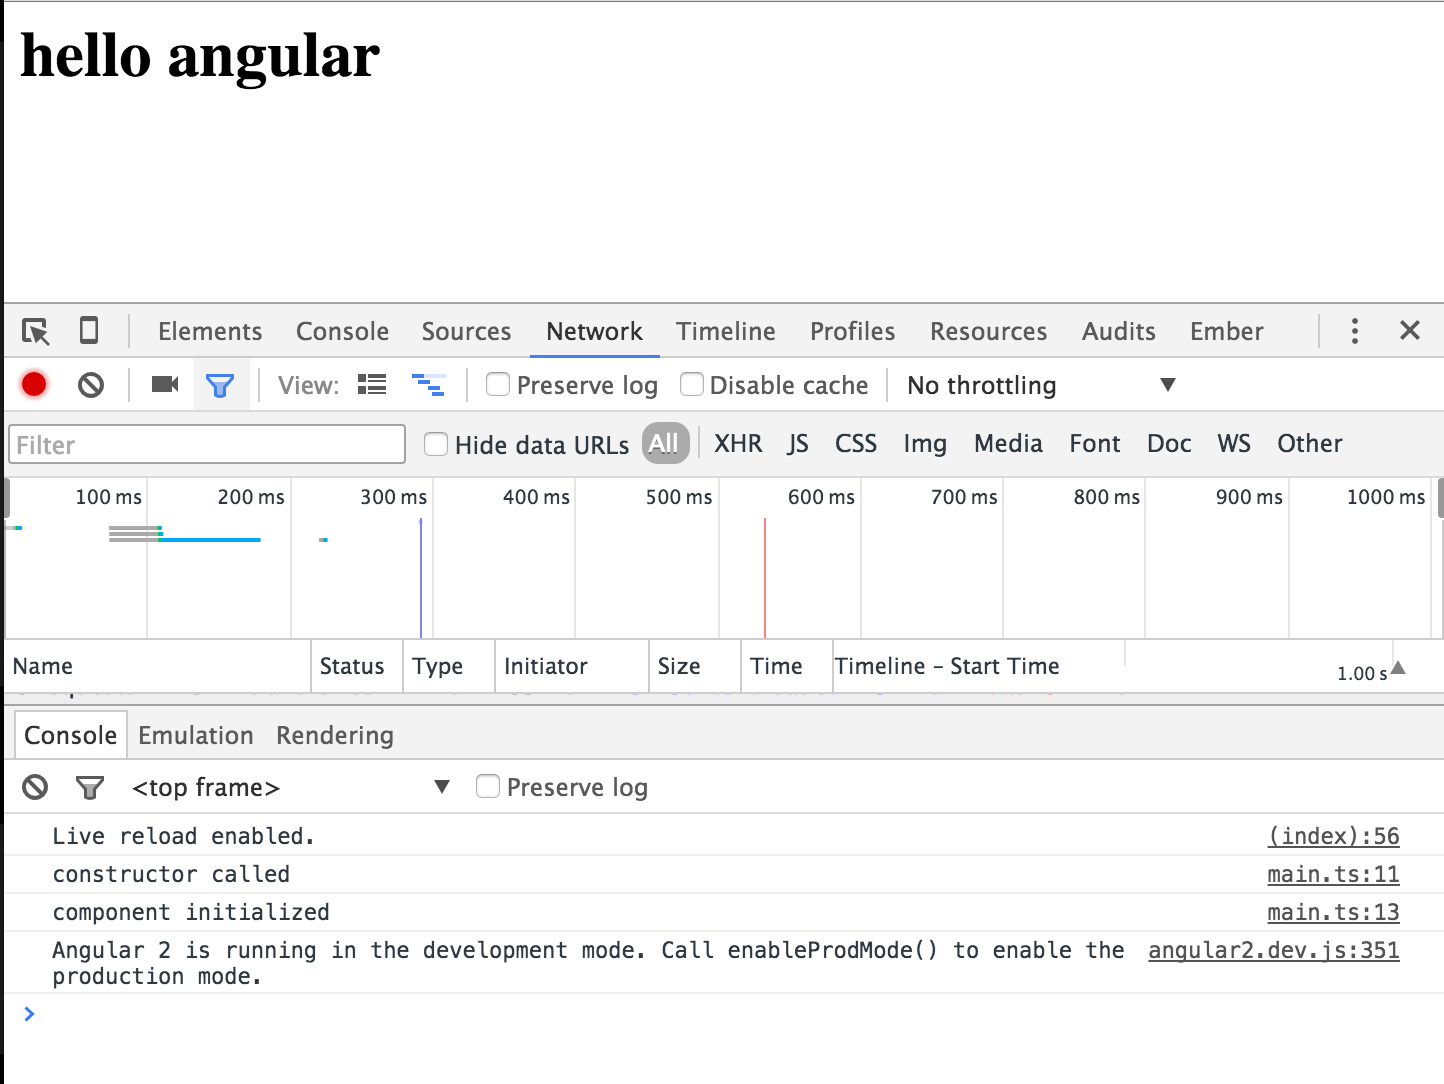
\includegraphics{images/hello-angular.png}
\caption{Running a basic component in the browser}
\end{figure}

\textbf{Debugging the component}

You can connect chrome's debugger to VSCode using the chrome debugger
extension for Visual Studio Code. See the
\protect\hyperlink{debugging-app-from-vscode}{Debugging App from VSCode}
section in case you missed to install it. But, assuming that you have
the extension installed, you can debug your app from VSCode. In order to
do that, we need to create a \texttt{launch.json} file in the
\texttt{.vscode} folder:

\begin{verbatim}
touch .vscode/launch.json
\end{verbatim}

After you created the file, put in the following configuration in the
file:

\begin{Shaded}
\begin{Highlighting}[numbers=left,,]
\FunctionTok{\{}
  \DataTypeTok{"version"}\FunctionTok{:} \StringTok{"0.1.0"}\FunctionTok{,}
  \DataTypeTok{"configurations"}\FunctionTok{:} \OtherTok{[}
    \FunctionTok{\{}
      \DataTypeTok{"name"}\FunctionTok{:} \StringTok{"Launch Chrome Debugger"}\FunctionTok{,}
      \DataTypeTok{"type"}\FunctionTok{:} \StringTok{"chrome"}\FunctionTok{,}
      \DataTypeTok{"request"}\FunctionTok{:} \StringTok{"launch"}\FunctionTok{,}
      \DataTypeTok{"url"}\FunctionTok{:} \StringTok{"http://127.0.0.1:8080/"}\FunctionTok{,}
      \DataTypeTok{"sourceMaps"}\FunctionTok{:} \KeywordTok{true}\FunctionTok{,}
      \DataTypeTok{"webRoot"}\FunctionTok{:} \StringTok{"."}\FunctionTok{,}
      \DataTypeTok{"runtimeExecutable"}\FunctionTok{:} \StringTok{"/Applications/Google Chrome.app/Contents/MacOS/Google Chrome"}\FunctionTok{,}
      \DataTypeTok{"runtimeArgs"}\FunctionTok{:} \OtherTok{[}
        \StringTok{"--remote-debugging-port=9222"}\OtherTok{,}
        \StringTok{"--incognito"}
      \OtherTok{]}
    \FunctionTok{\}}
  \OtherTok{]}
\FunctionTok{\}}
\end{Highlighting}
\end{Shaded}

Before running the debugger:

\begin{itemize}
\tightlist
\item
  Make sure that all instances of chrome are closed. It makes it easier
  to run the debugger from VSCode itself.
\item
  Make sure that the \texttt{runtimeExecutable} path is valid. This
  value would be different depending on your OS.
\item
  Make sure that the \texttt{url} value is valid as well. The
  \texttt{url} value has to match the path that you see when you run a
  server serving the files.
\item
  Set a breakpoint on a line in \texttt{main.ts} file and then run the
  debugger under the debugger tab.
\end{itemize}

In order to run the debugger, select \texttt{Launch\ Chrome\ Debugger}
in the dropdown under the debugger tab and either click on the play icon
or hit F5 on the keyboard. After that, an instance of Chrome should be
opened in incognito mode. In order to trigger the debugger just refresh
the page and you should be able to see the debugger pausing in VSCode.
If everything is set up correctly you should be able to see something
like the following screenshot:

\begin{figure}[htbp]
\centering
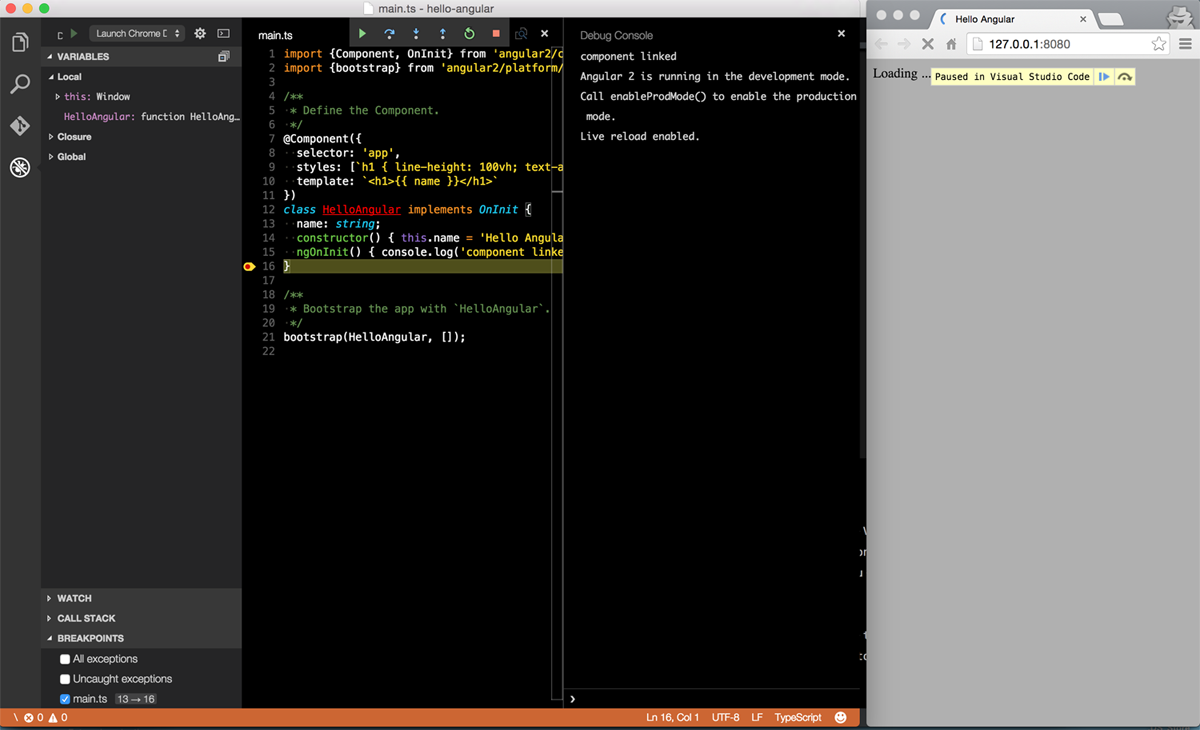
\includegraphics{images/run-debugger.png}
\caption{Debugging the app with Chrome Debugger in VSCode}
\end{figure}

\subsubsection{Component Inputs}\label{component-inputs}

\begin{itemize}
\tightlist
\item
  You can pass data to a component.
\item
  You can either use the \texttt{inputs} array on a component or
  annotate an instance variable with the \texttt{Input} decorator
\item
  Once you specify the inputs to your component, they become available
  in the \texttt{ngOnInit} method
\item
  You can implement the \texttt{ngOnInit} and access the input instance
  variables
\item
  You can use the \texttt{{[}propname{]}="data"} to set the
  \texttt{propname} to whatever \texttt{data} evaluates to
\item
  Note that if you set
  \texttt{{[}propname{]}="\textquotesingle{}data\textquotesingle{}"},
  \texttt{propname} will be set to the literal \texttt{data} string
\end{itemize}

\textbf{Project files}

The project files for this section are in
\href{https://github.com/aminmeyghani/angular2-intro/tree/master/project-files/angular-examples/component-input}{angular2-intro/project-files/angular-examples/component-input}.

\textbf{Getting Started}

In order to demonstrate component inputs, we are going to create a
\texttt{user} component and pass \texttt{name}, \texttt{lastName}, and
\texttt{userId} to it. So our final html tag would look something like
the following:

\begin{Shaded}
\begin{Highlighting}[numbers=left,,]
\KeywordTok{<user}\OtherTok{ name=}\StringTok{"Tom"}\OtherTok{ lastName=}\StringTok{"Johnson"}\OtherTok{ uesrId=}\StringTok{"1"}\KeywordTok{></user>}
\end{Highlighting}
\end{Shaded}

And the template for the component will be:

\begin{Shaded}
\begin{Highlighting}[numbers=left,,]
\KeywordTok{<h1>}\NormalTok{Hello, \{\{ name \}\} \{\{ lastName \}\}, id: \{\{ userId \}\}}\KeywordTok{</h1>}
\end{Highlighting}
\end{Shaded}

which would output: \texttt{Hello,\ Tom\ Johnson\ id:\ 1}.

To get started, let's define the \texttt{User} component:

\begin{Shaded}
\begin{Highlighting}[numbers=left,,]
\FunctionTok{@Component}\NormalTok{(\{}
  \NormalTok{selector: 'user',}
  \NormalTok{template: '<h1>Hello, \{\{ name \}\} \{\{ lastName \}\} id: \{\{ userId \}\}</h1>',}
  \NormalTok{inputs: ['name', 'lastName', 'userId'] }\CommentTok{// <- specifying the inputs to the `User` component}
\NormalTok{\})}
\KeywordTok{class} \NormalTok{User \{\}}
\end{Highlighting}
\end{Shaded}

\begin{itemize}
\tightlist
\item
  On line 4 we are defining the inputs as an array of strings
\end{itemize}

Then, we are going to use the \texttt{User} component inside our app's
template:

\begin{Shaded}
\begin{Highlighting}[numbers=left,,]
\FunctionTok{@Component}\NormalTok{(\{}
  \NormalTok{selector: 'app',}
  \NormalTok{template: `<user name=}\StringTok{"Tom"} \NormalTok{lastName=}\StringTok{"Johnson"} \NormalTok{uesrId=}\StringTok{"1"}\NormalTok{></user>`}
\NormalTok{\})}
\KeywordTok{class} \NormalTok{Root \{\}}
\end{Highlighting}
\end{Shaded}

because we are using the \texttt{User} component in the app, we need to
register it with the app by adding \texttt{User} class to the list of
\texttt{directives} of the app component:

\begin{Shaded}
\begin{Highlighting}[numbers=left,,]
\FunctionTok{@Component}\NormalTok{(\{}
  \NormalTok{selector: 'app',}
  \NormalTok{template: `<user name=}\StringTok{"Tom"} \NormalTok{lastName=}\StringTok{"Johnson"} \NormalTok{userId=}\StringTok{"1"}\NormalTok{></user>`,}
  \NormalTok{directives: [User] }\CommentTok{// <- register the component}
\NormalTok{\})}
\KeywordTok{class} \NormalTok{Root \{\}}
\end{Highlighting}
\end{Shaded}

and at the end we need to bootstrap the app:

\begin{Shaded}
\begin{Highlighting}[numbers=left,,]
\FunctionTok{bootstrap}\NormalTok{(Root, [])}
\end{Highlighting}
\end{Shaded}

Now, notice that instead of adding the inputs to the \texttt{inputs}
array, we could have decorated the instance variables with the
\texttt{@Input} decorator:

\begin{Shaded}
\begin{Highlighting}[numbers=left,,]
\KeywordTok{import \{Input\} from 'angular2/core';} \CommentTok{// <- importing the Input decorator}
\FunctionTok{@Component}\NormalTok{(\{}
  \NormalTok{selector: 'user',}
  \NormalTok{template: '<h1>Hello, \{\{ name \}\} \{\{ lastName \}\} id: \{\{ userId \}\}</h1>'}
  \CommentTok{// <- removing the inputs array.}
\NormalTok{\})}
\KeywordTok{class} \NormalTok{User \{}
  \FunctionTok{@Input}\NormalTok{() }\KeywordTok{private} \NormalTok{name: string;}
  \FunctionTok{@Input}\NormalTok{() }\KeywordTok{private} \NormalTok{lastName: string;}
  \FunctionTok{@Input}\NormalTok{() }\KeywordTok{private} \NormalTok{userId: number;}
\NormalTok{\}}
\end{Highlighting}
\end{Shaded}

\textbf{Binding Data to Properties}

Now, let's see how we can bind to a property from another component. For
this example, we are going to continue with our \texttt{User} component
and create a new component called \texttt{Permission}. Then we are going
to use the the \texttt{Permission} component inside the \texttt{User}
component and set the \texttt{uid} of \texttt{Permission} by the
\texttt{userId} of the \texttt{User}.

The \texttt{Permission} component is defined as follows:

\begin{Shaded}
\begin{Highlighting}[numbers=left,,]
\FunctionTok{@Component}\NormalTok{(\{}
  \NormalTok{selector: 'permission',}
  \NormalTok{template: '<h2> Restriction is: \{\{ restriction \}\}'}
\NormalTok{\})}
\KeywordTok{class} \NormalTok{Permission \{}
  \FunctionTok{@Input}\NormalTok{() }\KeywordTok{private} \NormalTok{uid: string;}
  \KeywordTok{private} \NormalTok{restriction: string;}
  \FunctionTok{constructor}\NormalTok{() \{}
    \KeywordTok{this}\NormalTok{.}\FunctionTok{restriction} \NormalTok{= 'none';}
  \NormalTok{\}}
  \FunctionTok{ngOnInit}\NormalTok{() \{}
    \KeywordTok{this}\NormalTok{.}\FunctionTok{restriction} \NormalTok{= }\KeywordTok{this}\NormalTok{.}\FunctionTok{uid} \NormalTok{=== '}\DecValTok{1}\NormalTok{' ? 'admin' : 'normal';}
  \NormalTok{\}}
\NormalTok{\}}
\end{Highlighting}
\end{Shaded}

\begin{itemize}
\tightlist
\item
  On line 6 we are defining \texttt{uid} to be an input instance
  variable. It's value is set from outside.
\item
  In the constructor we are setting a default value for the restriction.
\item
  Then in the \texttt{ngOnInit} hook, we are evaluating the value of
  \texttt{restriction} based on the given id provided by other
  components, in this case the \texttt{User} component
\item
  In this silly example, if the passed id is \texttt{1}, we will set the
  \texttt{restriction} to \texttt{admin}, otherwise we set it to
  \texttt{normal}.
\end{itemize}

then we are going to register the \texttt{Permission} component with the
\texttt{User} component so that we can use it in the \texttt{User}
template:

\begin{Shaded}
\begin{Highlighting}[numbers=left,,]
\FunctionTok{@Component}\NormalTok{(\{}
  \NormalTok{selector: 'user',}
  \CommentTok{///...}
  \NormalTok{directives: [Permission] }\CommentTok{// <-}
\NormalTok{\})}
\KeywordTok{class} \NormalTok{User \{\}}
\end{Highlighting}
\end{Shaded}

then we can update the \texttt{User} template to include the
\texttt{Permission}:

\begin{Shaded}
\begin{Highlighting}[numbers=left,,]
\FunctionTok{@Component}\NormalTok{(\{}
  \NormalTok{selector: 'user',}
  \NormalTok{template: `}
  \NormalTok{<h1>Hello, \{\{ name \}\} \{\{ lastName \}\}, id: \{\{ userId\}\}</h1>}
  \NormalTok{<div>}
    \NormalTok{<permission [uid]=}\StringTok{"userId"}\NormalTok{></permission>}
  \NormalTok{</div>}
  \NormalTok{`,}
  \NormalTok{inputs: ['name', 'lastName', 'userId'],}
  \NormalTok{directives: [Permission]}
\NormalTok{\})}
\KeywordTok{class} \NormalTok{User \{\}}
\end{Highlighting}
\end{Shaded}

\begin{itemize}
\tightlist
\item
  Note that on line 6 we are setting the \texttt{uid} of
  \texttt{Permission} by \texttt{userId} available from the
  \texttt{User} component.
\end{itemize}

If you run the app you should see the following printed to the page:

\begin{figure}[htbp]
\centering
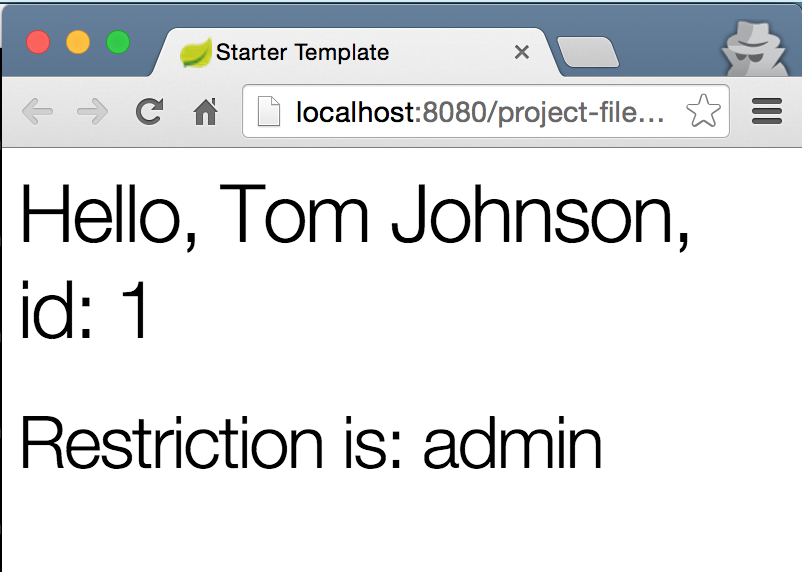
\includegraphics{images/input-cmp.png}
\caption{Input to components}
\end{figure}

\subsubsection{Binding to DOM
Properties}\label{binding-to-dom-properties}

In addition to custom properties, you can bind to DOM properties. Below
are some examples:

\textbf{Binding to \texttt{style}}

We can bind to the style property of DOM nodes. In the example below, if
the value of \texttt{isDone} is true, we set the
\texttt{style.textDecoration} to \texttt{line-through}, otherwise we
won't set it to anything

\begin{Shaded}
\begin{Highlighting}[numbers=left,,]
\KeywordTok{<div} \ErrorTok{[style.textDecoration]}\OtherTok{=}\StringTok{"isDone ? 'line-through' : ''"}\KeywordTok{>} \NormalTok{Todo Item }\KeywordTok{</div>}
\end{Highlighting}
\end{Shaded}

\textbf{Binding to \texttt{class}}

In addition to the \texttt{style} property, we can also bind to the
\texttt{class} property. In the example below, we are setting the class
name to ``collapsed'' if the \texttt{isCollapsed} value is true and
\texttt{expanded} if the the value is false:

\begin{Shaded}
\begin{Highlighting}[numbers=left,,]
\KeywordTok{<div} \ErrorTok{[className]}\OtherTok{=}\StringTok{"isCollapsed ? 'collapsed' : 'expanded'"}\KeywordTok{>}\NormalTok{Element}\KeywordTok{</div>}
\end{Highlighting}
\end{Shaded}

\textbf{Binding to `hidden'}

You can bind to the hidden property of a DOM node and show or hide the
element. In the example below, we are hiding the element if the
\texttt{isVisible} value is true:

\begin{Shaded}
\begin{Highlighting}[numbers=left,,]
\KeywordTok{<div} \ErrorTok{[hidden]}\OtherTok{=}\StringTok{"isVisible"}\KeywordTok{>}\NormalTok{To Hide element}\KeywordTok{</div>}
\end{Highlighting}
\end{Shaded}

\textbf{Binding to \texttt{textContent}}

We can bind to the \texttt{textContent} property and set the text
content of a node. In the example below, we are setting the text content
by reading the value of an input:

\begin{Shaded}
\begin{Highlighting}[numbers=left,,]
\KeywordTok{<div} \ErrorTok{[textContent]}\OtherTok{=}\StringTok{"textValue"}\KeywordTok{></div>}
\KeywordTok{<input}\OtherTok{ type=}\StringTok{"text"} \ErrorTok{#contentInput}\KeywordTok{>}
\KeywordTok{<button} \ErrorTok{(click)}\OtherTok{=}\StringTok{"setTextContent()"}\KeywordTok{>}\NormalTok{Set Text Content}\KeywordTok{</button>}
\end{Highlighting}
\end{Shaded}

\subsubsection{Component Output/Events}\label{component-outputevents}

\begin{itemize}
\tightlist
\item
  Events can be emitted from components. These events can be either
  custom or they could be DOM events
\item
  The syntax is \texttt{(eventname)="fn()"} where \texttt{eventname} is
  the name of the event and \texttt{fn} is the handler function
\item
  The handler function is called when the event is fired
\item
  For example, if you want to handle a click event you can do:
  \texttt{(click)="handler()"}. In this case the \texttt{hander} is
  called whenever the click event is fired off
\item
  You can use Angular's \texttt{EventEmitter} to fire off custom events
\end{itemize}

\paragraph{Custom Output Events}\label{custom-output-events}

\textbf{Project Files}

The project files for this section are in
\href{https://github.com/aminmeyghani/angular2-intro/tree/master/project-files/angular-examples/component-output-events}{angular2-intro/project-files/angular-examples/component-output-events}.

\textbf{Final Result}

The goal of this section is to show you how to create a component that
contains a button that when is clicked, calls a handler defined by the
component's class. The final html will look like the following:

\begin{Shaded}
\begin{Highlighting}[numbers=left,,]
\KeywordTok{<p>}\NormalTok{Value: \{\{ value \}\}}\KeywordTok{</p>}
\KeywordTok{<button} \ErrorTok{(click)}\OtherTok{=}\StringTok{addOne()}\KeywordTok{>}\NormalTok{Add +}\KeywordTok{</button>}
\end{Highlighting}
\end{Shaded}

That idea is very simple: every time we click on the button we want to
increment the value by one. In addition to that, we want to be able to
hook into a custom event and run the \texttt{addOne} method whenever the
event is fired:

\begin{Shaded}
\begin{Highlighting}[numbers=left,,]
\KeywordTok{<p>}\NormalTok{Value: \{\{ value \}\}}\KeywordTok{</p>}
\KeywordTok{<span}\OtherTok{ adder-auto} \ErrorTok{(myevent)}\OtherTok{=}\StringTok{addOne()}\KeywordTok{>}\NormalTok{adding ...}\KeywordTok{</span>}
\end{Highlighting}
\end{Shaded}

\textbf{Getting Started}

Let's get started by defining our \texttt{Adder} component:

\begin{Shaded}
\begin{Highlighting}[numbers=left,,]
\FunctionTok{@Component}\NormalTok{(\{}
  \NormalTok{selector: 'adder',}
  \NormalTok{template:`}
  \NormalTok{<p>Value: \{\{ value \}\}</p>}
  \NormalTok{<}\FunctionTok{button} \NormalTok{(click)=}\FunctionTok{addOne}\NormalTok{()>Add +</button>}
  \NormalTok{`}
\NormalTok{\})}
\KeywordTok{class} \NormalTok{Adder \{}
  \KeywordTok{private} \NormalTok{value: number;}
  \FunctionTok{constructor}\NormalTok{() \{}
    \KeywordTok{this}\NormalTok{.}\FunctionTok{value} \NormalTok{= }\DecValTok{0}\NormalTok{;}
  \NormalTok{\}}
  \FunctionTok{addOne}\NormalTok{() \{}
  \KeywordTok{this}\NormalTok{.}\FunctionTok{value} \NormalTok{+= }\DecValTok{1}\NormalTok{;}
  \NormalTok{console.}\FunctionTok{log}\NormalTok{(}\KeywordTok{this}\NormalTok{.}\FunctionTok{value}\NormalTok{);}
  \NormalTok{\}}
\NormalTok{\}}
\end{Highlighting}
\end{Shaded}

Now, we are just going to register \texttt{Adder} with our root
component:

\begin{Shaded}
\begin{Highlighting}[numbers=left,,]
\FunctionTok{@Component}\NormalTok{(\{}
  \NormalTok{selector: 'app',}
  \NormalTok{directives: [Adder],}
  \NormalTok{template: '<adder></adder>'}
\NormalTok{\})}
\KeywordTok{class} \NormalTok{App \{\}}
\end{Highlighting}
\end{Shaded}

after you bootstrap the app and run it you should be able to see a
button that when clicked increments the value by one.

\textbf{Using EventEmitter}

Now, let's see how we can use the \texttt{EventEmitter} to increment the
value by one every time a custom event is fired every second. In order
to achieve that, we are going to create an attribute directive called
\texttt{AdderAuto}. Start by importing the \texttt{Directive} metadata
class:

\begin{Shaded}
\begin{Highlighting}[numbers=left,,]
\KeywordTok{import \{Directive\} from 'angular2/core';}
\end{Highlighting}
\end{Shaded}

and then define the selector for the directive:

\begin{Shaded}
\begin{Highlighting}[numbers=left,,]
\FunctionTok{@Directive}\NormalTok{(\{}
  \NormalTok{selector: '[adder-auto]'}
\NormalTok{\})}
\end{Highlighting}
\end{Shaded}

\begin{itemize}
\tightlist
\item
  \texttt{selector:\ \textquotesingle{}{[}adder-auto{]}\textquotesingle{}}
  means that angular will target any element that has the
  \texttt{adder-auto} attribute and will create an instance of the
  class. Now we need to define the class for our directive:
\end{itemize}

\begin{Shaded}
\begin{Highlighting}[numbers=left,,]
\KeywordTok{class} \NormalTok{AdderAuto \{}
  \CommentTok{// custom event definition}
\NormalTok{\}}
\end{Highlighting}
\end{Shaded}

In this class we need to define a custom event output hook. We are going
to call it \texttt{myevent}. The same way that you can hook into
\texttt{(click)}, we want to be able to use \texttt{(myevent)}. To
achieve that, we need to create an instance variable and decorate it
with the \texttt{Output} decorator:

\begin{Shaded}
\begin{Highlighting}[numbers=left,,]
\CommentTok{// -> importing `EventEmitter` and `Output` decorator.}
\KeywordTok{import \{EventEmitter, Output\} from 'angular2/core';}
\KeywordTok{class} \NormalTok{AdderAuto \{}
  \FunctionTok{@Output}\NormalTok{() myevent: EventEmitter<string>;}
  \FunctionTok{constructor}\NormalTok{() \{}
    \KeywordTok{this}\NormalTok{.}\FunctionTok{myevent} \NormalTok{= }\KeywordTok{new} \FunctionTok{EventEmitter}\NormalTok{();}
  \NormalTok{\}}
\NormalTok{\}}
\end{Highlighting}
\end{Shaded}

\begin{itemize}
\tightlist
\item
  If you notice, \texttt{myevent} is of type \texttt{EventEmitter} that
  emit events of type string
\item
  In the constructor we are creating an instance of
  \texttt{EventEmitter}. So now we can use \texttt{myevent} to emit
  events
\item
  We can use \texttt{setInterval} to emit event from our custom event
  every second
\end{itemize}

\begin{Shaded}
\begin{Highlighting}[numbers=left,,]
\KeywordTok{class} \NormalTok{AdderAuto \{}
  \FunctionTok{@Output}\NormalTok{() myevent: EventEmitter<string>;}
  \FunctionTok{constructor}\NormalTok{() \{}
    \KeywordTok{this}\NormalTok{.}\FunctionTok{myevent} \NormalTok{= }\KeywordTok{new} \FunctionTok{EventEmitter}\NormalTok{();}
    \FunctionTok{setInterval}\NormalTok{(()=> \{}\KeywordTok{this}\NormalTok{.}\FunctionTok{myevent}\NormalTok{.}\FunctionTok{emit}\NormalTok{('myevename')\}, }\DecValTok{1000}\NormalTok{);}
  \NormalTok{\}}
\NormalTok{\}}
\end{Highlighting}
\end{Shaded}

Now we can register \texttt{AdderAuto} with the \texttt{Adder} component
and run the \texttt{addOne} method every second:

\begin{Shaded}
\begin{Highlighting}[numbers=left,,]
\FunctionTok{@Component}\NormalTok{(\{}
  \NormalTok{selector: 'adder',}
  \NormalTok{...}
  \NormalTok{directives: [AdderAuto] }\CommentTok{// <- register `AdderAuto`}
\NormalTok{\})}
\end{Highlighting}
\end{Shaded}

and then we can update the template:

\begin{Shaded}
\begin{Highlighting}[numbers=left,,]
\KeywordTok{<p>}\NormalTok{Value: \{\{ value \}\}}\KeywordTok{</p>}
\KeywordTok{<button} \ErrorTok{(click)}\OtherTok{=}\StringTok{"addOne()"}\KeywordTok{>}\NormalTok{Add +}\KeywordTok{</button>}
\CommentTok{<!-- using the event. -->}
\KeywordTok{<h2>}\NormalTok{Using Emitter}\KeywordTok{</h2>}
\KeywordTok{<span}\OtherTok{ adder-auto} \ErrorTok{(myevent)}\OtherTok{=}\StringTok{"addOne($event)"}\KeywordTok{>} \NormalTok{EVENT: }\KeywordTok{</span>}
\end{Highlighting}
\end{Shaded}

\begin{itemize}
\tightlist
\item
  first we are adding the attribute directive \texttt{adder-auto} on the
  span
\item
  second, we are using the \texttt{myevent} hook and attaching
  \texttt{addOne} handler to it. This means that whenever the
  \texttt{myevent} event is triggered, run the \texttt{addOne} handler.
\end{itemize}

The \texttt{Adder} component now looks like the following with the
updated template:

\begin{Shaded}
\begin{Highlighting}[numbers=left,,]
\FunctionTok{@Component}\NormalTok{(\{}
  \NormalTok{selector: 'adder',}
  \NormalTok{template:`}
  \NormalTok{<p>Value: \{\{ value \}\}</p>}
  \NormalTok{<}\FunctionTok{button} \NormalTok{(click)=}\StringTok{"addOne()"}\NormalTok{>Add +</button>}
  \NormalTok{<h2>Using Emitter</h2>}
  \NormalTok{<span adder-}\FunctionTok{auto} \NormalTok{(myevent)=}\StringTok{"addOne($event)"}\NormalTok{> EVENT: </span>}
  \NormalTok{`,}
  \NormalTok{directives: [AdderAuto]}
\NormalTok{\})}
\end{Highlighting}
\end{Shaded}

Now if you run the code, you should be able to see the number
incrementing by one every second.

\paragraph{Binding to DOM Events}\label{binding-to-dom-events}

In addition to custom output events, we can bind to almost all of the
native DOM events. Below you can find some common events with examples:

\textbf{Inputs}

\begin{itemize}
\item
  \href{https://developer.mozilla.org/en-US/docs/Web/Events/keyup}{keyup}

\begin{Shaded}
\begin{Highlighting}[numbers=left,,]
\KeywordTok{<input}\OtherTok{ type=}\StringTok{"text"} \ErrorTok{#inputField2} \ErrorTok{(keyup)}\OtherTok{=}\StringTok{"setInputFieldValue2(inputField2.value)"}\KeywordTok{>}
\KeywordTok{<pre>} \NormalTok{\{\{ keyupValue \}\}}\KeywordTok{</pre>}
\end{Highlighting}
\end{Shaded}
\item
  \href{https://developer.mozilla.org/en-US/docs/Web/Events/input}{input}

\begin{Shaded}
\begin{Highlighting}[numbers=left,,]
\KeywordTok{<input}\OtherTok{ type=}\StringTok{"text"} \ErrorTok{#inputField} \ErrorTok{(input)}\OtherTok{=}\StringTok{"setInputFieldValue(inputField.value)"}\KeywordTok{>}
\KeywordTok{<pre>} \NormalTok{\{\{ inputValue \}\}}\KeywordTok{</pre>}
\end{Highlighting}
\end{Shaded}
\end{itemize}

\textbf{Mouse}

\begin{itemize}
\item
  \href{https://developer.mozilla.org/en-US/docs/Web/Events/click}{click}

\begin{Shaded}
\begin{Highlighting}[numbers=left,,]
\KeywordTok{<button} \ErrorTok{(click)}\OtherTok{=}\StringTok{"sayHello()"}\KeywordTok{>} \NormalTok{Say Hello! }\KeywordTok{</button>}
\KeywordTok{<pre>}\NormalTok{\{\{ hello \}\}}\KeywordTok{</pre>}
\end{Highlighting}
\end{Shaded}
\item
  \href{https://developer.mozilla.org/en-US/docs/Web/Events/dblclick}{dblclick}

\begin{Shaded}
\begin{Highlighting}[numbers=left,,]
\KeywordTok{<button} \ErrorTok{(dblclick)}\OtherTok{=}\StringTok{"sayDoubleHello()"}\KeywordTok{>} \NormalTok{Say Hello! }\KeywordTok{</button>}
\KeywordTok{<pre>}\NormalTok{\{\{ doubleHello \}\}}\KeywordTok{</pre>}
\end{Highlighting}
\end{Shaded}
\item
  \href{https://developer.mozilla.org/en-US/docs/Web/Events/mousedown}{mousedown}

\begin{Shaded}
\begin{Highlighting}[numbers=left,,]
\KeywordTok{<button} \ErrorTok{(mousedown)}\OtherTok{=}\StringTok{"sayDownHello()"}\KeywordTok{>}\NormalTok{Say Hello !}\KeywordTok{</button>}
\KeywordTok{<pre>}\NormalTok{\{\{ downHello \}\}}\KeywordTok{</pre>}
\end{Highlighting}
\end{Shaded}
\item
  \href{https://developer.mozilla.org/en-US/docs/Web/Events/mouseup}{mouseup}

\begin{Shaded}
\begin{Highlighting}[numbers=left,,]
\KeywordTok{<button} \ErrorTok{(mouseup)}\OtherTok{=}\StringTok{"sayUpHello()"}\KeywordTok{>}\NormalTok{Say Hello !}\KeywordTok{</button>}
\KeywordTok{<pre>}\NormalTok{\{\{ upHello \}\}}\KeywordTok{</pre>}
\end{Highlighting}
\end{Shaded}
\item
  \href{https://developer.mozilla.org/en-US/docs/Web/Events/mouseenter}{mouseenter}

\begin{Shaded}
\begin{Highlighting}[numbers=left,,]
\KeywordTok{<h2} \ErrorTok{(mouseenter)}\OtherTok{=}\StringTok{"sayEnterHello()"} \ErrorTok{(mouseleave)}\OtherTok{=}\StringTok{"clearEnterHello()"}\KeywordTok{>}\NormalTok{Mouseenter/leave}\KeywordTok{</h2>}
\KeywordTok{<pre>}\NormalTok{\{\{ enterHello \}\}}\KeywordTok{</pre>}
\end{Highlighting}
\end{Shaded}
\item
  \href{https://developer.mozilla.org/en-US/docs/Web/Events/mouseleave}{mouseleave}

\begin{Shaded}
\begin{Highlighting}[numbers=left,,]
\KeywordTok{<h2} \ErrorTok{(mouseenter)}\OtherTok{=}\StringTok{"sayEnterHello()"} \ErrorTok{(mouseleave)}\OtherTok{=}\StringTok{"clearEnterHello()"}\KeywordTok{>}\NormalTok{Mouseenter/leave}\KeywordTok{</h2>}
\KeywordTok{<pre>}\NormalTok{\{\{ enterHello \}\}}\KeywordTok{</pre>}
\end{Highlighting}
\end{Shaded}
\end{itemize}

\paragraph{Event Delegation/Bubbling}\label{event-delegationbubbling}

When an event is raised by an element, by default it bubbles up the html
hierarchy. For example, if you have a table and attached a click handler
to the table itself, you can catch the row that was clicked by only
attaching a single handler. This method is useful when you are dealing
with situations where you don't want to attach event handlers to every
elements, and you just want to attach one. Below is an example of event
delegation, detecting the row that was clicked on the table:

\begin{Shaded}
\begin{Highlighting}[numbers=left,,]
\KeywordTok{<pre>}\NormalTok{\{\{rowClicked\}\}}\KeywordTok{</pre>}

\KeywordTok{<table} \ErrorTok{(click)}\OtherTok{=}\StringTok{"catchBubbledEvent($event)"}\KeywordTok{>}
  \KeywordTok{<tr>}
    \KeywordTok{<td>}\NormalTok{1}\KeywordTok{</td>}
  \KeywordTok{</tr>}
  \KeywordTok{<tr>}
    \KeywordTok{<td>}\NormalTok{2}\KeywordTok{</td>}
  \KeywordTok{</tr>}
  \KeywordTok{<tr>}
    \KeywordTok{<td>}\NormalTok{3}\KeywordTok{</td>}
  \KeywordTok{</tr>}
  \KeywordTok{<tr>}
    \KeywordTok{<td>}\NormalTok{4}\KeywordTok{</td>}
  \KeywordTok{</tr>}
\KeywordTok{</table>}
\end{Highlighting}
\end{Shaded}

Notice how we have a single \texttt{click} handler only on the table
itself. The \texttt{\$event} is the bubbled event that we can catch to
do interesting stuff with. In this case we are just reading the
\texttt{textContent} from the target: \texttt{event.target.textContent}:

\begin{Shaded}
\begin{Highlighting}[numbers=left,,]
\FunctionTok{catchBubbledEvent}\NormalTok{(event) \{}
  \KeywordTok{this}\NormalTok{.}\FunctionTok{rowClicked} \NormalTok{= event.}\FunctionTok{target}\NormalTok{.}\FunctionTok{nodeName} \NormalTok{=== 'TD' ? event.}\FunctionTok{target}\NormalTok{.}\FunctionTok{textContent} \NormalTok{: '';}
\NormalTok{\}}
\end{Highlighting}
\end{Shaded}

In the method above we are checking if a \texttt{td} was clicked on. If
so, we set the \texttt{this.rowClicked} to the td's value, otherwise we
set it to an empty string.

\subsubsection{ViewChildren}\label{viewchildren}

\begin{itemize}
\tightlist
\item
  The children elements located inside of its template of a component
  are called
\item
  Metadata classes: \texttt{@ViewChildren}, \texttt{@ViewChild}
\end{itemize}

\textbf{TODO}

\subsubsection{ContentChildren}\label{contentchildren}

\begin{itemize}
\tightlist
\item
  Elements used between the opening and closing tags of the host element
  of a given component
\item
  Metadata classes: \texttt{@ContentChildren}, \texttt{@ContentChild}
\end{itemize}

\textbf{TODO}

\subsubsection{ViewProviders}\label{viewproviders}

\textbf{TODO}

\subsubsection{Providers}\label{providers}

\textbf{TODO}

\subsection{Directives}\label{directives}

\begin{itemize}
\tightlist
\item
  Directives and components hand-in-hand are the fundamental building
  blocks of any Angular app
\item
  Directives are components without templates. Conversely, components
  are directives without templates
\item
  Directives allow you to attach behavior to elements in the DOM
\item
  A directive is defined using the \texttt{@directive} decorator
\item
  There are three types of directives in Angular:

  \begin{itemize}
  \tightlist
  \item
    Structural
  \item
    Attribute
  \item
    Components
  \end{itemize}
\item
  Evey directive metadata, has the following options:

  \begin{itemize}
  \tightlist
  \item
    selector
  \item
    host
  \item
    \ldots{}
  \end{itemize}
\item
  The \texttt{selector} attribute uses a css selector to find the
  element. However, parent-child relationship selectors are not
  supported
\item
  You can use the following possible selectors:

  \begin{itemize}
  \tightlist
  \item
    \texttt{element}
  \item
    \texttt{{[}attribute{]}}
  \item
    \texttt{.classname}
  \item
    \texttt{:not()}
  \item
    \texttt{.some-class:not(div)}
  \end{itemize}
\item
  The \texttt{host} option defines:

  \begin{itemize}
  \tightlist
  \item
    Property bindings
  \item
    Event handlers
  \item
    attributes
  \end{itemize}
\end{itemize}

\textbf{TODO}(other decorator options)

\subsubsection{Web Components Basics}\label{web-components-basics}

Web Components are made up four specifications:

\begin{itemize}
\tightlist
\item
  Custom Elements: enabling custom html tags
\item
  Shadow DOM: enabling isolation for custom elements
\item
  HTML Templates: enabling to define html template fragments
\item
  HTML Imports: enabling html fragment imports
\end{itemize}

\textbf{Custom Elements}

\textbf{TODO}

\textbf{Shadow DOM}

\begin{itemize}
\tightlist
\item
  Enables a node to express three subtrees:

  \begin{itemize}
  \tightlist
  \item
    Light DOM: visible DOM notes inside the custom element tag/DOM
    supplied by the consumer
  \item
    Shadow DOM: private to the element and hidden from others and
    attached to the element's shadow root
  \item
    Composed DOM: Rendered by the browser by distributing the light DOM
    into the Shadow DOM
  \item
    \emph{Logical DOM} = Light DOM + Shadow DOM. The developer interacts
    with this layer
  \end{itemize}
\end{itemize}

\textbf{TODO}

\textbf{HTML Templates}

\textbf{TODO}

\textbf{HTML Imports}

\textbf{TODO}

\subsubsection{host}\label{host}

\textbf{TODO}

\subsubsection{selector}\label{selector}

\textbf{TODO}

\subsubsection{Attribute Directives}\label{attribute-directives}

\begin{itemize}
\tightlist
\item
  The Attribute directive changes the appearance or behavior of an
  element.
\item
  Angular has several built-in attribute directives, namely
  \texttt{NgClass} and \texttt{NgStyle}
\item
  It is a good idea to prefix your directives with a prefix. You cannot
  use the \texttt{ng} prefix since it's already used by Angular.
\item
  When you apply the attribute directive to an element, the element will
  be knownn as the \textbf{host}.
\item
  For example, if you had a directive called \texttt{my-directive} and
  applied it in
  \texttt{\textless{}div\ class="hello"\textgreater{}\ \textless{}span\ my-directive\textgreater{}\ ...\ \textless{}/span\textgreater{}\ \textless{}/div\textgreater{}},
  the \texttt{span} would be the \textbf{host}.
\end{itemize}

\textbf{TODO} (writing a custom attribute directive)

\begin{Shaded}
\begin{Highlighting}[numbers=left,,]
\FunctionTok{@Directive}\NormalTok{(\{}
  \NormalTok{selector: '[simple-directive]',}
  \NormalTok{host: \{}
    \NormalTok{'(mouseleave)': '}\FunctionTok{onMouseLeave}\NormalTok{()',}
    \NormalTok{'(click)': '}\FunctionTok{onClick}\NormalTok{()',}
    \NormalTok{'[hidden]': 'isHidden',}
    \NormalTok{'[}\KeywordTok{class}\NormalTok{.}\FunctionTok{done}\NormalTok{]': 'isDone',}
    \NormalTok{'role': 'button'}
  \NormalTok{\}}
\NormalTok{\})}
\KeywordTok{class} \NormalTok{SimpleDirective }\KeywordTok{implements} \NormalTok{OnInit \{}
  \FunctionTok{@Input}\NormalTok{() }\KeywordTok{private} \NormalTok{color: string}
  \FunctionTok{@Output}\NormalTok{() myevent: EventEmitter<string>;}
  \KeywordTok{private} \NormalTok{isHidden: }\DataTypeTok{boolean} \NormalTok{= }\KeywordTok{false}\NormalTok{;}
  \KeywordTok{private} \NormalTok{isDone: }\DataTypeTok{boolean} \NormalTok{= }\KeywordTok{false}\NormalTok{;}
  \KeywordTok{private} \NormalTok{defaultColor:string = 'magenta';}
  \KeywordTok{private} \NormalTok{elm: any;}

  \FunctionTok{constructor}\NormalTok{(}\KeywordTok{private} \NormalTok{elmRef: ElementRef, }\KeywordTok{private} \NormalTok{renderer: Renderer) \{}
    \KeywordTok{this}\NormalTok{.}\FunctionTok{elm} \NormalTok{= elmRef.}\FunctionTok{nativeElement}\NormalTok{;}
    \KeywordTok{this}\NormalTok{.}\FunctionTok{myevent} \NormalTok{= }\KeywordTok{new} \FunctionTok{EventEmitter}\NormalTok{();}
    \FunctionTok{setInterval}\NormalTok{(() => \{}\KeywordTok{this}\NormalTok{.}\FunctionTok{myevent}\NormalTok{.}\FunctionTok{emit}\NormalTok{('myevename')\}, }\DecValTok{1000}\NormalTok{);}
  \NormalTok{\}}
  \FunctionTok{ngOnInit}\NormalTok{() \{}
    \KeywordTok{this}\NormalTok{.}\FunctionTok{defaultColor} \NormalTok{= }\KeywordTok{this}\NormalTok{.}\FunctionTok{color} \NormalTok{|| }\KeywordTok{this}\NormalTok{.}\FunctionTok{defaultColor}\NormalTok{;}
    \KeywordTok{this}\NormalTok{.}\FunctionTok{setColor}\NormalTok{(}\KeywordTok{this}\NormalTok{.}\FunctionTok{color} \NormalTok{|| }\KeywordTok{this}\NormalTok{.}\FunctionTok{defaultColor}\NormalTok{);}
  \NormalTok{\}}
  \KeywordTok{private} \FunctionTok{setColor}\NormalTok{(color: string) \{}
    \KeywordTok{this}\NormalTok{.}\FunctionTok{renderer}\NormalTok{.}\FunctionTok{setElementStyle}\NormalTok{(}\KeywordTok{this}\NormalTok{.}\FunctionTok{elm}\NormalTok{, 'color', color);}
  \NormalTok{\}}
  \NormalTok{set }\FunctionTok{setIsHidden}\NormalTok{(state) \{ }\KeywordTok{this}\NormalTok{.}\FunctionTok{isHidden} \NormalTok{= state; \}}
  \NormalTok{set }\FunctionTok{setIsDone}\NormalTok{(state) \{ }\KeywordTok{this}\NormalTok{.}\FunctionTok{isDone} \NormalTok{= state; \}}

  \FunctionTok{onMouseLeave}\NormalTok{() \{ }\KeywordTok{this}\NormalTok{.}\FunctionTok{setColor}\NormalTok{(}\KeywordTok{this}\NormalTok{.}\FunctionTok{defaultColor}\NormalTok{); \}}
  \FunctionTok{onClick}\NormalTok{() \{ }\KeywordTok{this}\NormalTok{.}\FunctionTok{setColor}\NormalTok{('orange') \}}
\NormalTok{\}}
\end{Highlighting}
\end{Shaded}

\textbf{selector} TODO: details

\textbf{host} TODO: details

\textbf{Input} TODO: details

\textbf{Output} TODO: details

\textbf{ElementRef} TODO: details**

\textbf{Renderer} TODO: details**

\subsubsection{Structural Directives}\label{structural-directives}

\begin{itemize}
\tightlist
\item
  The Structural directive changes the DOM layout by adding and removing
  DOM elements
\item
  Angular has several built-in structural directives, namely
  \texttt{NgIf}, \texttt{NgSwitch}, and \texttt{NgFor}
\item
  When working with structural directives, we should ask ourselves to
  think carefully about the consequences of adding and removing elements
  and of creating and destroying components
\item
  Angular uses the html5 \texttt{\textless{}template\textgreater{}} tag
  to add or remove DOM elements
\item
  By default, Angular replaces
  \texttt{\textless{}template\textgreater{}} with
  \texttt{\textless{}script\textgreater{}} tag if no behavior is
  attached
\item
  The \texttt{*} before a directive name is a shorthand for including
  the directive content in the
  \texttt{\textless{}template\textgreater{}} tag
\item
  Below you can see the built-in \texttt{NgIf} directive with and
  without the asterisks \texttt{*}:
\end{itemize}

\textbf{With \texttt{*}}

\begin{Shaded}
\begin{Highlighting}[numbers=left,,]
\KeywordTok{<p} \ErrorTok{*ngIf}\OtherTok{=}\StringTok{"condition"}\KeywordTok{></p>}
\end{Highlighting}
\end{Shaded}

\textbf{Without \texttt{*}}

\begin{Shaded}
\begin{Highlighting}[numbers=left,,]
\KeywordTok{<template} \ErrorTok{[ngIf]}\OtherTok{=}\StringTok{"condition"}\KeywordTok{>}
  \KeywordTok{<p></p>}
\KeywordTok{</template>}
\end{Highlighting}
\end{Shaded}

Notice how the \texttt{\textless{}p\textgreater{}} tag is wrapped with a
\texttt{\textless{}template\textgreater{}} and the condition is bound to
the \texttt{{[}ngIf{]}} property of the directive

\textbf{TODO} (writing a custom structural directive)

\begin{Shaded}
\begin{Highlighting}[numbers=left,,]
\FunctionTok{@Directive}\NormalTok{(\{}
  \NormalTok{selector: '[myUnless]'}
\NormalTok{\})}
\KeywordTok{class} \NormalTok{UnlessDirective \{}

  \FunctionTok{constructor}\NormalTok{(}
    \KeywordTok{private} \NormalTok{tRef: TemplateRef,}
    \KeywordTok{private} \NormalTok{vContainer: ViewContainerRef}
  \NormalTok{) \{ \}}

  \FunctionTok{@Input}\NormalTok{() set }\FunctionTok{myUnless}\NormalTok{(condition: }\DataTypeTok{boolean}\NormalTok{) \{}
    \KeywordTok{if} \NormalTok{(!condition) \{}
      \KeywordTok{this}\NormalTok{.}\FunctionTok{vContainer}\NormalTok{.}\FunctionTok{createEmbeddedView}\NormalTok{(}\KeywordTok{this}\NormalTok{.}\FunctionTok{tRef}\NormalTok{);}
    \NormalTok{\} }\KeywordTok{else} \NormalTok{\{}
      \KeywordTok{this}\NormalTok{.}\FunctionTok{vContainer}\NormalTok{.}\FunctionTok{clear}\NormalTok{();}
    \NormalTok{\}}
  \NormalTok{\}}
\NormalTok{\}}
\end{Highlighting}
\end{Shaded}

\textbf{TemplateRef}: TODO: details

\textbf{ViewContainerRef}: TODO: details

\textbf{\texttt{@Input()\ set\ myUnless(condition:\ boolean)\ \{\}}}:
TODO: details

\subsubsection{Built-in Directives}\label{built-in-directives}

Angular has a couple of useful built-in directives.

\textbf{TODO}(Note on directive names, docs and template usage)

\paragraph{\texorpdfstring{\texttt{NgClass}}{NgClass}}\label{ngclass}

\begin{itemize}
\tightlist
\item
  \texttt{import\ \{NgClass\}\ from\ \textquotesingle{}angular2/common\textquotesingle{};},
  \texttt{directives:\ {[}NgClass{]}}
\item
  Template Usage:
  \texttt{\textless{}div\ class="button"\ {[}ngClass{]}="\{active:\ isActive,\ disabled:\ !isActive\}"}
\end{itemize}

\textbf{Note} that we are using \texttt{ngClass} in the template, but
not \texttt{NgClass}

\paragraph{\texorpdfstring{\texttt{NgIf}}{NgIf}}\label{ngif}

\textbf{Usage}

\begin{Shaded}
\begin{Highlighting}[numbers=left,,]
\KeywordTok{<div} \ErrorTok{*ngIf}\OtherTok{=}\StringTok{"isDone"}\KeywordTok{>}\NormalTok{\{\{ list \}\}}\KeywordTok{</div>}
\end{Highlighting}
\end{Shaded}

or in long-hand form:

\begin{Shaded}
\begin{Highlighting}[numbers=left,,]
\KeywordTok{<template>}
  \KeywordTok{<div} \ErrorTok{[ngIf]}\OtherTok{=}\StringTok{"isDone"}\KeywordTok{>}\NormalTok{\{\{ list \}\}}\KeywordTok{</div>}
\KeywordTok{</template>}
\end{Highlighting}
\end{Shaded}

\textbf{Details}

From the docs: ``The ngIf directive does not hide the element. Using
browser developer tools we can see that, when the condition is true, the
top paragraph is in the DOM and the bottom disused paragraph is
completely absent from the DOM! In its place are empty
\texttt{\textless{}script\textgreater{}} tags. We could hide the
unwanted paragraph by setting its css display style to none. The element
would remain in the DOM while invisible. Instead we removed it with
ngIf.

The difference matters. When we hide an element, the component's
behavior continues. It remains attached to its DOM element. It continues
to listen to events. Angular keeps checking for changes that could
affect data bindings. Whatever the component was doing it keeps doing.

Although invisible, the component --- and all of its descendant
components --- tie up resources that might be more useful elsewhere. The
performance and memory burden can be substantial and the user may not
benefit at all.

On the positive side, showing the element again is very quick. The
component's previous state is preserved and ready to display. The
component doesn't re-initialize --- an operation that could be
expensive.

ngIf is different. Setting ngIf to false does affect the component's
resource consumption. Angular removes the element from DOM, stops change
detection for the associated component, detaches it from DOM events (the
attachments that it made) and destroys the component. The component can
be garbage-collected (we hope) and free up memory.

Components often have child components which themselves have children.
All of them are destroyed when ngIf destroys the common ancestor. This
cleanup effort is usually a good thing.

Of course it isn't always a good thing. It might be a bad thing if we
need that particular component again soon.

The component's state might be expensive to re-construct. When ngIf
becomes true again, Angular recreates the component and its subtree.
Angular runs every component's initialization logic again. That could be
expensive \ldots{} as when a component re-fetches data that had been in
memory just moments ago."

\paragraph{\texorpdfstring{\texttt{NgSwitch}}{NgSwitch}}\label{ngswitch}

\textbf{Usage}

\begin{Shaded}
\begin{Highlighting}[numbers=left,,]
\KeywordTok{<div} \ErrorTok{[ngSwitch]}\OtherTok{=}\StringTok{"status"}\KeywordTok{>}
  \KeywordTok{<template} \ErrorTok{[ngSwitchWhen]}\OtherTok{=}\StringTok{"'inProgress'"}\KeywordTok{>}\NormalTok{In Progress}\KeywordTok{</template>}
  \KeywordTok{<template} \ErrorTok{[ngSwitchWhen]}\OtherTok{=}\StringTok{"'isDone'"}\KeywordTok{>}\NormalTok{Finished}\KeywordTok{</template>}
  \KeywordTok{<template}\OtherTok{ ngSwitchDefault}\KeywordTok{>}\NormalTok{Unknown}\KeywordTok{</template>}
\KeywordTok{</div>}
\end{Highlighting}
\end{Shaded}

\textbf{TODO}

\paragraph{\texorpdfstring{\texttt{NgFor}}{NgFor}}\label{ngfor}

\textbf{Usage}

\begin{Shaded}
\begin{Highlighting}[numbers=left,,]
\KeywordTok{<ul>}
   \KeywordTok{<li} \ErrorTok{*ngFor}\OtherTok{=}\StringTok{"#item of items"}\KeywordTok{>}\NormalTok{\{\{ item \}\}}\KeywordTok{</li>}
\KeywordTok{</ul>}
\end{Highlighting}
\end{Shaded}

or in long-hand form:

\begin{Shaded}
\begin{Highlighting}[numbers=left,,]
\KeywordTok{<ul>}
  \KeywordTok{<template}\OtherTok{ ngFor} \ErrorTok{#item} \ErrorTok{[ngForOf]}\OtherTok{=}\StringTok{"items"}\KeywordTok{>}
    \KeywordTok{<li>}\NormalTok{\{\{ item \}\}}\KeywordTok{</li>}
  \KeywordTok{</template>}
\KeywordTok{</ul>}
\end{Highlighting}
\end{Shaded}

\textbf{TODO}(Details)

\subsubsection{Accessing Directives from
Parents}\label{accessing-directives-from-parents}

\textbf{TODO} (access directives on parent elements)

\subsubsection{Accessing Directives from
Children}\label{accessing-directives-from-children}

\textbf{TODO} (access directives on children and descendants)

\subsection{Change Detection}\label{change-detection}

\begin{itemize}
\item
  In Angular2 you can limit the change detection scope to components
\item
  Using \texttt{chageDection} property we can choose a change detection
  strategy for a component
\item
  The \texttt{changeDetection} field accept one of the following values:

  \begin{itemize}
  \tightlist
  \item
    \texttt{ChangeDetectionStrategy.Default}: sets detector mode to
    \texttt{CheckAlways}
  \item
    \texttt{ChangeDetectionStrategy.OnPush}: sets detector mode to
    \texttt{CheckOnce}. This will limit change detection to the bindings
    affecting the component only
  \item
    \texttt{ChangeDetectionStrategy.Detached}: change detector sub tree
    is not a part of the main tree and should be skipped
  \item
    \texttt{ChangeDetectionStrategy.CheckAlways}: after calling
    detectChanges the mode of the change detector will remain
    \texttt{CheckAlways}
  \item
    \texttt{ChangeDetectionStrategy.Checked}: change detector should be
    skipped until its mode changes to \texttt{CheckOnce}
  \item
    \texttt{ChangeDetectionStrategy.CheckOnce}: after calling
    detectChanges the mode of the change detector will become
    \texttt{Checked}
  \end{itemize}
\item
  Having the ability to specify change detection strategy can reduce the
  number of checks and improve app's performance
\end{itemize}

\subsection{Pipes}\label{pipes}

\begin{itemize}
\item
  Pipes allow you to transform values in templates before they are
  outputed to the view.
\item
  Pipes were formerly known as filters in Angular 1.x
\item
  A pipe is defined using the \texttt{@pipe} class decorator
\item
  The pipe decorator takes name as a parameter defining the name of the
  pipe:
  \texttt{@pipe(\{\ name:\ \textquotesingle{}myPipe\textquotesingle{}\ \})}
\item
  Every pipe class has a \texttt{transform} method that transforms input
  to outputs:

  \begin{itemize}
  \tightlist
  \item
    The first parameter is the input to the pipe
  \item
    The second parameter is the list of arguments passed to the pipe
  \end{itemize}
\item
  Give the following pipe in a template:
  \texttt{\{\{\ data\ \textbar{}\ somePipe:1:\textquotesingle{}px\textquotesingle{}\}\}}:

  \begin{itemize}
  \tightlist
  \item
    \texttt{data} is the input to pipe -- the first parameter of the
    transform method
  \item
    \texttt{{[}1,\ \textquotesingle{}px\textquotesingle{}{]}} is the
    arguments to the pipe -- the second parameter of the transform
    method
  \end{itemize}
\item
  A pipe can be as simple as:

\begin{Shaded}
\begin{Highlighting}[numbers=left,,]
\FunctionTok{@pipe}\NormalTok{(\{name: 'simplePipe'\})}
\KeywordTok{class} \NormalTok{MyPipe \{}
  \FunctionTok{transform}\NormalTok{(input, args) \{ }\KeywordTok{return} \NormalTok{input + 'px'; \}}
\NormalTok{\}}
\end{Highlighting}
\end{Shaded}
\item
  If you want to use a pipe, you need to register your pipe class with
  the components in the pipes array:

\begin{Shaded}
\begin{Highlighting}[numbers=left,,]
\FunctionTok{@component}\NormalTok{(\{}
  \NormalTok{selector: '...',}
  \NormalTok{pipes: [MyPipe] }\CommentTok{// adding pipe to the array of pipes.}
\NormalTok{\})}
\KeywordTok{class} \NormalTok{MyComponent \{\}}
\end{Highlighting}
\end{Shaded}
\item
  Pipes can be chained:
  \texttt{input\ \textbar{}\ pipe1\ \textbar{}\ pipe2\ \textbar{}\ pipe3}

  \begin{itemize}
  \tightlist
  \item
    \texttt{input\ \textbar{}\ pipe1\ :\ output1}
  \item
    \texttt{output1\ \textbar{}\ pipe2:\ output2}
  \item
    \texttt{output2\ \textbar{}\ pipe3\ :\ finalOutput}
  \end{itemize}
\end{itemize}

\subsubsection{Basic Pipe}\label{basic-pipe}

Let's make a basic pipe called \texttt{pixel} that takes a value as the
input and appends `px' to the end of it. The project files for this
section are in
\href{https://github.com/aminmeyghani/angular2-intro/tree/master/project-files/angular-examples/pipes/basic-pipe}{angular2-intro/project-files/angular-examples/pipes/basic-pipe}.

Start by making a copy of the ``starter'' folder and call it
``basic-pipe'' and put it in \texttt{project-files/angular-examples}.
Then, open the folder in VSCode:
\texttt{code\ project-files/angular-examples/basic-pipe} and start the
build with \texttt{command\ +\ shift\ +\ b}.

Then, create a file for the pipe and call it \texttt{pixel.pipe.ts} in
the root of the project.

After that we need to do couple of things to define the pipe:

\begin{itemize}
\item
  Import the Pipe Class Metadata from angular core:
  \texttt{import\ \{Pipe\}\ from\ \textquotesingle{}Angular/core\textquotesingle{}}
\item
  Then create a class defining the Pipe:

\begin{Shaded}
\begin{Highlighting}[numbers=left,,]
\KeywordTok{class} \NormalTok{PixelPipe \{}

\NormalTok{\}}
\end{Highlighting}
\end{Shaded}
\item
  Implement the \texttt{transform} method in the class:

\begin{Shaded}
\begin{Highlighting}[numbers=left,,]
\KeywordTok{class} \NormalTok{PixelPipe \{}
  \FunctionTok{transform}\NormalTok{(input) \{}
    \KeywordTok{return} \NormalTok{input + 'px';}
  \NormalTok{\}}
\NormalTok{\}}
\end{Highlighting}
\end{Shaded}
\item
  After implementing the method, we need to decorate the class and give
  the pipe a name that we want to use in our templates:

\begin{Shaded}
\begin{Highlighting}[numbers=left,,]
\FunctionTok{@Pipe}\NormalTok{(\{name: 'pixel'\}) }\CommentTok{// <- adding the decorator}
\KeywordTok{class} \NormalTok{PixelPipe \{}
  \FunctionTok{transform}\NormalTok{(input) \{}
    \KeywordTok{return} \NormalTok{input + 'px';}
  \NormalTok{\}}
\NormalTok{\}}
\end{Highlighting}
\end{Shaded}
\item
  As the last step we are going to export the class by putting the
  \texttt{export} keyword behind the class:

\begin{Shaded}
\begin{Highlighting}[numbers=left,,]
\NormalTok{...}
\NormalTok{export }\KeywordTok{class} \NormalTok{PixelPipe \{}
  \NormalTok{...}
\NormalTok{\}}
\end{Highlighting}
\end{Shaded}
\end{itemize}

Now, your file should look like the following:

\begin{Shaded}
\begin{Highlighting}[numbers=left,,]
\KeywordTok{import \{Pipe\} from 'angular2/core';}
\FunctionTok{@Pipe}\NormalTok{(\{name: 'pixel'\}) }\CommentTok{// <- adding the decorator}
\NormalTok{export }\KeywordTok{class} \NormalTok{PixelPipe \{}
  \FunctionTok{transform}\NormalTok{(input) \{}
    \KeywordTok{return} \NormalTok{input + 'px';}
  \NormalTok{\}}
\NormalTok{\}}
\end{Highlighting}
\end{Shaded}

Now, let's go back to the \texttt{main.ts} file and import our pipe:

\begin{Shaded}
\begin{Highlighting}[numbers=left,,]
\KeywordTok{import \{Component\} from 'angular2/core';}
\KeywordTok{import \{bootstrap\} from 'angular2/platform/browser';}
\KeywordTok{import \{PixelPipe\} from './pixel.pipe';} \CommentTok{// <- importing pipe}
\end{Highlighting}
\end{Shaded}

After importing our pipe, we should register it with our component by
adding it to the \texttt{pipes} array:

\begin{Shaded}
\begin{Highlighting}[numbers=left,,]
\FunctionTok{@Component}\NormalTok{(\{}
  \NormalTok{selector: 'app',}
  \NormalTok{templateUrl : 'templates/app.}\FunctionTok{tpl}\NormalTok{.}\FunctionTok{html}\NormalTok{',}
  \NormalTok{pipes: [PixelPipe] }\CommentTok{// <- registering the pipe}
\NormalTok{\})}
\end{Highlighting}
\end{Shaded}

Now that we have registered the pipe, we can use it in our template in
\texttt{templates/app.tpl.html}:

\begin{Shaded}
\begin{Highlighting}[numbers=left,,]
\KeywordTok{<h1>}\NormalTok{\{\{ name \}\}}\KeywordTok{</h1>}
\KeywordTok{<p>}\NormalTok{Pixel value: \{\{ 25 | pixel \}\}}\KeywordTok{</p>}
\end{Highlighting}
\end{Shaded}

You should be all set now. You can set the url in your
\texttt{launch.json} file and hit F5:

\begin{Shaded}
\begin{Highlighting}[numbers=left,,]
\ErrorTok{...}
\ErrorTok{"url":} \ErrorTok{"http://localhost:8080/project-files/angular-examples/basic-pipe/index.html",}
\ErrorTok{...}
\end{Highlighting}
\end{Shaded}

If your server is running you should be able to see the following
output:

\begin{figure}[htbp]
\centering
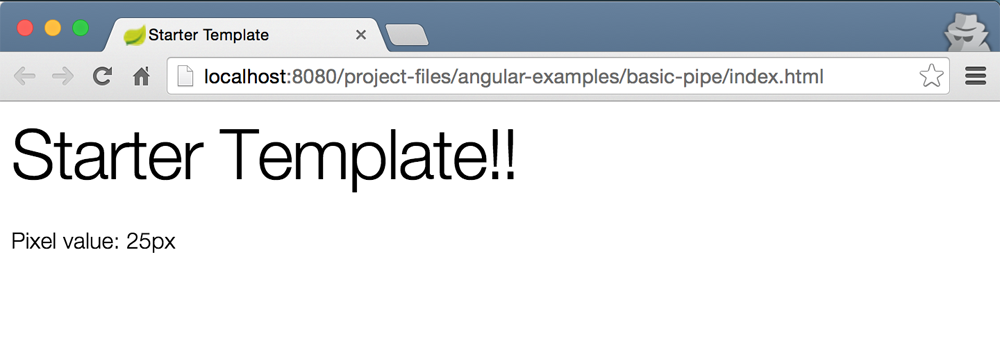
\includegraphics{images/basic-pipe.png}
\caption{Running the pixelPipe in the browser}
\end{figure}

\subsubsection{Chaining Pipes}\label{chaining-pipes}

Let's continue where we left off with the ``pixelPipe'' and add another
pipe called ``round'' that rounds down given values, that is:

\begin{verbatim}
25.3 | round | pixel -> 25px
\end{verbatim}

The project files for this section are in
\href{https://github.com/aminmeyghani/angular2-intro/tree/master/project-files/angular-examples/pipes/pipe-chaining}{angular2-intro/project-files/angular-examples/pipes/pipe-chaining}.

We are going to add the ``roundPipe'' to our ``basic-pipe'' project.
Let's get started by adding the \texttt{round.pipe.ts} file in the root
of the project:

\begin{Shaded}
\begin{Highlighting}[numbers=left,,]
\KeywordTok{import \{Pipe\} from 'angular2/core';}
\FunctionTok{@Pipe}\NormalTok{(\{name: 'round'\})}
\NormalTok{export }\KeywordTok{class} \NormalTok{RoundPipe \{}
  \FunctionTok{transform} \NormalTok{(input) \{}
    \KeywordTok{return} \NormalTok{Math.}\FunctionTok{floor}\NormalTok{(+input); }\CommentTok{// <- convert input to number and then floor it.}
  \NormalTok{\}}
\NormalTok{\}}
\end{Highlighting}
\end{Shaded}

This Pipe is not complicated at all. We are just returning the floor of
the input. We are also converting the input to number by putting a
\texttt{+} before input.

Now, let's import the pipe into our \texttt{main.ts} file:

\begin{Shaded}
\begin{Highlighting}[numbers=left,,]
\KeywordTok{import \{Component\} from 'angular2/core';}
\KeywordTok{import \{bootstrap\} from 'angular2/platform/browser';}
\KeywordTok{import \{PixelPipe\} from './pixel.pipe';}
\KeywordTok{import \{RoundPipe\} from './round.pipe';} \CommentTok{// <- importing `RoundPipe`}
\end{Highlighting}
\end{Shaded}

and then we have to add the pipe to the list of pipe array:

\begin{Shaded}
\begin{Highlighting}[numbers=left,,]
\FunctionTok{@Component}\NormalTok{(\{}
  \NormalTok{selector: 'app',}
  \NormalTok{templateUrl : 'templates/app.}\FunctionTok{tpl}\NormalTok{.}\FunctionTok{html}\NormalTok{',}
  \NormalTok{pipes: [PixelPipe, RoundPipe] }\CommentTok{// <- registering the pipe}
\NormalTok{\})}
\end{Highlighting}
\end{Shaded}

after that we are going to add the following to our
\texttt{templates/app.tpl.html} file:

\begin{Shaded}
\begin{Highlighting}[numbers=left,,]
\KeywordTok{<p>}\NormalTok{Pixel value: \{\{ 34.4 | round | pixel \}\}}\KeywordTok{</p>}
\end{Highlighting}
\end{Shaded}

After running the app you should see \texttt{34.px} as the output on the
page.

\subsubsection{Pipes with Parameters}\label{pipes-with-parameters}

In this section we are going to extend our `pixel' pipe to accept an
optional parameter to set the unit. As a result, we are going to rename
the `pixel' pipe to `unit' to make it more generic. This pipe will take
the unit as an optional argument. If no argument is passed, it will
default to `px'. That is:

\begin{verbatim}
25 | unit -> 25px
25 | unit:'em' -> 25em
34.5 | round | unit:'%' -> 34%
\end{verbatim}

You can look at the project files in
\href{https://github.com/aminmeyghani/angular2-intro/tree/master/project-files/angular-examples/pipes/pipe-unit}{angular2-intro/project-files/angular-examples/pipes/pipe-unit}..
AFter refactoring the name of the Pipe, we just need to change the
implementation of the ``UnitPipe'':

\textbf{\texttt{unit.pipe.ts}}

\begin{Shaded}
\begin{Highlighting}[numbers=left,,]
\KeywordTok{import \{Pipe\} from 'angular2/core';}
\FunctionTok{@Pipe}\NormalTok{(\{name: 'unit'\})}
\NormalTok{export }\KeywordTok{class} \NormalTok{UnitPipe \{}
  \FunctionTok{transform}\NormalTok{(input, args:string) \{}
    \DataTypeTok{const} \NormalTok{unit = args[}\DecValTok{0}\NormalTok{] || 'px';}
    \KeywordTok{return} \NormalTok{input + unit;}
  \NormalTok{\}}
\NormalTok{\}}
\end{Highlighting}
\end{Shaded}

\begin{itemize}
\tightlist
\item
  On line 5, we are grabbing the first parameter that is passed in and
  setting it to the \texttt{unit} variable. And if the value is not set,
  we are setting `px' as the default value.
\item
  And finally we are returning \texttt{input\ +\ unit}.
\end{itemize}

That's basically all we have to do. Note that you can pass multiple
parameters separated by \texttt{:} and they all become available in the
\texttt{args} array. So if you wanted to expand this pipe, this is how
your template would look like:

\begin{Shaded}
\begin{Highlighting}[numbers=left,,]
\NormalTok{\{\{ 25 | unit:'em':2\}\}}
\end{Highlighting}
\end{Shaded}

And the \texttt{args} array would be:
\texttt{{[}\textquotesingle{}em\textquotesingle{},\ 2{]}}.

\subsubsection{Async Pipes}\label{async-pipes}

Async Pipes can be used for values that will be resolved after some
asynchronous operation like getting a value after making a http call.

\textbf{TODO}

\subsubsection{Built-in Pipes}\label{built-in-pipes}

In this section we are going to look at the pipes that Angular provides
out of the box.

\begin{itemize}
\tightlist
\item
  \href{https://angular.io/docs/ts/latest/api/common/AsyncPipe-class.html}{AsyncPipe}:
  used to work with asynchronous values
\item
  \href{https://angular.io/docs/ts/latest/api/common/CurrencyPipe-class.html}{CurrencyPipe}:
  used to format a number as a local currency
\item
  \href{https://angular.io/docs/ts/latest/api/common/DatePipe-class.html}{DatePipe}:
  used to format a date object to a readable string
\item
  \href{https://angular.io/docs/ts/latest/api/common/DecimalPipe-class.html}{DecimalPipe}:
  used to format numbers
\item
  \href{https://angular.io/docs/ts/latest/api/common/JsonPipe-class.html}{JsonPipe}:
  calls \texttt{JSON.stringify} on the input and useful for debugging
\item
  \href{https://angular.io/docs/ts/latest/api/common/LowerCasePipe-class.html}{LowerCasePipe}:
  used to convert a string to lowercase letters
\item
  \href{https://angular.io/docs/ts/latest/api/common/PercentPipe-class.html}{PercentPipe}:
  used to format a number as percentage
\item
  \href{https://angular.io/docs/ts/latest/api/common/SlicePipe-class.html}{SlicePipe}:
  used to create a subset of list or string
\item
  \href{https://angular.io/docs/ts/latest/api/common/UpperCasePipe-class.html}{UpperCasePipe}:
  used to transform a text to upper case
\end{itemize}

\paragraph{Date}\label{date}

\begin{Shaded}
\begin{Highlighting}[numbers=left,,]
\NormalTok{\{\{ input | date:optionalFormat\}\}}
\end{Highlighting}
\end{Shaded}

\begin{itemize}
\tightlist
\item
  \texttt{input}: a date object or a number (milliseconds since UTC
  epoch)
\item
  \texttt{optionalFormat}: a string used to format the output. It
  specifies which components of date and time to include in the output
\end{itemize}

\textbf{Using predefined formats}

Usage Example:
\texttt{\{\{\ input\ \textbar{}\ date:\textquotesingle{}short\textquotesingle{}\}\}}

\begin{longtable}[c]{@{}ll@{}}
\toprule
\begin{minipage}[b]{0.20\columnwidth}\raggedright\strut
Name
\strut\end{minipage} &
\begin{minipage}[b]{0.37\columnwidth}\raggedright\strut
Example
\strut\end{minipage}\tabularnewline
\midrule
\endhead
\begin{minipage}[t]{0.20\columnwidth}\raggedright\strut
\texttt{short}
\strut\end{minipage} &
\begin{minipage}[t]{0.37\columnwidth}\raggedright\strut
9/3/2010, 12:05 PM
\strut\end{minipage}\tabularnewline
\begin{minipage}[t]{0.20\columnwidth}\raggedright\strut
\texttt{shortDate}
\strut\end{minipage} &
\begin{minipage}[t]{0.37\columnwidth}\raggedright\strut
9/3/2010
\strut\end{minipage}\tabularnewline
\begin{minipage}[t]{0.20\columnwidth}\raggedright\strut
\texttt{medium}
\strut\end{minipage} &
\begin{minipage}[t]{0.37\columnwidth}\raggedright\strut
Sep 3, 2010, 12:05:08 PM
\strut\end{minipage}\tabularnewline
\begin{minipage}[t]{0.20\columnwidth}\raggedright\strut
\texttt{mediumDate}
\strut\end{minipage} &
\begin{minipage}[t]{0.37\columnwidth}\raggedright\strut
Sep 3, 2010
\strut\end{minipage}\tabularnewline
\begin{minipage}[t]{0.20\columnwidth}\raggedright\strut
\texttt{longDate}
\strut\end{minipage} &
\begin{minipage}[t]{0.37\columnwidth}\raggedright\strut
September 3, 2010
\strut\end{minipage}\tabularnewline
\begin{minipage}[t]{0.20\columnwidth}\raggedright\strut
\texttt{fullDate}
\strut\end{minipage} &
\begin{minipage}[t]{0.37\columnwidth}\raggedright\strut
Friday, September 3, 2010
\strut\end{minipage}\tabularnewline
\begin{minipage}[t]{0.20\columnwidth}\raggedright\strut
\texttt{shortTime}
\strut\end{minipage} &
\begin{minipage}[t]{0.37\columnwidth}\raggedright\strut
12:05 PM
\strut\end{minipage}\tabularnewline
\begin{minipage}[t]{0.20\columnwidth}\raggedright\strut
\texttt{mediumTime}
\strut\end{minipage} &
\begin{minipage}[t]{0.37\columnwidth}\raggedright\strut
12:05:08 PM
\strut\end{minipage}\tabularnewline
\bottomrule
\end{longtable}

\textbf{Using Custom Formats}

\begin{itemize}
\tightlist
\item
  Generally speaking every date object has a year, month, day, hour,
  minute, and second.
\item
  Using a custom string, you can specify which component you would like
  to include in the output.
\end{itemize}

\begin{longtable}[c]{@{}lllllll@{}}
\toprule
\begin{minipage}[b]{0.07\columnwidth}\raggedright\strut
Year
\strut\end{minipage} &
\begin{minipage}[b]{0.19\columnwidth}\raggedright\strut
Month
\strut\end{minipage} &
\begin{minipage}[b]{0.06\columnwidth}\raggedright\strut
Day
\strut\end{minipage} &
\begin{minipage}[b]{0.15\columnwidth}\raggedright\strut
Weekday
\strut\end{minipage} &
\begin{minipage}[b]{0.14\columnwidth}\raggedright\strut
Hour
\strut\end{minipage} &
\begin{minipage}[b]{0.10\columnwidth}\raggedright\strut
Minute
\strut\end{minipage} &
\begin{minipage}[b]{0.10\columnwidth}\raggedright\strut
Second
\strut\end{minipage}\tabularnewline
\midrule
\endhead
\begin{minipage}[t]{0.07\columnwidth}\raggedright\strut
y
\strut\end{minipage} &
\begin{minipage}[t]{0.19\columnwidth}\raggedright\strut
M, MMM, MMMM
\strut\end{minipage} &
\begin{minipage}[t]{0.06\columnwidth}\raggedright\strut
d
\strut\end{minipage} &
\begin{minipage}[t]{0.15\columnwidth}\raggedright\strut
EEE, EEEE
\strut\end{minipage} &
\begin{minipage}[t]{0.14\columnwidth}\raggedright\strut
j, h, H
\strut\end{minipage} &
\begin{minipage}[t]{0.10\columnwidth}\raggedright\strut
m
\strut\end{minipage} &
\begin{minipage}[t]{0.10\columnwidth}\raggedright\strut
s
\strut\end{minipage}\tabularnewline
\begin{minipage}[t]{0.07\columnwidth}\raggedright\strut
2016
\strut\end{minipage} &
\begin{minipage}[t]{0.19\columnwidth}\raggedright\strut
1, Jan, January
\strut\end{minipage} &
\begin{minipage}[t]{0.06\columnwidth}\raggedright\strut
1
\strut\end{minipage} &
\begin{minipage}[t]{0.15\columnwidth}\raggedright\strut
Sun, Sunday
\strut\end{minipage} &
\begin{minipage}[t]{0.14\columnwidth}\raggedright\strut
1, 1 AM, 1
\strut\end{minipage} &
\begin{minipage}[t]{0.10\columnwidth}\raggedright\strut
1
\strut\end{minipage} &
\begin{minipage}[t]{0.10\columnwidth}\raggedright\strut
1
\strut\end{minipage}\tabularnewline
\bottomrule
\end{longtable}

Note that every single letter identifier can be used twice to denote a
double digit numeric value. For example, \texttt{yy} will result in
\texttt{15} for the year value. Below is a table just to be thorough:

\textbf{Double Digit}

\begin{longtable}[c]{@{}llllll@{}}
\toprule
\begin{minipage}[b]{0.08\columnwidth}\raggedright\strut
Year
\strut\end{minipage} &
\begin{minipage}[b]{0.09\columnwidth}\raggedright\strut
Month
\strut\end{minipage} &
\begin{minipage}[b]{0.07\columnwidth}\raggedright\strut
Day
\strut\end{minipage} &
\begin{minipage}[b]{0.20\columnwidth}\raggedright\strut
Hour
\strut\end{minipage} &
\begin{minipage}[b]{0.10\columnwidth}\raggedright\strut
Minute
\strut\end{minipage} &
\begin{minipage}[b]{0.10\columnwidth}\raggedright\strut
Second
\strut\end{minipage}\tabularnewline
\midrule
\endhead
\begin{minipage}[t]{0.08\columnwidth}\raggedright\strut
yy
\strut\end{minipage} &
\begin{minipage}[t]{0.09\columnwidth}\raggedright\strut
MM
\strut\end{minipage} &
\begin{minipage}[t]{0.07\columnwidth}\raggedright\strut
dd
\strut\end{minipage} &
\begin{minipage}[t]{0.20\columnwidth}\raggedright\strut
jj, hh, HH
\strut\end{minipage} &
\begin{minipage}[t]{0.10\columnwidth}\raggedright\strut
mm
\strut\end{minipage} &
\begin{minipage}[t]{0.10\columnwidth}\raggedright\strut
ss
\strut\end{minipage}\tabularnewline
\begin{minipage}[t]{0.08\columnwidth}\raggedright\strut
16
\strut\end{minipage} &
\begin{minipage}[t]{0.09\columnwidth}\raggedright\strut
01
\strut\end{minipage} &
\begin{minipage}[t]{0.07\columnwidth}\raggedright\strut
01
\strut\end{minipage} &
\begin{minipage}[t]{0.20\columnwidth}\raggedright\strut
01, 01 AM, 01
\strut\end{minipage} &
\begin{minipage}[t]{0.10\columnwidth}\raggedright\strut
01
\strut\end{minipage} &
\begin{minipage}[t]{0.10\columnwidth}\raggedright\strut
01
\strut\end{minipage}\tabularnewline
\bottomrule
\end{longtable}

Details for Month/Weekday/Hour are summarized in the tables below:

\textbf{Month Details}

\begin{longtable}[c]{@{}lll@{}}
\toprule
\begin{minipage}[b]{0.10\columnwidth}\raggedright\strut
M
\strut\end{minipage} &
\begin{minipage}[b]{0.15\columnwidth}\raggedright\strut
MMM
\strut\end{minipage} &
\begin{minipage}[b]{0.15\columnwidth}\raggedright\strut
MMMM
\strut\end{minipage}\tabularnewline
\midrule
\endhead
\begin{minipage}[t]{0.10\columnwidth}\raggedright\strut
Digit
\strut\end{minipage} &
\begin{minipage}[t]{0.15\columnwidth}\raggedright\strut
Abbr Name
\strut\end{minipage} &
\begin{minipage}[t]{0.15\columnwidth}\raggedright\strut
Full Name
\strut\end{minipage}\tabularnewline
\begin{minipage}[t]{0.10\columnwidth}\raggedright\strut
1
\strut\end{minipage} &
\begin{minipage}[t]{0.15\columnwidth}\raggedright\strut
Jan
\strut\end{minipage} &
\begin{minipage}[t]{0.15\columnwidth}\raggedright\strut
January
\strut\end{minipage}\tabularnewline
\bottomrule
\end{longtable}

\textbf{Weekday Details}

\begin{longtable}[c]{@{}ll@{}}
\toprule
\begin{minipage}[b]{0.16\columnwidth}\raggedright\strut
EEE
\strut\end{minipage} &
\begin{minipage}[b]{0.16\columnwidth}\raggedright\strut
EEEE
\strut\end{minipage}\tabularnewline
\midrule
\endhead
\begin{minipage}[t]{0.16\columnwidth}\raggedright\strut
Abbr Name
\strut\end{minipage} &
\begin{minipage}[t]{0.16\columnwidth}\raggedright\strut
Full Name
\strut\end{minipage}\tabularnewline
\begin{minipage}[t]{0.16\columnwidth}\raggedright\strut
Sun
\strut\end{minipage} &
\begin{minipage}[t]{0.16\columnwidth}\raggedright\strut
Sunday
\strut\end{minipage}\tabularnewline
\bottomrule
\end{longtable}

\textbf{Hour Details}

\begin{longtable}[c]{@{}lll@{}}
\toprule
\begin{minipage}[b]{0.10\columnwidth}\raggedright\strut
j
\strut\end{minipage} &
\begin{minipage}[b]{0.19\columnwidth}\raggedright\strut
h
\strut\end{minipage} &
\begin{minipage}[b]{0.14\columnwidth}\raggedright\strut
H
\strut\end{minipage}\tabularnewline
\midrule
\endhead
\begin{minipage}[t]{0.10\columnwidth}\raggedright\strut
Digit
\strut\end{minipage} &
\begin{minipage}[t]{0.19\columnwidth}\raggedright\strut
Hour12 AM/PM
\strut\end{minipage} &
\begin{minipage}[t]{0.14\columnwidth}\raggedright\strut
Military
\strut\end{minipage}\tabularnewline
\begin{minipage}[t]{0.10\columnwidth}\raggedright\strut
13
\strut\end{minipage} &
\begin{minipage}[t]{0.19\columnwidth}\raggedright\strut
1 PM
\strut\end{minipage} &
\begin{minipage}[t]{0.14\columnwidth}\raggedright\strut
13
\strut\end{minipage}\tabularnewline
\bottomrule
\end{longtable}

\paragraph{Slice}\label{slice}

\begin{itemize}
\tightlist
\item
  The slice pipe is useful when you want a subset of a list or string.
  One of the common use cases are in when iterating over a list with
  \texttt{ngFor} for example.
\end{itemize}

\textbf{TODO}

\paragraph{Decimal}\label{decimal}

\begin{itemize}
\tightlist
\item
  Used for formatting numbers given a decimal formatter
\end{itemize}

\textbf{TODO}

\paragraph{Percent}\label{percent}

\textbf{TODO}

\paragraph{Currency}\label{currency}

\textbf{TODO}

\paragraph{Async}\label{async}

\textbf{TODO}

\paragraph{Json}\label{json}

\textbf{TODO}

\paragraph{LowerCase}\label{lowercase}

\textbf{TODO}

\paragraph{UpperCase}\label{uppercase}

\textbf{TODO}

\subsection{Dependency Injection}\label{dependency-injection}

Dependency Injection is a coding pattern in which a class receives its
dependencies from external sources rather than creating them itself. In
order to achieve Dependency Injection we need a Dependency
InjectionFramework to handle the dependencies for us. Using a DI
framework, you simply ask for a class from the injector instead of
worrying about the dependencies inside the class itself.

Angular has a standalone module that handles Dependency Injection. This
framework can also be used in non-Angular applications to handle
Dependency Injection.

\textbf{TODO}

\subsection{Services and Providers}\label{services-and-providers}

\begin{itemize}
\item
  A service is nothing more than a class in Angular 2. It remains
  nothing more than a class until we register it with the Angular
  injector.
\item
  When you bootstrap your app, Angular creates an injector on the fly
  that can inject services and other dependencies throughout the app.
\item
  You can register the service or the dependencies during when
  bootstrapping the app or when defining a component.
\item
  If you have a class called \texttt{MyService}, you can register it
  with the Injector and then you can inject it everywhere:

\begin{Shaded}
\begin{Highlighting}[numbers=left,,]
\FunctionTok{bootstrap}\NormalTok{(App, [MyService]); }\CommentTok{// second param is an array of providers}
\end{Highlighting}
\end{Shaded}
\item
  Providers is a way to specify what services are available inside the
  component in a hierarchical fashion.
\item
  A provider can be a class, a value or a factory.
\item
  Providers create the instances of the things that we ask the injector
  to inject.
\item
  \texttt{{[}SomeService{]};} is short for
  \texttt{{[}provide(SomeService,\ \{useClass:SomeService\}){]};} where
  the first param is the token, and the second is the definition object.
\item
  A simple object can be passed to the Injector to create a Value
  Provider:

\begin{Shaded}
\begin{Highlighting}[numbers=left,,]
\FunctionTok{beforeEachProviders}\NormalTok{(() => \{}
  \NormalTok{let someService = \{ getData: () => [] \};}
  \CommentTok{// using `useValue` instead of `useClass`}
  \KeywordTok{return} \NormalTok{[ }\FunctionTok{provide}\NormalTok{(SomeSvc, \{useValue: someService\}) ];}
\NormalTok{\});}
\end{Highlighting}
\end{Shaded}
\item
  You can also use a factory as a provider.
\item
  You can use a factory function that creates a properly configured
  Service:

\begin{Shaded}
\begin{Highlighting}[numbers=left,,]
\NormalTok{let myServiceFactory = (dx: DepX, dy: DepY) => \{}
  \KeywordTok{return} \KeywordTok{new} \FunctionTok{MyService}\NormalTok{(dx, dy.}\FunctionTok{value}\NormalTok{);}
\NormalTok{\}}

\CommentTok{// provider definition object.}
\NormalTok{let myServiceDefinition = \{}
   \NormalTok{useFactory: myServiceFactory,}
   \NormalTok{deps: [DepX, DepY]}
\NormalTok{\};}

\CommentTok{// create provider and bootstrap}
\NormalTok{let myServiceProvider = }\FunctionTok{provide}\NormalTok{(MyService, myServiceDefinition);}
\FunctionTok{bootstrap}\NormalTok{(AppComponent, [myServiceProvider, DepX, DepY]);}
\end{Highlighting}
\end{Shaded}
\item
  Defining object dependencies is simple. You can make a plain
  JavaScript object available for injection using a string-based token
  and the \texttt{@Inject} decorator:

\begin{Shaded}
\begin{Highlighting}[numbers=left,,]
\NormalTok{var myObj = \{\};}

\FunctionTok{bootstrap}\NormalTok{(AppComponent, [}
  \FunctionTok{provide}\NormalTok{('coolObjToken', \{useValue: myObj\})}
\NormalTok{]);}

\CommentTok{// and you can inject it to a component}

\KeywordTok{import} \NormalTok{\{Inject\} from 'angular2/core'}
\FunctionTok{constructor}\NormalTok{(dx: DepX, }\FunctionTok{@Inject}\NormalTok{('coolObjToken') config)}
\end{Highlighting}
\end{Shaded}
\end{itemize}

\subsubsection{Simple Service}\label{simple-service}

In this section we are going to make a simple service and use it in our
root component.

\textbf{Project Files}

The project files for this section are in
\href{https://github.com/aminmeyghani/angular2-intro/tree/master/project-files/angular-examples/services/simple-service}{angular2-intro/project-files/angular-examples/services/simple-service};

\textbf{Getting Started}

Let's get started by creating a class, called \texttt{StudentSvc} that
represents our service:

\begin{Shaded}
\begin{Highlighting}[numbers=left,,]
\KeywordTok{class} \NormalTok{StudentSvc \{}
  \KeywordTok{private} \NormalTok{students: any[];}
  \FunctionTok{constructor}\NormalTok{() \{}
    \KeywordTok{this}\NormalTok{.}\FunctionTok{students} \NormalTok{= [}
      \NormalTok{\{name: 'Tom', id: }\DecValTok{1}\NormalTok{\},}
      \NormalTok{\{name: 'John', id: }\DecValTok{2}\NormalTok{\},}
      \NormalTok{\{name: 'Kim', id: }\DecValTok{3}\NormalTok{\},}
      \NormalTok{\{name: 'Liz', id: }\DecValTok{4}\NormalTok{\}}
    \NormalTok{];}
  \NormalTok{\}}
  \FunctionTok{getAll}\NormalTok{() \{}
    \KeywordTok{return} \KeywordTok{this}\NormalTok{.}\FunctionTok{students}\NormalTok{;}
  \NormalTok{\}}
\NormalTok{\}}
\end{Highlighting}
\end{Shaded}

There is nothing special about this class. It's just a class the has a
method to return the list of all students. Now, we are going to make it
special by decorating it with the \texttt{Injectable} decorator. But,
first we need to import \texttt{Injectable} from Angular:

\begin{Shaded}
\begin{Highlighting}[numbers=left,,]
\KeywordTok{import \{Injectable\} from 'angular2/core';}
\end{Highlighting}
\end{Shaded}

After importing the \texttt{Injectable} metadata class, we can decorate
our class:

\begin{Shaded}
\begin{Highlighting}[numbers=left,,]
\CommentTok{/**}
\CommentTok{ * Student service}
\CommentTok{ */}
\FunctionTok{@Injectable}\NormalTok{() }\CommentTok{// <- decorating with `Injectable`}
\KeywordTok{class} \NormalTok{StudentSvc \{}
  \KeywordTok{private} \NormalTok{students: any[];}
  \FunctionTok{constructor}\NormalTok{() \{}
   \CommentTok{// ...}
  \NormalTok{\}}
  \CommentTok{// ...}
\NormalTok{\}}
\end{Highlighting}
\end{Shaded}

Now we have an injectable class and the injector would know how to
create an instance of it when we need to inject it. And that's what we
are going to do next. We are going to add \texttt{StudentSvc} in the
list of \texttt{viewProviders} of the root component:

\begin{Shaded}
\begin{Highlighting}[numbers=left,,]
\FunctionTok{@Component}\NormalTok{(\{}
  \NormalTok{selector: 'app',}
  \NormalTok{templateUrl : 'templates/app.}\FunctionTok{tpl}\NormalTok{.}\FunctionTok{html}\NormalTok{',}
  \NormalTok{viewProviders: [StudentSvc] }\CommentTok{// <- registering the service}
\NormalTok{\})}
\end{Highlighting}
\end{Shaded}

The last thing we need to do is to inject the service in the constructor
of our root component:

\begin{Shaded}
\begin{Highlighting}[numbers=left,,]
\KeywordTok{class} \NormalTok{Root  \{}
  \KeywordTok{private} \NormalTok{name: string;}
  \KeywordTok{private} \NormalTok{students: any[];}
  \FunctionTok{constructor} \NormalTok{(studentSvc: StudentSvc) \{ }\CommentTok{// <- injecting the service}
    \KeywordTok{this}\NormalTok{.}\FunctionTok{name} \NormalTok{= 'Simple Service Demo';}
    \KeywordTok{this}\NormalTok{.}\FunctionTok{students} \NormalTok{= studentSvc.}\FunctionTok{getAll}\NormalTok{(); }\CommentTok{// <- calling the `getAll` method}
  \NormalTok{\}}
\NormalTok{\}}
\end{Highlighting}
\end{Shaded}

\begin{itemize}
\item
  In the constructor, we are defining a variable to be of type
  \texttt{StudentSvc}. By doing that the injector will create an
  instance from the \texttt{StudentSvc} to be used
\item
  And on line 6 we are calling the \texttt{getAll} method from the
  service to get a list of all students.
\end{itemize}

Finally, we can verify that the \texttt{getAll} method is actually
called by printing the students in the template:

\textbf{\texttt{app.tpl.html}}

\begin{Shaded}
\begin{Highlighting}[numbers=left,,]
\KeywordTok{<h1>}\NormalTok{\{\{ name \}\}}\KeywordTok{</h1>}

\KeywordTok{<ul>}
  \KeywordTok{<li} \ErrorTok{*ngFor}\OtherTok{=}\StringTok{"#student of students"}\KeywordTok{>}\NormalTok{Name: \{\{ student.name \}\}, id: \{\{ student.id \}\}}\KeywordTok{</li>}
\KeywordTok{</ul>}
\end{Highlighting}
\end{Shaded}

and it would output:

\begin{verbatim}
Name: Tom, id: 1
Name: John, id: 2
Name: Kim, id: 3
Name: Liz, id: 4
\end{verbatim}

\subsection{Data and State Management}\label{data-and-state-management}

\begin{itemize}
\tightlist
\item
  Angular is flexible and doesn't prescribe a recipe for managing data
  in your apps
\item
  Since observables are integrated into Angular, you can take advantage
  of observables to manage data and state
\item
  You ca use services to manage streams that emit models
\item
  Components can subscribe to the streams maintained by services and
  render accordingly.

  \begin{itemize}
  \tightlist
  \item
    For example, you can have a service for a Todo app that contains a
    stream of todos and a \texttt{ListComponent} can listen for todos
    and render when a new task is added.
  \item
    You may have another component that listens for the user that has
    been assigned to a task provided by a service.
  \end{itemize}
\item
  The steps for creating different parts of an app can be summarized in
  three steps:

  \begin{itemize}
  \tightlist
  \item
    Defining a Model using a class
  \item
    Defining the service
  \item
    Defining the component
  \end{itemize}
\end{itemize}

\subsubsection{Observables}\label{observables}

\begin{itemize}
\item
  Observables can help manage async data
\item
  Observables are similar to Promises but with a lot of differences
\item
  Observables emit multiple values over time as opposed to one
\item
  Angular embraces observables using the RxJS library.
\item
  Observables emit events and observers observe observables.
\item
  An observer \emph{subscribes} to events emitted from an observable.
\item
  RxJS has an object called \emph{subject} that can be used both as an
  observer or an observable. \emph{Subject} can be imported from
  \texttt{RxJS} very easily:

\begin{Shaded}
\begin{Highlighting}[numbers=left,,]
\KeywordTok{import \{Subject\} from 'rxjs/Subject';}
\end{Highlighting}
\end{Shaded}
\item
  A subscription can be canceled by calling the \texttt{unsubscribe}
  method.
\end{itemize}

\textbf{TODO}

\subsubsection{State Management with
Observables}\label{state-management-with-observables}

\begin{itemize}
\tightlist
\item
  There are several ways to manage state, one of them is using
  observables
\item
  Observables can be used to represent the state of the app
\item
  Changes in the state are represented as an observable
\end{itemize}

\textbf{TODO}

\subsection{Http}\label{http}

\begin{itemize}
\tightlist
\item
  Using the \texttt{Http} class, you can interact with API endpoints
\item
  Http is available as an injectable class
\item
  \texttt{Http} has a request method that returns an Observable which
  will emit a single Response when a response is received.
\item
  You can inject \texttt{http} in the constructor of a class:
  \texttt{constructor(http:\ Http)\ \{...\}}
\end{itemize}

\subsubsection{Getting Data from Server}\label{getting-data-from-server}

In this section we are going to use the \texttt{http} class to get a
list of students from a server by hitting \texttt{/api/students}

\textbf{Project Files}

The project files for this section are in
\href{https://github.com/aminmeyghani/angular2-intro/tree/master/project-files/angular-examples/http/get-students}{angular2-intro/project-files/angular-examples/http/get-students}

\textbf{Getting Started}

Before anything, let's add the \texttt{http.js} file from Angular's
bundle. In your \texttt{index.html} file add the following to the head
tag:

\begin{Shaded}
\begin{Highlighting}[numbers=left,,]
\KeywordTok{<script}\OtherTok{ src=}\StringTok{"/node_modules/angular2/bundles/http.js"}\KeywordTok{></script>}
\end{Highlighting}
\end{Shaded}

After that, we are going to make a service that handles getting data
from the endpoint. We are going to call this \texttt{StudentSvc}:

\begin{Shaded}
\begin{Highlighting}[numbers=left,,]
\FunctionTok{@Injectable}\NormalTok{()}
\KeywordTok{class} \NormalTok{StudentSvc \{}
  \FunctionTok{constructor}\NormalTok{(}\KeywordTok{private} \NormalTok{http: Http) \{\} }\CommentTok{/* Inject Http */}
  \FunctionTok{getStudents}\NormalTok{(): Observable<Response> \{}
    \KeywordTok{return} \KeywordTok{this}\NormalTok{.}\FunctionTok{http}\NormalTok{.}\FunctionTok{get}\NormalTok{('/api/students');}
  \NormalTok{\}}
\NormalTok{\}}
\end{Highlighting}
\end{Shaded}

\begin{itemize}
\tightlist
\item
  On line 1, we are using the \texttt{Injectable} decorator to make our
  class injectable
\item
  In the constructor we are injecting the \texttt{Http} service and
  making a reference to it in a private variable \texttt{http}
\item
  The \texttt{getStudents} method makes a \texttt{GET} call to our local
  endpoint an returns an \texttt{Observable}
\end{itemize}

Now that we have the \texttt{StudentSvc} service, we can create a
component and inject the \texttt{StudentSvc} to it:

\begin{Shaded}
\begin{Highlighting}[numbers=left,,]
\FunctionTok{@Component}\NormalTok{(\{}
  \NormalTok{selector: 'app',}
  \NormalTok{templateUrl :'templates/app.}\FunctionTok{tpl}\NormalTok{.}\FunctionTok{html}\NormalTok{',}
  \NormalTok{providers: [StudentSvc] }\CommentTok{// <- adding to the list of providers}
\NormalTok{\})}
\end{Highlighting}
\end{Shaded}

In addition to the \texttt{StudentSvc}, we also need to add
\texttt{HTTP\_PROVIDERS} in the providers array:

\begin{Shaded}
\begin{Highlighting}[numbers=left,,]
\FunctionTok{@Component}\NormalTok{(\{}
  \NormalTok{selector: 'app',}
  \NormalTok{templateUrl :'templates/app.}\FunctionTok{tpl}\NormalTok{.}\FunctionTok{html}\NormalTok{',}
  \NormalTok{providers: [HTTP_PROVIDERS, StudentSvc] }\CommentTok{// <- adding `HTTP_PROVIDERS`}
\NormalTok{\})}
\end{Highlighting}
\end{Shaded}

After adding the providers, we can define the component class:

\begin{Shaded}
\begin{Highlighting}[numbers=left,,]
\FunctionTok{@Component}\NormalTok{(\{...\})}
\KeywordTok{class} \NormalTok{HttpGetExample  \{}
  \KeywordTok{private} \NormalTok{name: string;}
  \KeywordTok{private} \NormalTok{students: Observable<Response>;}
  \FunctionTok{constructor} \NormalTok{(studentSvc: StudentSvc) \{}
    \KeywordTok{this}\NormalTok{.}\FunctionTok{name} \NormalTok{= 'HTTP Get';}
    \NormalTok{studentSvc.}\FunctionTok{getStudents}\NormalTok{().}\FunctionTok{subscribe}\NormalTok{(resp => }\KeywordTok{this}\NormalTok{.}\FunctionTok{students} \NormalTok{= resp.}\FunctionTok{json}\NormalTok{());}
  \NormalTok{\}}
\NormalTok{\}}
\end{Highlighting}
\end{Shaded}

If you notice, we are injecting the \texttt{StudentSvc} in the
constructor and we are calling the \texttt{getStudents} method in the
constructor. The \texttt{getStudents} returns an observable that we can
subscribe to get the data out as they arrive. We also call the
\texttt{json} method on each response to get the JSON data.

After getting the data, we can print the result in the view:

\textbf{\texttt{app.tpl.html}}

\begin{Shaded}
\begin{Highlighting}[numbers=left,,]
\KeywordTok{<h1>}\NormalTok{\{\{ name \}\}}\KeywordTok{</h1>}
\KeywordTok{<ul>}
  \KeywordTok{<li} \ErrorTok{*ngFor}\OtherTok{=}\StringTok{"#student of students"}\KeywordTok{>}
    \NormalTok{\{\{ student.name \}\}, \{\{ student.lastname \}\}}
  \KeywordTok{</li>}
\KeywordTok{</ul>}
\end{Highlighting}
\end{Shaded}

Here we are using the built-in \texttt{ngFor} directive to loop through
the array of students and print their name and last name to the page.

\subsection{Working with Forms}\label{working-with-forms}

Angular has convenient methods for working with forms, including
validation.

\textbf{TODO}

\subsection{Angular Router}\label{angular-router}

Angular has a stand-alone module responsible for handling routing.

\textbf{TODO}

\subsection{Unit Testing}\label{unit-testing}

Unit testing with Angular requires some set up. First, let's gather all
the libraries and modules that we need.

\textbf{TODO}

\section{Deep Dive}\label{deep-dive}

Let's deep dive into Angular and RxJS concepts

\subsection{Components in Depth}\label{components-in-depth}

\begin{itemize}
\tightlist
\item
  A component declares a reusable building block of an app
\item
  A TypeScript class is used to define a component coupled with the
  \texttt{@component} decorator
\end{itemize}

The \texttt{@component} decorator defines the following:

\begin{itemize}
\item
  selector: \texttt{string} value defining the css selector targeting an
  html element
\item
  inputs: \texttt{array\ of\ string} values defining the inputs to the
  component
\item
  outputs: \texttt{array\ of\ string} values defining the output of the
  component
\item
  properties: \texttt{array\ of\ string} values defining the properties
\item
  events: \texttt{array\ of\ string} values defining the events
\item
  host?: \{{[}`string'{]}: `string'\},
\item
  providers: \texttt{array\ of\ objects}: defines the set of injectable
  objects that are visible to a directive/component and its light DOM
  children.
\item
  exportAs: \texttt{string} value defining the exported value
\item
  moduleId: \texttt{string} value defining the module id
\item
  viewProviders?: \texttt{array\ of\ objects}: defines the set of
  injectable objects that are visible to a directive/component view DOM
  children.
\item
  queries: \{{[}key: string{]}: any\},
\item
  changeDetection: \texttt{ChangeDetectionStrategy} object defining the
  strategy for detecting changes:

  \begin{itemize}
  \tightlist
  \item
    \texttt{ChangeDetectionStrategy.Default}: sets detector mode to
    \texttt{CheckAlways}
  \item
    \texttt{ChangeDetectionStrategy.OnPush}: sets detector mode to
    \texttt{CheckOnce}
  \item
    \texttt{ChangeDetectionStrategy.Detached}: change detector sub tree
    is not a part of the main tree and should be skipped
  \item
    \texttt{ChangeDetectionStrategy.CheckAlways}: after calling
    detectChanges the mode of the change detector will remain
    \texttt{CheckAlways}
  \item
    \texttt{ChangeDetectionStrategy.Checked}: change detector should be
    skipped until its mode changes to \texttt{CheckOnce}
  \item
    \texttt{ChangeDetectionStrategy.CheckOnce}: after calling
    detectChanges the mode of the change detector will become
    \texttt{Checked}
  \end{itemize}
\item
  templateUrl: \texttt{string} value for the url path to the template
\item
  template: \texttt{string} value for the template
\item
  styleUrls: \texttt{array\ of\ string} values defining url paths to css
  files
\item
  styles: \texttt{array\ of\ string} values defining css styles:

  \begin{itemize}
  \tightlist
  \item
    styles: {[}`.myclass \{ color: \#000;\}'{]},
  \end{itemize}
\item
  directives: \texttt{array} of directives used in the component
\item
  pipes: \texttt{array} of pipes used in the component
\item
  encapsulation: \texttt{ViewEncapsulation} value that defines template
  and style encapsulation options:

  \begin{itemize}
  \tightlist
  \item
    \texttt{ViewEncapsulation.None}: means do not provide any style
    encapsulation
  \item
    \texttt{ViewEncapsulation.Emulated}: No Shadow DOM but style
    encapsulation emulation using extra attributes on the DOM (default
    method)
  \item
    \texttt{ViewEncapsulation.Native}: means provide native shadow DOM
    encapsulation and styles appear in component's template inside the
    shadow root.
  \end{itemize}
\end{itemize}

\textbf{TODO}

\section{RxJS}\label{rxjs}

\begin{itemize}
\tightlist
\item
  RxJS is a library for reactive programming
\item
  Reactive programming is a natural way of thinking about asynchronous
  code which concerns itself with operations on event streams
\item
  RxJS is used in this paradigm to compose asynchronous data/event
  streams
\item
  Using the reactive paradigm, you can perform operations on streams
  using a consistent interface regardless of the data source
\item
  Streams of events/data are known as Observables, i.e.~a data/event
  stream = observable
\item
  A program can be just composed of different data streams (observables)
\end{itemize}

\textbf{TODO}

\begin{itemize}
\tightlist
\item
  \href{http://rxmarbles.com/}{Visualization}
\end{itemize}

\end{document}
